
\documentclass[10pt]{article} % For LaTeX2e
\usepackage{tmlr}
% If accepted, instead use the following line for the camera-ready submission:
% \usepackage[accepted]{tmlr}
% To de-anonymize and remove mentions to TMLR (for example for posting to preprint servers), instead use the following:
%\usepackage[preprint]{tmlr}

% Optional math commands from https://github.com/goodfeli/dlbook_notation.
%%%%% NEW MATH DEFINITIONS %%%%%

\usepackage{amsmath,amsfonts,bm}

% Mark sections of captions for referring to divisions of figures
\newcommand{\figleft}{{\em (Left)}}
\newcommand{\figcenter}{{\em (Center)}}
\newcommand{\figright}{{\em (Right)}}
\newcommand{\figtop}{{\em (Top)}}
\newcommand{\figbottom}{{\em (Bottom)}}
\newcommand{\captiona}{{\em (a)}}
\newcommand{\captionb}{{\em (b)}}
\newcommand{\captionc}{{\em (c)}}
\newcommand{\captiond}{{\em (d)}}

% Highlight a newly defined term
\newcommand{\newterm}[1]{{\bf #1}}


% Figure reference, lower-case.
\def\figref#1{figure~\ref{#1}}
% Figure reference, capital. For start of sentence
\def\Figref#1{Figure~\ref{#1}}
\def\twofigref#1#2{figures \ref{#1} and \ref{#2}}
\def\quadfigref#1#2#3#4{figures \ref{#1}, \ref{#2}, \ref{#3} and \ref{#4}}
% Section reference, lower-case.
\def\secref#1{section~\ref{#1}}
% Section reference, capital.
\def\Secref#1{Section~\ref{#1}}
% Reference to two sections.
\def\twosecrefs#1#2{sections \ref{#1} and \ref{#2}}
% Reference to three sections.
\def\secrefs#1#2#3{sections \ref{#1}, \ref{#2} and \ref{#3}}
% Reference to an equation, lower-case.
\def\eqref#1{equation~\ref{#1}}
% Reference to an equation, upper case
\def\Eqref#1{Equation~\ref{#1}}
% A raw reference to an equation---avoid using if possible
\def\plaineqref#1{\ref{#1}}
% Reference to a chapter, lower-case.
\def\chapref#1{chapter~\ref{#1}}
% Reference to an equation, upper case.
\def\Chapref#1{Chapter~\ref{#1}}
% Reference to a range of chapters
\def\rangechapref#1#2{chapters\ref{#1}--\ref{#2}}
% Reference to an algorithm, lower-case.
\def\algref#1{algorithm~\ref{#1}}
% Reference to an algorithm, upper case.
\def\Algref#1{Algorithm~\ref{#1}}
\def\twoalgref#1#2{algorithms \ref{#1} and \ref{#2}}
\def\Twoalgref#1#2{Algorithms \ref{#1} and \ref{#2}}
% Reference to a part, lower case
\def\partref#1{part~\ref{#1}}
% Reference to a part, upper case
\def\Partref#1{Part~\ref{#1}}
\def\twopartref#1#2{parts \ref{#1} and \ref{#2}}

\def\ceil#1{\lceil #1 \rceil}
\def\floor#1{\lfloor #1 \rfloor}
\def\1{\bm{1}}
\newcommand{\train}{\mathcal{D}}
\newcommand{\valid}{\mathcal{D_{\mathrm{valid}}}}
\newcommand{\test}{\mathcal{D_{\mathrm{test}}}}

\def\eps{{\epsilon}}


% Random variables
\def\reta{{\textnormal{$\eta$}}}
\def\ra{{\textnormal{a}}}
\def\rb{{\textnormal{b}}}
\def\rc{{\textnormal{c}}}
\def\rd{{\textnormal{d}}}
\def\re{{\textnormal{e}}}
\def\rf{{\textnormal{f}}}
\def\rg{{\textnormal{g}}}
\def\rh{{\textnormal{h}}}
\def\ri{{\textnormal{i}}}
\def\rj{{\textnormal{j}}}
\def\rk{{\textnormal{k}}}
\def\rl{{\textnormal{l}}}
% rm is already a command, just don't name any random variables m
\def\rn{{\textnormal{n}}}
\def\ro{{\textnormal{o}}}
\def\rp{{\textnormal{p}}}
\def\rq{{\textnormal{q}}}
\def\rr{{\textnormal{r}}}
\def\rs{{\textnormal{s}}}
\def\rt{{\textnormal{t}}}
\def\ru{{\textnormal{u}}}
\def\rv{{\textnormal{v}}}
\def\rw{{\textnormal{w}}}
\def\rx{{\textnormal{x}}}
\def\ry{{\textnormal{y}}}
\def\rz{{\textnormal{z}}}

% Random vectors
\def\rvepsilon{{\mathbf{\epsilon}}}
\def\rvtheta{{\mathbf{\theta}}}
\def\rva{{\mathbf{a}}}
\def\rvb{{\mathbf{b}}}
\def\rvc{{\mathbf{c}}}
\def\rvd{{\mathbf{d}}}
\def\rve{{\mathbf{e}}}
\def\rvf{{\mathbf{f}}}
\def\rvg{{\mathbf{g}}}
\def\rvh{{\mathbf{h}}}
\def\rvu{{\mathbf{i}}}
\def\rvj{{\mathbf{j}}}
\def\rvk{{\mathbf{k}}}
\def\rvl{{\mathbf{l}}}
\def\rvm{{\mathbf{m}}}
\def\rvn{{\mathbf{n}}}
\def\rvo{{\mathbf{o}}}
\def\rvp{{\mathbf{p}}}
\def\rvq{{\mathbf{q}}}
\def\rvr{{\mathbf{r}}}
\def\rvs{{\mathbf{s}}}
\def\rvt{{\mathbf{t}}}
\def\rvu{{\mathbf{u}}}
\def\rvv{{\mathbf{v}}}
\def\rvw{{\mathbf{w}}}
\def\rvx{{\mathbf{x}}}
\def\rvy{{\mathbf{y}}}
\def\rvz{{\mathbf{z}}}

% Elements of random vectors
\def\erva{{\textnormal{a}}}
\def\ervb{{\textnormal{b}}}
\def\ervc{{\textnormal{c}}}
\def\ervd{{\textnormal{d}}}
\def\erve{{\textnormal{e}}}
\def\ervf{{\textnormal{f}}}
\def\ervg{{\textnormal{g}}}
\def\ervh{{\textnormal{h}}}
\def\ervi{{\textnormal{i}}}
\def\ervj{{\textnormal{j}}}
\def\ervk{{\textnormal{k}}}
\def\ervl{{\textnormal{l}}}
\def\ervm{{\textnormal{m}}}
\def\ervn{{\textnormal{n}}}
\def\ervo{{\textnormal{o}}}
\def\ervp{{\textnormal{p}}}
\def\ervq{{\textnormal{q}}}
\def\ervr{{\textnormal{r}}}
\def\ervs{{\textnormal{s}}}
\def\ervt{{\textnormal{t}}}
\def\ervu{{\textnormal{u}}}
\def\ervv{{\textnormal{v}}}
\def\ervw{{\textnormal{w}}}
\def\ervx{{\textnormal{x}}}
\def\ervy{{\textnormal{y}}}
\def\ervz{{\textnormal{z}}}

% Random matrices
\def\rmA{{\mathbf{A}}}
\def\rmB{{\mathbf{B}}}
\def\rmC{{\mathbf{C}}}
\def\rmD{{\mathbf{D}}}
\def\rmE{{\mathbf{E}}}
\def\rmF{{\mathbf{F}}}
\def\rmG{{\mathbf{G}}}
\def\rmH{{\mathbf{H}}}
\def\rmI{{\mathbf{I}}}
\def\rmJ{{\mathbf{J}}}
\def\rmK{{\mathbf{K}}}
\def\rmL{{\mathbf{L}}}
\def\rmM{{\mathbf{M}}}
\def\rmN{{\mathbf{N}}}
\def\rmO{{\mathbf{O}}}
\def\rmP{{\mathbf{P}}}
\def\rmQ{{\mathbf{Q}}}
\def\rmR{{\mathbf{R}}}
\def\rmS{{\mathbf{S}}}
\def\rmT{{\mathbf{T}}}
\def\rmU{{\mathbf{U}}}
\def\rmV{{\mathbf{V}}}
\def\rmW{{\mathbf{W}}}
\def\rmX{{\mathbf{X}}}
\def\rmY{{\mathbf{Y}}}
\def\rmZ{{\mathbf{Z}}}

% Elements of random matrices
\def\ermA{{\textnormal{A}}}
\def\ermB{{\textnormal{B}}}
\def\ermC{{\textnormal{C}}}
\def\ermD{{\textnormal{D}}}
\def\ermE{{\textnormal{E}}}
\def\ermF{{\textnormal{F}}}
\def\ermG{{\textnormal{G}}}
\def\ermH{{\textnormal{H}}}
\def\ermI{{\textnormal{I}}}
\def\ermJ{{\textnormal{J}}}
\def\ermK{{\textnormal{K}}}
\def\ermL{{\textnormal{L}}}
\def\ermM{{\textnormal{M}}}
\def\ermN{{\textnormal{N}}}
\def\ermO{{\textnormal{O}}}
\def\ermP{{\textnormal{P}}}
\def\ermQ{{\textnormal{Q}}}
\def\ermR{{\textnormal{R}}}
\def\ermS{{\textnormal{S}}}
\def\ermT{{\textnormal{T}}}
\def\ermU{{\textnormal{U}}}
\def\ermV{{\textnormal{V}}}
\def\ermW{{\textnormal{W}}}
\def\ermX{{\textnormal{X}}}
\def\ermY{{\textnormal{Y}}}
\def\ermZ{{\textnormal{Z}}}

% Vectors
\def\vzero{{\bm{0}}}
\def\vone{{\bm{1}}}
\def\vmu{{\bm{\mu}}}
\def\vtheta{{\bm{\theta}}}
\def\va{{\bm{a}}}
\def\vb{{\bm{b}}}
\def\vc{{\bm{c}}}
\def\vd{{\bm{d}}}
\def\ve{{\bm{e}}}
\def\vf{{\bm{f}}}
\def\vg{{\bm{g}}}
\def\vh{{\bm{h}}}
\def\vi{{\bm{i}}}
\def\vj{{\bm{j}}}
\def\vk{{\bm{k}}}
\def\vl{{\bm{l}}}
\def\vm{{\bm{m}}}
\def\vn{{\bm{n}}}
\def\vo{{\bm{o}}}
\def\vp{{\bm{p}}}
\def\vq{{\bm{q}}}
\def\vr{{\bm{r}}}
\def\vs{{\bm{s}}}
\def\vt{{\bm{t}}}
\def\vu{{\bm{u}}}
\def\vv{{\bm{v}}}
\def\vw{{\bm{w}}}
\def\vx{{\bm{x}}}
\def\vy{{\bm{y}}}
\def\vz{{\bm{z}}}

% Elements of vectors
\def\evalpha{{\alpha}}
\def\evbeta{{\beta}}
\def\evepsilon{{\epsilon}}
\def\evlambda{{\lambda}}
\def\evomega{{\omega}}
\def\evmu{{\mu}}
\def\evpsi{{\psi}}
\def\evsigma{{\sigma}}
\def\evtheta{{\theta}}
\def\eva{{a}}
\def\evb{{b}}
\def\evc{{c}}
\def\evd{{d}}
\def\eve{{e}}
\def\evf{{f}}
\def\evg{{g}}
\def\evh{{h}}
\def\evi{{i}}
\def\evj{{j}}
\def\evk{{k}}
\def\evl{{l}}
\def\evm{{m}}
\def\evn{{n}}
\def\evo{{o}}
\def\evp{{p}}
\def\evq{{q}}
\def\evr{{r}}
\def\evs{{s}}
\def\evt{{t}}
\def\evu{{u}}
\def\evv{{v}}
\def\evw{{w}}
\def\evx{{x}}
\def\evy{{y}}
\def\evz{{z}}

% Matrix
\def\mA{{\bm{A}}}
\def\mB{{\bm{B}}}
\def\mC{{\bm{C}}}
\def\mD{{\bm{D}}}
\def\mE{{\bm{E}}}
\def\mF{{\bm{F}}}
\def\mG{{\bm{G}}}
\def\mH{{\bm{H}}}
\def\mI{{\bm{I}}}
\def\mJ{{\bm{J}}}
\def\mK{{\bm{K}}}
\def\mL{{\bm{L}}}
\def\mM{{\bm{M}}}
\def\mN{{\bm{N}}}
\def\mO{{\bm{O}}}
\def\mP{{\bm{P}}}
\def\mQ{{\bm{Q}}}
\def\mR{{\bm{R}}}
\def\mS{{\bm{S}}}
\def\mT{{\bm{T}}}
\def\mU{{\bm{U}}}
\def\mV{{\bm{V}}}
\def\mW{{\bm{W}}}
\def\mX{{\bm{X}}}
\def\mY{{\bm{Y}}}
\def\mZ{{\bm{Z}}}
\def\mBeta{{\bm{\beta}}}
\def\mPhi{{\bm{\Phi}}}
\def\mLambda{{\bm{\Lambda}}}
\def\mSigma{{\bm{\Sigma}}}

% Tensor
\DeclareMathAlphabet{\mathsfit}{\encodingdefault}{\sfdefault}{m}{sl}
\SetMathAlphabet{\mathsfit}{bold}{\encodingdefault}{\sfdefault}{bx}{n}
\newcommand{\tens}[1]{\bm{\mathsfit{#1}}}
\def\tA{{\tens{A}}}
\def\tB{{\tens{B}}}
\def\tC{{\tens{C}}}
\def\tD{{\tens{D}}}
\def\tE{{\tens{E}}}
\def\tF{{\tens{F}}}
\def\tG{{\tens{G}}}
\def\tH{{\tens{H}}}
\def\tI{{\tens{I}}}
\def\tJ{{\tens{J}}}
\def\tK{{\tens{K}}}
\def\tL{{\tens{L}}}
\def\tM{{\tens{M}}}
\def\tN{{\tens{N}}}
\def\tO{{\tens{O}}}
\def\tP{{\tens{P}}}
\def\tQ{{\tens{Q}}}
\def\tR{{\tens{R}}}
\def\tS{{\tens{S}}}
\def\tT{{\tens{T}}}
\def\tU{{\tens{U}}}
\def\tV{{\tens{V}}}
\def\tW{{\tens{W}}}
\def\tX{{\tens{X}}}
\def\tY{{\tens{Y}}}
\def\tZ{{\tens{Z}}}


% Graph
\def\gA{{\mathcal{A}}}
\def\gB{{\mathcal{B}}}
\def\gC{{\mathcal{C}}}
\def\gD{{\mathcal{D}}}
\def\gE{{\mathcal{E}}}
\def\gF{{\mathcal{F}}}
\def\gG{{\mathcal{G}}}
\def\gH{{\mathcal{H}}}
\def\gI{{\mathcal{I}}}
\def\gJ{{\mathcal{J}}}
\def\gK{{\mathcal{K}}}
\def\gL{{\mathcal{L}}}
\def\gM{{\mathcal{M}}}
\def\gN{{\mathcal{N}}}
\def\gO{{\mathcal{O}}}
\def\gP{{\mathcal{P}}}
\def\gQ{{\mathcal{Q}}}
\def\gR{{\mathcal{R}}}
\def\gS{{\mathcal{S}}}
\def\gT{{\mathcal{T}}}
\def\gU{{\mathcal{U}}}
\def\gV{{\mathcal{V}}}
\def\gW{{\mathcal{W}}}
\def\gX{{\mathcal{X}}}
\def\gY{{\mathcal{Y}}}
\def\gZ{{\mathcal{Z}}}

% Sets
\def\sA{{\mathbb{A}}}
\def\sB{{\mathbb{B}}}
\def\sC{{\mathbb{C}}}
\def\sD{{\mathbb{D}}}
% Don't use a set called E, because this would be the same as our symbol
% for expectation.
\def\sF{{\mathbb{F}}}
\def\sG{{\mathbb{G}}}
\def\sH{{\mathbb{H}}}
\def\sI{{\mathbb{I}}}
\def\sJ{{\mathbb{J}}}
\def\sK{{\mathbb{K}}}
\def\sL{{\mathbb{L}}}
\def\sM{{\mathbb{M}}}
\def\sN{{\mathbb{N}}}
\def\sO{{\mathbb{O}}}
\def\sP{{\mathbb{P}}}
\def\sQ{{\mathbb{Q}}}
\def\sR{{\mathbb{R}}}
\def\sS{{\mathbb{S}}}
\def\sT{{\mathbb{T}}}
\def\sU{{\mathbb{U}}}
\def\sV{{\mathbb{V}}}
\def\sW{{\mathbb{W}}}
\def\sX{{\mathbb{X}}}
\def\sY{{\mathbb{Y}}}
\def\sZ{{\mathbb{Z}}}

% Entries of a matrix
\def\emLambda{{\Lambda}}
\def\emA{{A}}
\def\emB{{B}}
\def\emC{{C}}
\def\emD{{D}}
\def\emE{{E}}
\def\emF{{F}}
\def\emG{{G}}
\def\emH{{H}}
\def\emI{{I}}
\def\emJ{{J}}
\def\emK{{K}}
\def\emL{{L}}
\def\emM{{M}}
\def\emN{{N}}
\def\emO{{O}}
\def\emP{{P}}
\def\emQ{{Q}}
\def\emR{{R}}
\def\emS{{S}}
\def\emT{{T}}
\def\emU{{U}}
\def\emV{{V}}
\def\emW{{W}}
\def\emX{{X}}
\def\emY{{Y}}
\def\emZ{{Z}}
\def\emSigma{{\Sigma}}

% entries of a tensor
% Same font as tensor, without \bm wrapper
\newcommand{\etens}[1]{\mathsfit{#1}}
\def\etLambda{{\etens{\Lambda}}}
\def\etA{{\etens{A}}}
\def\etB{{\etens{B}}}
\def\etC{{\etens{C}}}
\def\etD{{\etens{D}}}
\def\etE{{\etens{E}}}
\def\etF{{\etens{F}}}
\def\etG{{\etens{G}}}
\def\etH{{\etens{H}}}
\def\etI{{\etens{I}}}
\def\etJ{{\etens{J}}}
\def\etK{{\etens{K}}}
\def\etL{{\etens{L}}}
\def\etM{{\etens{M}}}
\def\etN{{\etens{N}}}
\def\etO{{\etens{O}}}
\def\etP{{\etens{P}}}
\def\etQ{{\etens{Q}}}
\def\etR{{\etens{R}}}
\def\etS{{\etens{S}}}
\def\etT{{\etens{T}}}
\def\etU{{\etens{U}}}
\def\etV{{\etens{V}}}
\def\etW{{\etens{W}}}
\def\etX{{\etens{X}}}
\def\etY{{\etens{Y}}}
\def\etZ{{\etens{Z}}}

% The true underlying data generating distribution
\newcommand{\pdata}{p_{\rm{data}}}
% The empirical distribution defined by the training set
\newcommand{\ptrain}{\hat{p}_{\rm{data}}}
\newcommand{\Ptrain}{\hat{P}_{\rm{data}}}
% The model distribution
\newcommand{\pmodel}{p_{\rm{model}}}
\newcommand{\Pmodel}{P_{\rm{model}}}
\newcommand{\ptildemodel}{\tilde{p}_{\rm{model}}}
% Stochastic autoencoder distributions
\newcommand{\pencode}{p_{\rm{encoder}}}
\newcommand{\pdecode}{p_{\rm{decoder}}}
\newcommand{\precons}{p_{\rm{reconstruct}}}

\newcommand{\laplace}{\mathrm{Laplace}} % Laplace distribution

\newcommand{\E}{\mathbb{E}}
\newcommand{\Ls}{\mathcal{L}}
\newcommand{\R}{\mathbb{R}}
\newcommand{\emp}{\tilde{p}}
\newcommand{\lr}{\alpha}
\newcommand{\reg}{\lambda}
\newcommand{\rect}{\mathrm{rectifier}}
\newcommand{\softmax}{\mathrm{softmax}}
\newcommand{\sigmoid}{\sigma}
\newcommand{\softplus}{\zeta}
\newcommand{\KL}{D_{\mathrm{KL}}}
\newcommand{\Var}{\mathrm{Var}}
\newcommand{\standarderror}{\mathrm{SE}}
\newcommand{\Cov}{\mathrm{Cov}}
% Wolfram Mathworld says $L^2$ is for function spaces and $\ell^2$ is for vectors
% But then they seem to use $L^2$ for vectors throughout the site, and so does
% wikipedia.
\newcommand{\normlzero}{L^0}
\newcommand{\normlone}{L^1}
\newcommand{\normltwo}{L^2}
\newcommand{\normlp}{L^p}
\newcommand{\normmax}{L^\infty}

\newcommand{\parents}{Pa} % See usage in notation.tex. Chosen to match Daphne's book.

\DeclareMathOperator*{\argmax}{arg\,max}
\DeclareMathOperator*{\argmin}{arg\,min}

\DeclareMathOperator{\sign}{sign}
\DeclareMathOperator{\Tr}{Tr}
\let\ab\allowbreak


\usepackage{hyperref}
\usepackage{url}
\usepackage{wrapfig}
\usepackage{graphicx}
\usepackage{algorithm}
\usepackage{algorithmic}
\usepackage{booktabs}
\usepackage{makecell}
\usepackage[most]{tcolorbox}
\usepackage[table]{xcolor}
\usepackage{adjustbox}
\usepackage{subfigure}
\usepackage{subcaption}

% \tcbset{ aibox/.style={ width=\textwidth, top=10pt, colback=white, colframe=black, colbacktitle=black, enhanced, center, attach boxed title to top left={yshift=-0.1in,xshift=0.15in}, boxed title style={boxrule=0pt,colframe=white,}, } }
% \newtcolorbox{AIbox}[2][]{aibox,title=#2,#1}

\newtcolorbox[list
inside=prompt,auto
counter,number
within=section]{prompt}[1][]{ colbacktitle=black!60, coltitle=white, fontupper=\footnotesize, boxsep=5pt, enhanced, left=0pt, right=0pt, top=0pt, bottom=0pt, boxrule=1pt, breakable, #1 }
\title{CP Merging: Joint LoRA Merging using Canonical Polyadic Decomposition}

% Authors must not appear in the submitted version. They should be hidden
% as long as the tmlr package is used without the [accepted] or [preprint] options.
% Non-anonymous submissions will be rejected without review.

\author{\name Kyunghyun Cho \email kyunghyun.cho@nyu.edu \\
      \addr Department of Computer Science\\
      University of New York
      \AND
      \name Raia Hadsell \email raia@google.com \\
      \addr DeepMind
      \AND
      \name Hugo Larochelle \email hugolarochelle@google.com\\
      \addr Mila, Universit\'e de Montr\'eal \\
      Google Research\\
      CIFAR Fellow}

% \author{\name Zhan Su \email zhan.su@hh.se \\
%       \addr Halmstad University, Sweden 
%       \AND 
%       \name Fengran Mo \email frmves@rit.edu \\
%       \addr Department of Computer Science, Rochester Institute of Technology
%       \AND
%       \name Hugo Larochelle \email hugolarochelle@google.com\\
%       \addr Mila, Universit\'e de Montr\'eal \\
%       Google Research\\
%       CIFAR Fellow}


% The \author macro works with any number of authors. Use \AND 
% to separate the names and addresses of multiple authors.

\newcommand{\fix}{\marginpar{FIX}}
\newcommand{\new}{\marginpar{NEW}}

\def\month{MM}  % Insert correct month for camera-ready version
\def\year{YYYY} % Insert correct year for camera-ready version
\def\openreview{\url{https://openreview.net/forum?id=XXXX}} % Insert correct link to OpenReview for camera-ready version


\begin{document}


\maketitle

\begin{abstract}

Large language models (LLMs) are often fine-tuned for specific tasks using Low-Rank Adaptation (LoRA), an efficient method that adds small, task-specific modules called LoRA adapters to a pre-trained base model. However, a major challenge arises when merging multiple LoRA adapters trained on different data sources for a specific task: it often leads to \textit{task interference}, which refers to the redundancy or sign discrepancies found in parameters across different task models, resulting in information conflict and performance loss. SVD-based methods, such as TSV merging, attempt to reduce task interference by leveraging the geometric structure of the singular task matrix, which may prevent the identification of the optimal orthogonal basis and task updates.  This leads to a question: \textit{Does a higher-dimensional task representation merging improve multi-task performance by providing a more robust basis for task-specific singular components?} To answer this, we propose a tensor-theoretic approach using CP decomposition to lift task-specific parameters into a higher-order manifold, thereby exploiting the uniqueness properties of tensor factorizations to minimize task interference. By aggregating adapters into a third-order tensor, our method leverages the unique identifiability of CP factors to disentangle shared knowledge from task-specific features. This joint factorization naturally mitigates cross-task interference by capturing the underlying multi-linear structure of the LoRA adapters. Our extensive experiments further validate this approach, demonstrating that CP merging yields superior performance compared to existing SVD-based merging approaches.

\end{abstract}

\section{Introduction}

    Parameter‑efficient fine‑tuning (PEFT) methods have emerged as practical
    alternatives to full fine‑tuning for adapting large language models (LLMs)
    to downstream tasks \citep{hu2021lora,houlsby2019parameter,lester2021power}.
    Among these, LoRA adapters \citep{hu2021lora} have gained particular
    popularity by learning low‑rank additive updates that efficiently capture
    task‑specific knowledge. Recent studies \citep{sheng2023s,ostapenko2024towards,huang2023lorahub}
    have shown that LoRA can be fine‑tuned for diverse tasks—such as
    summarization, question answering, and classification—resulting in a set of pre-trained LoRA adapters (LoRA library).



    The emergence of model hubs, such as Hugging Face, has further simplified the sharing and reuse of pre-trained and fine-tuned models. These platforms enable collaborative and multi-task learning by allowing users to easily acquire and extend existing models. Within this context, model merging—which aims to combine multiple specialized models into a single model capable of handling diverse tasks—has attracted significant attention \citep{wortsman2022model,yadav2023ties,yang2026model,stoica2025model,gargiulo2025task}. However, merging task-specific models often introduces task interference, since parameter updates optimized for one task may conflict with those optimized for another \citep{yadav2023ties}. To mitigate this issue, a variety of model merging methods have been proposed \citep{davari2024model,ilharco2022editing,matena2022merging,wortsman2022model,yadav2023ties,yu2024language,lu2024twin,yang2026model,deep2024della,miyano2025adaptive,chen2025black}.However, traditional methods such as Fisher Merging or TIES-Merging operate on the full parameter space of the model. These methods typically focus on resolving conflicts by calculating weight-level importance or trimming "redundant" parameters based on their magnitude or Fisher information. While effective for fully fine-tuned models, they assume that all weights contribute equally to the underlying representation. Unlike full-model merging, merging LoRA adapters involves combining highly compressed, low-rank matrices ($BA$) that reside in specific subspaces of the original model. The challenge here is not just weight consensus, but subspace alignment. In addition, Prior work has observed that LoRA adapter weights exhibit weaker alignment compared to fully fine-tuned model weights~\citep{stoica2025model}.  By comparing the pairwise centered kernel alignment (CKA) \cite{kornblith2019similarity} between full models and their equivalent LoRA fine-tuned counterparts.  They observe that the full models have very high CKA (the fine-tuning updates have high alignment for task updates) while LoRA exhibits considerably lower CKA.
    
    
    
    Consequently, applying existing model merging techniques directly to LoRAs often yields suboptimal results. To address this, researchers have explored LoRA-specific merging strategies, such as singular value decomposition (SVD)–based methods. TSV merging \citet{gargiulo2025task} attempt to reduce the task interference by building the \textit{singular task vector} using SVD. The overlapping singular vectors suggest shared features in the weight space across tasks, which can introduce interference when models are merged. Then they explicitly address task interference by leveraging the geometric structure of singular vectors to minimize interactions between task-specific parameters. Knots \citet{stoica2025model} build upon the SVD to transfer the task updates of different LoRA models into a shared space. They first concatenate all task-updates for a layer, and then decompose the result with the SVD to obtain $U\Sigma V^T$, U are singular vectors that form the \textit{orthonormal basis} for a shared representation between all tasks. The non-negative diagonal values in $\Sigma$ represent the scale associated with each basis vector, and then the Knots can apply the existing merging methods to the $V^T$ task-matrices and obtain a $V^{(merged)}$. Despite the success of these SVD-based methods, these SVD-based merging approaches (e.g., \texttt{TSV-merging}, \texttt{Knots}) treat the LoRA adapters merely as matrices, which may prevent the identification of the optimal orthogonal basis and task updates, and as a result, limit their ability to effectively reduce cross-task interference. So there leads a natural question: \textit{Does a higher-dimensional task representation merging improve multi-task performance by providing a more robust basis for task-specific singular components?} 
%     Recently, the advent of model hubs such as Hugging Face has simplified the diffusion
% of pre-trained and fine-tuned models, opening new opportunities for collaborative and multi-task
% learning by allowing users to acquire and build upon existing models easily. In this context, model
% merging, which aims to combine multiple specialized models into one capable of handling various
% tasks, has gained much interest \citep{wortsman2022model,yadav2023ties,yang2026model,stoica2025model,gargiulo2025task}. However, merging different task-specific models can introduce task
%     interference, as the parameter updates learned for one task may conflict with
%     those of others \citep{yadav2023ties}. To address this, a rich body of model merging methods have been proposed \cite{davari2024model,ilharco2022editing,matena2022merging,wortsman2022model,yadav2023ties,yu2024language,lu2024twin,yang2026model,deep2024della,miyano2025adaptive,chen2025black}. However, existing work observes that the
% weights of LoRA adapters showcase a lower degree of alignment compared
% to their fully-finetuned counterparts. As a result, directly applying existing model merging techniques to LoRA merging can lead to suboptimal results \citep{stoica2025model,panariello2025accurate}. So they have explored a LoRA merging method using singular value decomposition. The intuition is that SVD can decompose each LoRA adapter into orthogonal
%     components and retain only the most significant singular vectors, which
%     capture the core task-specific transformations
% \cite{lu2024twin,marczak2025no,gargiulo2025task}. However, \texttt{knots} conduct the SVD to each LoRA adapter independently. Combining LoRAs based on independently obtained singular vectors may not be able to 
% capture shared and task-specific components in a unified manner. 
    
    
    
    %  Specifically, each LoRA
    % adapter encodes task-specific transformations in its low-rank matrices. When
    % these matrices are combined, their updates may point in different or even
    % opposing directions in parameter space. 
    
    % Recently, authors of \texttt{Knots} observe that directly applying existing model merging techniques to LoRA merging can lead to suboptimal results \citep{stoica2025model}. 

 
    
    
To answer this question, we treat the collection of LoRA adapters as a unified structure by concatenating them into a third-order tensor and then performing tensor decomposition. Formally, given $N$ tasks, each associated with a LoRA adapter $\Delta_{i} \in \mathbb{R}^{d_{in} \times d_{out}}$, we concatenate all adapters to construct a third-order tensor. Unlike prior approaches that apply independent SVD-based decompositions to mitigate task interference \citep{stoica2025model,gargiulo2025task}, we employ Canonical Polyadic (CP) decomposition to jointly factorize all task-specific matrices. CP decomposition expresses a tensor as a sum of rank-one components, thereby disentangling shared and task-specific patterns. This joint factorization not only helps reduce task interference but also preserves task-relevant information more effectively. Finally, we merge the LoRA adapters by summing over the task dimension.
    

To rigorously evaluate our CP merging approach, we conduct experiments on 10 held-in tasks and 3 held-out multi-tasks from the Flan datasets (Based on Phi-3 3B)~\cite{arnob2025exploring}, as well as on 10 out-of-domain downstream tasks (Based on Phi-3 3B and Mistral-7B)~\cite{ostapenko2024towards} and skill-composition tasks (Based on LLama 7B)~\cite{prabhakar2024lora}. For 10 held-in Flan tasks, CP merging outperforms strong SVD-based baselines by +3.19 Rouge-L. For the held-out Flan tasks, CP merging achieves an improvement of +5.69 Rouge-L over the SVD baseline. Interestingly, we observe that uniform merging yields the best performance among all methods on the held-out evaluation. For the 10 out-of-domain (zero-shot) tasks, CP merging surpasses SVD baselines by an average of +1.0\%, while uniform merging also shows competitive performance in this setting. Finally, in the skill-composition evaluation, CP merging outperforms SVD-based methods by +2.0\% accuracy on the challenging math-hard task.

    In summary, our contributions are:

\begin{itemize}
    \item We propose a CP merging approach that mitigates task interference in LoRA merging by jointly modeling shared and task-specific components in a unified manner.  

    \item Experimental results show that CP merging substantially improves 10 held-in performance (+3.19 Rouge-L), 3 held-out tasks (+5.69 Rouge-L), and skill composition tasks (2\% accuracy) over SVD-based methods. This demonstrates that CP decomposition effectively disentangles task-specific factors from shared factors, thereby reducing interference while preserving essential task information.  
\end{itemize}


\section{Related Works}

    \noindent
    \textbf{PEFT}. Parameter-efficient fine-tuning (PEFT) methods facilitate
    efficient adaptation of LLMs without updating all the training parameters, thereby
    reducing the memory and computation cost \citep{adapter_layer,zhang2024llama,zaken2022bitfit,guo2021parameter,li2021prefix,lester2021power}.
    \citet{hu2021lora} proposes a method named LoRA that parameterizes
    incremental weights $\Delta$ as a low-rank matrix by the product of the down
    projector matrix and up projector matrix. \citet{zhang2023adaptive} proposes
    Adaptive Low-Rank Adaptation (AdaLoRA), a new method that dynamically allocates
    the parameter budget among weight matrices during LoRA-like fine-tuning \citep{zhang2023adaptive}.
    \citet{liu2024dora} introduces a new approach DoRA to investigate the
    inherent differences between full fine-tuning and LoRA.

    \noindent
    \textbf{LoRA library}.  In a multi-task scenario, LoRA adapters can be fine-tuned for diverse tasks-resulting in a set of pre-trained LoRA libraries. 
    AdapterSoup \citet{chronopoulou2023adaptersoup} trains
    each adapter for each domain and performs weight-space averaging of adapters
    trained on different domains. \cite{huang2023lorahub} introduces LoRAhub to
    aggregate the LoRA modules trained on diverse tasks. AdapterFusion \citep{pfeiffer2021adapterfusion}
    proposes a two-stage algorithm that leverages knowledge from multiple tasks.
    Similar to LoRAhub, a group of task-specific adapters learn to encapsulate
    the task-specific information, and in the second stage, a fusion layer
    combines the trained adapters. \citet{ostapenko2024towards} propose a model-based
    clustering library building methods and an Arrow routing function to reuse
    the LoRA library. \citet{zhao2024retrieval} propose a retrieval-augmented
    mixture of LoRA Experts (RAMoLE) that adaptively retrieves and composes
    multiple LoRAs according to the input prompts. 

    \noindent
    \textbf{Model Merging}. Model merging integrates the weights of multiple
    task-specific models into a single multi-task model ~\citep{davari2024model,ilharco2022editing,matena2022merging,wortsman2022model,yadav2023ties,yu2024language,lu2024twin,yang2026model,deep2024della,miyano2025adaptive,chen2025black}. Early methods like Model Soups~\cite{wortsman2022model,choi2024revisiting} average the weights of multiple models fine-tuned with different hyperparameters. \citet{matena2022merging} \texttt{Fisher Merging} proposes to use the Fisher information matrix to merge the various models. \citet{ilharco2022editing} presents the \texttt{task vectors}, which are the weight
    differences between pretrained models and the finetuned models. Then they merge 
    the task vectors to obtain a merged multi-task model instead of the whole model.  To reduce the task interference during merging, \texttt{Ties}
    \cite{yadav2023ties} reduces the parameter redundancy by selecting the top-$k$
    most significant parameters and then constructing a sign vector based on the
    majority sign. \texttt{DARE} \cite{yu2024language} randomly drop delta parameters with a ratio $p$ and rescales the remain parameters by $1/(1-p)$ to reduce the task interference.  \texttt{RegMean, RegMean++} \cite{reg_mean,nguyen2025regmean++} addresses the model merging by minimizing prediction differences between the merged model and the expert model. \texttt{TSV} \cite{gargiulo2025task} shows
    that SVD decomposition can reduce the parameter redundancy, and merging the singular
    values can compress the parameters and reduce the task interference. \texttt{Knots}
    \citet{stoica2025model} uses the SVD to jointly transform the weights of
    different LoRA models into a shared space. \texttt{ISO-C}
    \cite{marczak2025no} propose an isotropic merging framework that flattens
    the isotropic merging framework to flatten singular value spectrum of the
    task matrix, enhancing alignment and reducing task interference. Instead of
    decomposing the task matrix separately, we concatenate the task matrix into a
    third-order tensor and then decompose it using CP decomposition.

\section{Preliminaries}

\subsection{Pre-trained Models and LoRA Parameterization} 
Let $W_{\text{base}} \in \mathbb{R}^{d_{\text{out}} \times d_{\text{in}}}$ denote the pre-trained weight matrix for a given layer of a neural network. When adapting the model to a downstream task, Low-Rank Adaptation (LoRA) injects trainable rank-decomposition matrices while keeping $W_{\text{base}}$ frozen. The weight update is parameterized as $\Delta W = B A$, where $B \in \mathbb{R}^{d_{\text{out}} \times r}$ and $A \in \mathbb{R}^{r \times d_{\text{in}}}$, with the rank constrained such that $r \ll \min(d_{\text{in}}, d_{\text{out}})$. The forward pass for an input feature $x \in \mathbb{R}^{d_{\text{in}}}$ is thus modified to $y = (W_{\text{base}} + \alpha\Delta W)x$, where $\alpha$ is the scaling factor of the LoRA adapter.  For notational simplicity, we omit layer-specific indices. However, all the following definitions and merging operations are applied layer-wise across the entire architecture.

\subsection{Gradient-Free Model Merging}
We consider a scenario where a single pre-trained model is independently fine-tuned on $K$ distinct tasks using LoRA. This yields a pool of $K$ task-specific models. For any given layer, the weights of the $k$-th fine-tuned model are defined as:$$W_k = W_{\text{base}} + \alpha \Delta W_k$$where $\Delta W_k$ represents the task-specific LoRA update learned during the fine-tuning of task $k$.

Our objective is to fuse the parameters of the $K$ fine-tuned models into a single, unified model capable of solving all tasks. We focus on gradient-free approaches, which are highly data-efficient and enable on-the-fly merging without requiring access to the original training data. Existing gradient-free methods merge models by linearly combining the task-specific updates. For a given layer, the weight matrix of the merged model is computed as:$$W_{\text{merged}} = W_{\text{base}} + \alpha\sum_{k=1}^K \Delta W_k$$

% where $\lambda_k \ge 0$ is a unique scaling coefficient assigned to the $k$-th task. The core challenge in gradient-free model merging is selecting the optimal set of scaling coefficients $\{\lambda_k\}_{k=1}^K$ that maximizes the combined performance of the merged model across all available data.

    % Multi-task learning is a powerful concept in AI that enables models to adapt and perform new tasks by leveraging previously acquired knowledge. In in-domain multi-task learning, a model $f$ is trained on a set of $n$ tasks $\{T_{1},T_{2},...,T_{n}\}$, which are considered in-domain tasks. The training process involves optimizing the model's parameters to minimize the combined loss over all these tasks. For each task $T_{i}$, the dataset is denoted as $\mathcal{D}_{i}=\{(x_{1},y_{1}),...,(x_{m},y_{m})\}$, where $x_{i}$ are the inputs and $y_{i}$ are the corresponding outputs.
    
    % After this training phase, the model $f$ is evaluated on a new, unseen out-of-domain task, $T_{\mathrm{new}}$, with a dataset $\mathcal{D}_{\mathrm{new}}$. The model can predict outputs $\hat{y}$ for input $x$ without having to train on $\mathcal{D}_{\mathrm{new}}$ explicitly.



    % With the
    % requirement to handle diverse tasks, the availability of LoRA library
    % makes it possible to reuse the adapters for different tasks
    % without retraining the entire model. Formally, the weights $W_{\mathrm{MT}}$
    % of a multi-task model for $N$ tasks is obtained by aggregating the task-specific
    % weight differences as follows:

    % \begin{equation}
    %     W_{\mathrm{MT}}^{(l)}=W_{0}^{(l)}+\alpha \frac{\Sigma_{i=1}^{N}\Delta_{i}^{(l)}}{N}
    % \end{equation}

    % where $W_{0}$ is the set of pretrained model weights. $\alpha$ is a scaling
    % factor and $\Delta_{i}^{(l)}=A_{i}^{(l)}(B_{i}^{(l)})^{T}$ is the LoRA
    % adapter for task $i$ at layer $l$. For brevity, we omit the layer index and
    % refer to the matrix $\Delta_{i}^{l}$ at layer $l$ as $\Delta_{i}$.

\subsection{CP Decomposition}

    \begin{wrapfigure}
        {r}{0.4\textwidth}
        \centering
        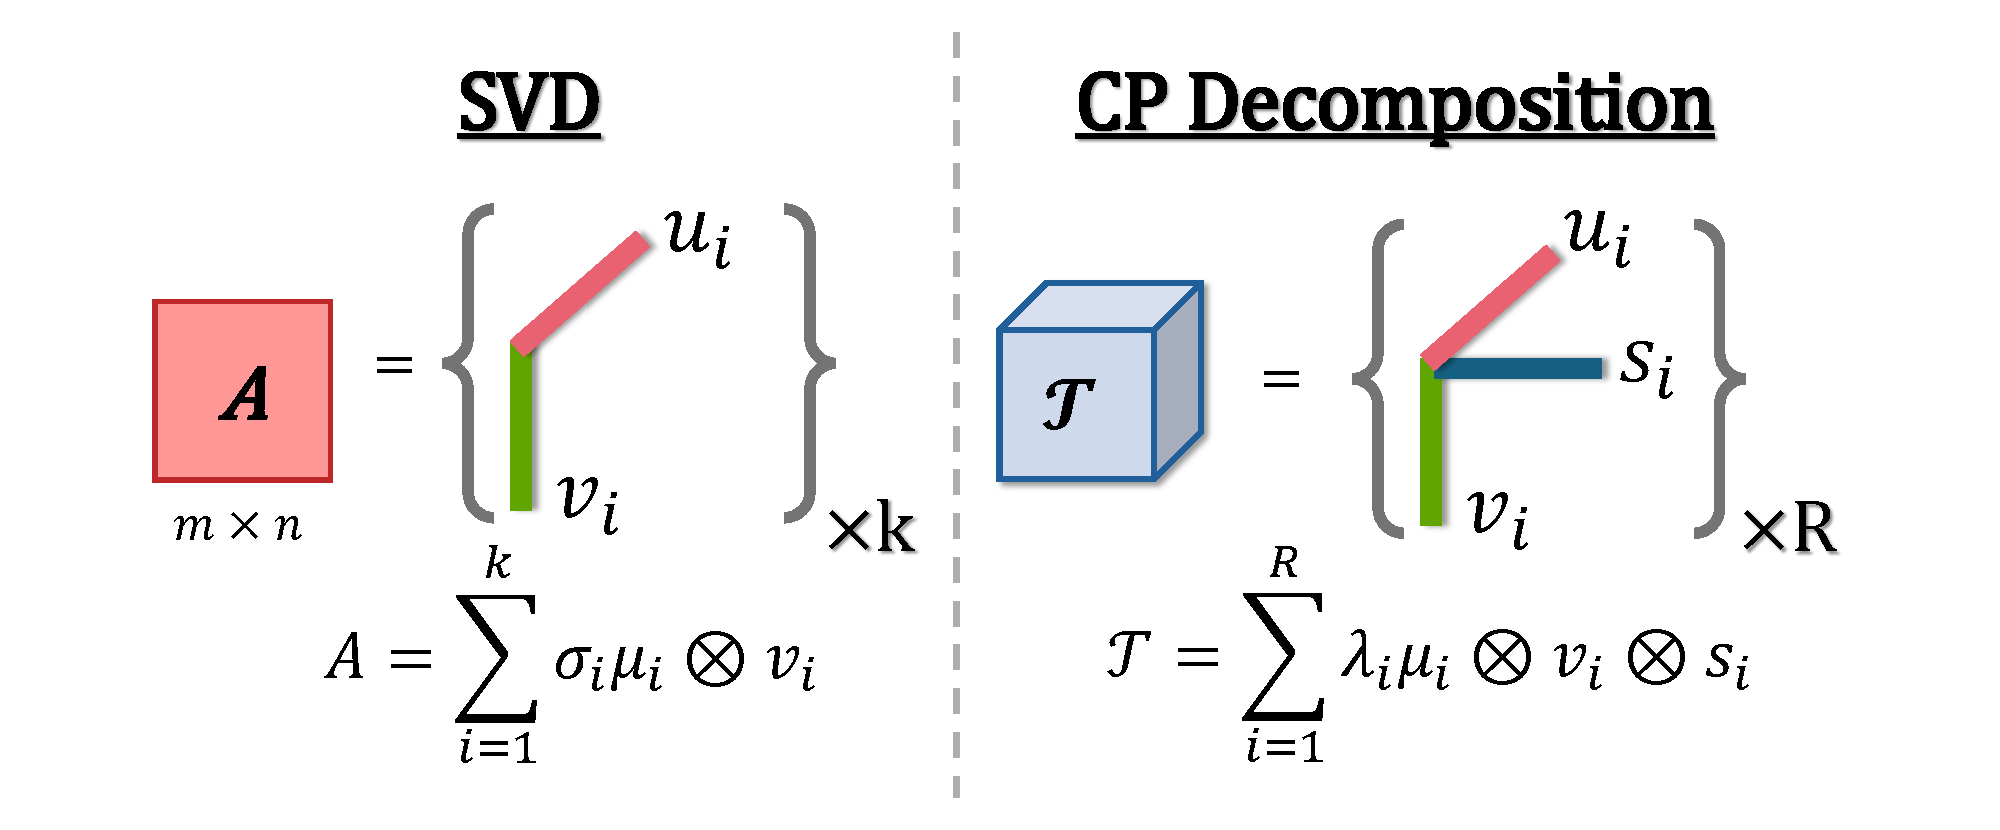
\includegraphics[width=\linewidth]{fig/CP.pdf}
        \caption{An illustration of SVD decomposition of a matrix
        $A\in\mathbb{R}^{m\times n}$ and CP decomposition of third-order tensor
        $\mathcal{T}$.}
        \label{fig:svd_cp}
    \end{wrapfigure}

    To analyze the interplay between multiple LoRA adapters, we leverage the framework of tensor decomposition.  Tensor decomposition aims to approximate a tensor through a set of low-rank
    factors with diverse applications. We specifically focus on the Canonical Polyadic Decomposition (CPD), which was originally introduced by \citet{hitchcock1927expression,hitchcock1928multiple} as a method to represent a tensor as a sum of a minimum number of rank-one tensors. CPD (Fig. \ref{fig:svd_cp})is often considered a special case of the more general Tucker Decomposition \citep{de2000multilinear,tucker1966some}, which decomposes a tensor into a core tensor multiplied by a factor matrix along each mode. While Tucker decomposition offers high flexibility, we utilize CPD in this work because its uniqueness properties—under mild conditions—allow for the identifiable isolation of task-specific information, which is critical for mitigating task interference. In this way, a high-order tensor can be uniquely represented as the
    sum of a set of rank-one tensors. Given a third-order tensor $\mathcal{T}\in\mathbb{R}
    ^{d\times r\times N}$, the CP decomposition is expressed as:
    \begin{equation}
        \label{eq:cp_decomposition}\mathcal{T}=\sum_{i=1}^{R}\lambda_{i}\mathbf{u}
        _{i}\otimes \mathbf{v}_{i}\otimes \mathbf{s}_{i}
    \end{equation}

   
    where $R$ is the rank of CP decomposition. $\lambda_{i}$ is the scaling weight.
    $\mathbf{u}_{i}$, $\mathbf{v}_{i}$ and $\mathbf{s}_{i}$ are the factor vectors
    corresponding to the three modes of $\mathcal{T}$. The operator $\otimes$
    denotes the outer product.


\section{Method}
 \begin{figure*}[htpb]
        \small
        \centering
        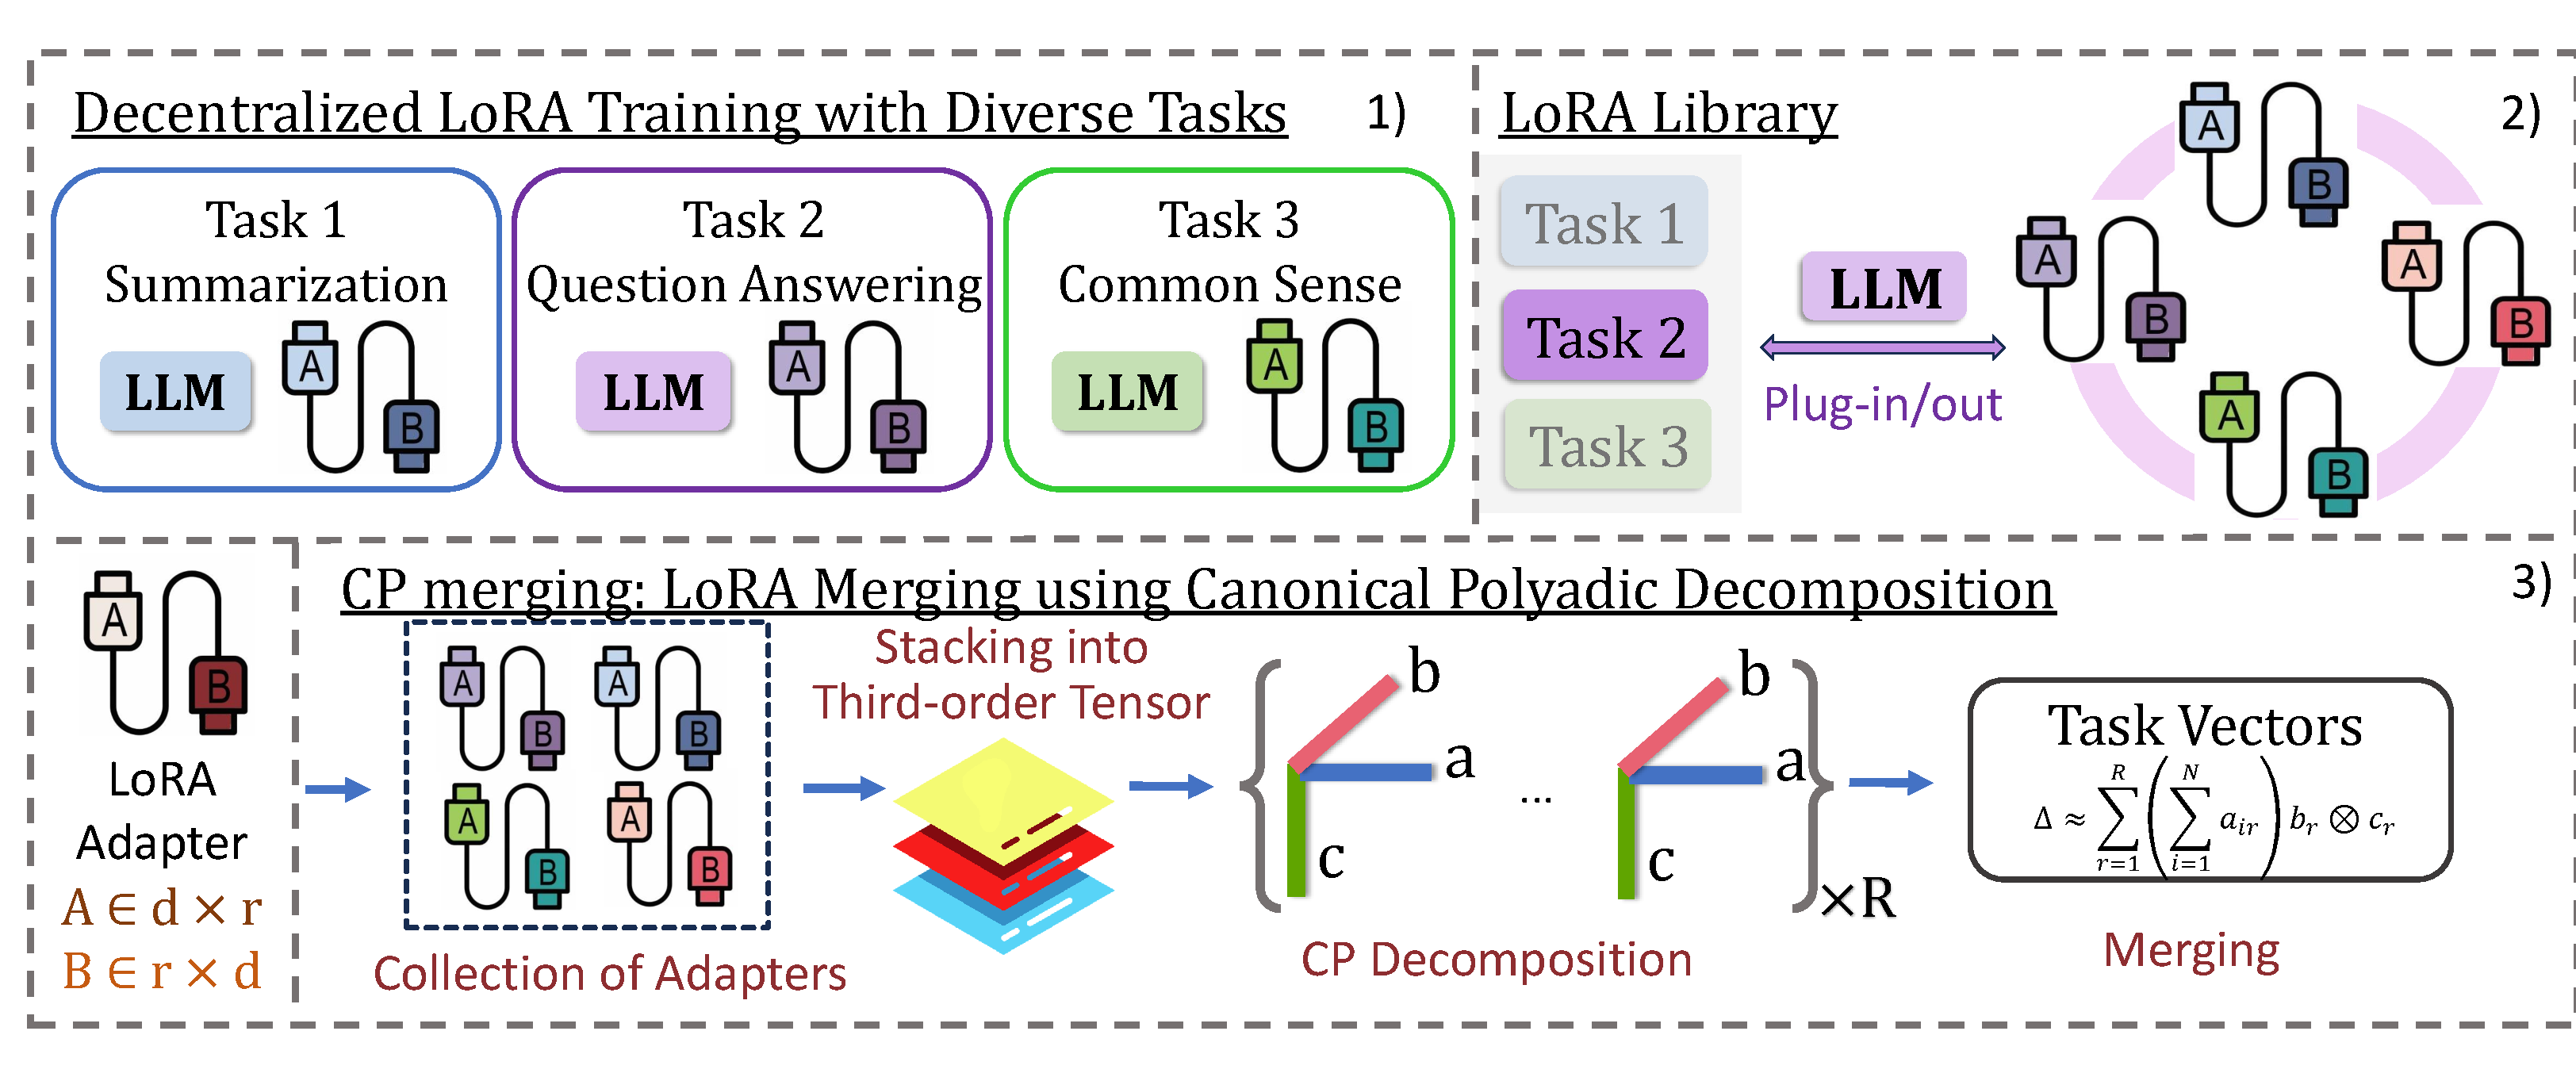
\includegraphics[width=0.99\linewidth]{fig/CP_merging.pdf}
        \caption{1) LoRA adapter from various tasks, each LoRA adapter is
        trained individually. 2) LoRA library aims to leverage the plug-in/out
        nature of LoRAs to offer the ability to add or remove knowledge from
        LLMs. 3) CP merging: we stack the
        LoRA into a third-order tensor and conduct the CP merging.}
        \label{fig:factorizing_lib}
    \end{figure*}
    \subsection{CP Merging}
    \paragraph{Task Singular Vectors}
    \citep{gargiulo2025task} use SVD to decompose the layer task matrices and
    term the obtained singular vectors \textit{Task Singular Vectors (TSV)},
    revealing low-rank properties and deeper insight into the inter-task
    interactions. Given two tasks $i$ and $j$, the tasks matrix $\Delta_{i}$ and
    $\Delta_{j}$ can written as:

    \begin{align}
        \Delta_{i} & = U_{i}\Sigma_{i}V_{i}^{\top}, \quad \Delta_{j}= U_{j}\Sigma_{j}V_{j}^{\top}
    \end{align}

    where $U_{i}$, $U_{j}$ are the left singular vectors and $V_{i}$, $V_{j}$ are
    the right singular vectors. $\Sigma_{i}$,$\Sigma_{j}$ are diagonal matrices
    of singular values. As shown in Fig. \ref{fig:svd_cp}, we can interpret SVD as
    a sum of rank-one matrices. For each task $i$, we get the best approximation
    of each task matrix $\Delta_{i}$ by retaining only the top-$k$ singular values
    and their corresponding vectors:

    \begin{equation}
        \hat{\Delta}_{i}= \sum_{j=1}^{k}\sigma_{j}^{i}\, \mathbf{u}_{j}^{i}\otimes
        {\mathbf{v}_j^i}.
    \end{equation}
    \begin{wrapfigure}[18]{r}{0.50\textwidth}
\vspace{-20pt} 
  \centering
  \begin{minipage}{0.48\textwidth}
    \begin{algorithm}[H]
        \caption{Implementation of CP Merging}
        \algsetup{linenosize=\small} % Adjust line number size
        \begin{algorithmic}[1] % The [1] here means line numbers will be shown starting from 1
            \STATE Input: Pretrained task LoRA adapters$\{\Delta_{1},\Delta_{2},..., \Delta_{N}\}$, scaling factors $\alpha$. 
            \STATE \textbf{Output:
            Merged weight $W_{\mathrm{MT}}$} 
            
            % \STATE $E=[]$ 

            % \FOR{$i = 1$ to $N$} \STATE $\Delta_{i}$=Train($\mathcal{C}_{i}$, LLM)
            % \ENDFOR

            \STATE \textbf{Concatenate} the matrices: \STATE $\mathcal{T}\leftarrow
            [\Delta_{1}|\Delta_{2}|...|\Delta_{N}]$

            \STATE \textbf{CP Decomposition:}

            \STATE
            $\mathcal{T}\approx \sum_{r=1}^{R}\mathbf{a}_{r}\otimes \mathbf{b}_{r}
            \otimes \mathbf{c}_{r}$
            (Eq. \ref{eq:cp_decomposition})

            \STATE \textbf{Compute the Task Matrix:}

            \STATE
            $\Delta_{i}\approx \sum_{r=1}^{R}a_{ir}\textbf{b}_{r}\otimes \textbf{
             c}_{r}$
            \quad\quad (Eq.\ref{eq:cp_form})

            \STATE \textbf{Reconstruct} the merged matrix:

            \STATE $\Delta \approx \sum_{r=1}^{R}\left( \sum_{i=1}^{N}a_{ir}\right
            ) \textbf{b}_{r}\otimes \textbf{c}_{r}$ \quad (Eq.
            \ref{eq:cp_merge})

            \STATE \textbf{Construct} the merged model weights: \STATE
            $W_{\mathrm{merged}}=W_{\text{base}}+\alpha\sum_{r=1}^{R}\left( \sum_{i=1}^{N}a_{ir}\right
            ) \textbf{b}_{r}\otimes \textbf{c}_{r}$
            \STATE \textbf{return} $W_{\mathrm{MT}}$
        \end{algorithmic}
        \label{al:factorizing}
    \end{algorithm}
\end{minipage}
\end{wrapfigure}
    where $\hat{\Delta}_{i}$ is the low-rank approximation of the task matrix
    for task $i$, obtained using the top-$k$ singular values $\sigma_{i,j}$,
    left singular vectors $\mathbf{u}_{i,j}$ and right singular vectors
    $\mathbf{v}_{i,j}$. \texttt{Knots} conduct the SVD decomposition individually to obtain the right singular matrix $[V_1,V_2,...,V_N]$ and then merge the right singular matrix to obtain a merged matrix $V^{(\text{merged})}$. The final task matrix can be computed by: $\ Delta W_{j}^{(\text{merged})} = U\Sigma[V^{(\text{merged})}]^T$. \texttt{TSV merging} decomposes the LoRA adapters individually and then concatenates the left singular matrix $[U_1,U_2,...,U_N]$ and right singular matrix $[V_1,V_2,...,V_N]$. We notice that SVD decomposes the task adapter separately, leading to independent choices of SVD dimensions. To address this, we propose a more general global decomposition 
    using Canonical Polyadic (CP) decomposition, which takes all the LoRAs together as a tensor input. 

    \paragraph{Representing all adapters as a Third-Order Tensor}
    
    We consider the task adapters $\Delta_{i}$ for all tasks $i$ as slices of a
    third-order tensor $\mathcal{T}$, where the dimensions could be interpreted
    as (tasks, input dimension, output dimension). Let use denote this tensor $\mathcal{T}
    \in\mathbb{R}^{d_{in}\times d_{out}\times N}$ where $N$ is the number of tasks,
    $d_{in}, d_{out}$ are the dimensions of each task matrix $\Delta_{i}$. Each $\Delta
    _{i}$ (a matrix of size $d_{in}\times d_{out}$) is a frontal slice of $\mathcal{T}$
    along the task mode. So, we can concatenate the $\Delta_{i}$ matrices along the
    task dimension to form $\mathcal{T}$.

    
    \paragraph{CP Decomposition Form}

    In CP decomposition, the tensor $\mathcal{T}$ is approximated as a sum of rank-one
    tensors:

    \begin{equation}
        \label{eq:cp_decomposition}\mathcal{T}\approx \sum_{r=1}^{R}\lambda_i\mathbf{a}_{r}
        \otimes \mathbf{b}_{r}\otimes \mathbf{c}_{r}
    \end{equation}

    where $R$ is the number of components (analogous to $k$ in SVD), $\mathbf{a}_{r}
    \in \mathbb{R}^{N}$ is a vector associated with the task mode,
    $\textbf{b}_{r}\in \mathbb{R}^{d}_{in}$ and
    $\textbf{c}_{r}\in \mathbb{R}^{d}_{out}$ are vectors associated with the row
    and column modes. In our paper, we set $\lambda_i=1$, For each task $i$, the $i$-th slice $\Delta_{i}$ of
    $\mathcal{T}$ would be:

    \begin{equation}
        \label{eq:cp_form}
        \Delta_{i}\approx \sum_{r=1}^{R}a_{ir}\mathbf{b}_{r}\otimes
        \mathbf{c}_{r}
    \end{equation}

    where $a_{ir}$ is the $i$-th element of $\mathbf{a}_{r}$, selecting the
    contribution of the $r$-th component for task $i$.

    \paragraph{CP merging over the task mode}

    To merge the $\Delta_{i}$ into a final $\Delta$, we sum over the task dimension
    (mode-1). The merged $\Delta$ would be:

    \begin{equation}
        \Delta = \sum_{i=1}^{N}\Delta_{i}\approx \sum_{i=1}^{N}\sum_{r=1}^{R}a_{ir}
        \mathbf{b}_{r}\otimes \mathbf{c}_{r}
    \end{equation}

    Since the outer product $\textbf{b}_{r}\otimes \textbf{c}_{r}$ is the same for
    all $i$, and assuming $a_{ir}$ represents the weight of
    component $r$ for task $i$, we can factorize this as:
    \begin{equation}
        \label{eq:cp_merge}\Delta \approx \sum_{r=1}^{R}\left( \sum_{i=1}^{N}a_{ir}
        \right) \mathbf{b}_{r}\otimes \mathbf{c}_{r}
    \end{equation}

    where $\sum_{i=1}^{N}a_{ir}$ is the total contribution of the $r$-th component
    across all tasks. The final merged weights can be written as :

    \begin{equation}
        W_{\mathrm{MT}}=W_{0}+\sum_{r=1}^{R}\left( \sum_{i=1}^{N}a_{ir}\right) \textbf
        {b}_{r}\otimes \textbf{c}_{r}
    \end{equation}

\section{Experimental Results}

    To test the effectiveness of our approach, we evaluate CP Merging on a
    variety of LoRA merging methods in held-in and held-out multi-tasks based on Flan datasets (Sec. \ref{sec:held_in_out})\cite{arnobexploring,ostapenko2024towards}
    and zero-shot task (Sec. \ref{sec:zero_shot})\cite{ostapenko2024towards} and skill composition tasks (Appendix \ref{sec:skill_composition})\cite{prabhakar2025lora}.

    \paragraph{Baselines}
    We compare the following methods in the zero-shot benchmark. \textbf{BASE}: The
    base model without adaptation. \textbf{Multi-task}: A single expert LoRA
    finetuned on a joint training set. \textbf{Uniform}:
    For each task, we train a LoRA adapter, then we merge the LoRA uniformly
    \citep{huang2023lorahub,chronopoulou2023adaptersoup}. \textbf{Task
    Arithmetic (TA)} \citep{ilharco2022editing} subtracts the parameter values
    of the pre-trained model from those of the fine-tuned models, creating a set
    of "task-vectors." Then they linearly summed to create a merged model.
    \textbf{Ties-merging} \citep{yadav2023ties}: Ties improves TA by resolving the
    parameter interference between models when merging. It prunes low-magnitude
    weights and then only averages the weights that share the dominant sign. \textbf{DARE}
    randomly drops fine-tuned weights and rescales the remaining ones to create
    sparse task vectors \cite{yu2024language}. \textbf{TSV merging} uses SVD decomposition to compress the LoRA and reduce the task interference based on the singular vectors \citep{marczak2025no}.  \textbf{Knots} uses the SVD to transform the weights of jointly
    different LoRA models into a shared space \citet{stoica2025model}. \textbf{ISO-C}
    \cite{marczak2025no} proposes an isotropic merging framework that flattens
    the singular value spectrum of the
    task matrix. 
    \begin{table*}[h]
\small
\centering
\begin{adjustbox}
{width=1.0\textwidth}
\begin{tabular}{l|ccccccccccc|c} 
\Xhline{1.6pt}
\textbf{Model} & \textbf{Wiqa} & \textbf{Sciq} & \textbf{Adver} & \textbf{Duorc} & \textbf{Cos} & \textbf{Wikiqa} & \textbf{Quail} & \textbf{Wikihop} & \textbf{ParaphQa} & \textbf{Yelp} & \multicolumn{1}{c}{\textbf{AVG}} & \textbf{3 Held-Out} \\
\midrule

\rowcolor{lightgray}\multicolumn{13}{c}{\textbf{Phi-3 (3B) with LoRA library }} \\
\textbf{BASE} & 14.55 & 7.99 & 10.85 & 7.32 & 5.00 & 4.17 & 11.88 & 3.51 & 6.93 & 8.33 & \cellcolor[HTML]{FDE9E8} 8.05 & \cellcolor[HTML]{FDE9E8}  16.00 \\ 
\textbf{Oracle} & 36.87 & 79.56 & 51.58 & 52.40 & 42.99 & 55.94 & 51.51 & 46.58 & 8.325 & 32.71 & \cellcolor[HTML]{FDE9E8}45.85 & \cellcolor[HTML]{FDE9E8}- \\
% \textbf{Multi-task}   & &\cellcolor[HTML]{FDE9E8} & \\

\midrule
\textbf{Uniform} & 22.98 & 61.97 & 29.61 & 18.45 & 28.12 & 11.56 & 38.94 & 7.194  & 7.18 & 15.66  & \cellcolor[HTML]{FDE9E8}24.17 & \cellcolor[HTML]{FDE9E8}\textbf{61.13}\\

\textbf{Ties-merging} & 23.33 & 51.52 & 30.15 & 18.05 & 30.12 & 12.54 & 35.05 & 10.03 & 5.80 & 16.76 & \cellcolor[HTML]{FDE9E8}23.34 & \cellcolor[HTML]{FDE9E8}34.69\\

\textbf{Ties w/DARE} & 25.42 & 52.76 & 32.34 & 19.04 & 31.20 & 13.33 & 36.05 & 7.05 & 6.08 & 16.00 & \cellcolor[HTML]{FDE9E8}23.93 & \cellcolor[HTML]{FDE9E8}34.70\\

\textbf{ISO-C} & 14.59 & 8.19 & 11.11 & 7.50 & 5.38 & 4.20 & 12.23 & 3.53 & 6.95 & 8.39 & \cellcolor[HTML]{FDE9E8}8.20 & \cellcolor[HTML]{FDE9E8}16.18\\
\textbf{TSV Merging} & 36.75 & 53.52 & 44.39 & 20.20 & 59.13 & 23.20& 37.25 & 34.70 & 4.78 & 34.95 & \cellcolor[HTML]{FDE9E8}34.89 & \cellcolor[HTML]{FDE9E8}45.70\\
\textbf{Knots} & 26.33 & 90.81 & 40.15 & 28.87 & 50.44 & 48.35 & 43.24 & 13.71 & 6.63 & 23.56 & \cellcolor[HTML]{FDE9E8}\underline{37.21} & \cellcolor[HTML]{FDE9E8}54.46\\

\midrule

\textbf{CP Merging} & 34.69 & 89.88 & 44.32 & 31.59 & 66.82 & 50.34 & 45.49 & 10.73 & 5.90 & 24.23 & \cellcolor[HTML]{FDE9E8}\textbf{40.40} & \cellcolor[HTML]{FDE9E8}\underline{60.15} \\

\midrule

\Xhline{1.6pt}
\end{tabular}
\end{adjustbox}
\caption{10 held-in and 3 held-out Flan tasks based on Phi-3 3B model. We report the Rouge-L scores. The oracle here denotes that we use the trained LoRA to test the corresponding tasks, which achieve the best results for held-in results. The task details are presented in Appendix \ref{sec:10_held_in}. }
\label{tab:in_domain_full}
\end{table*}
    \subsection{Held-In and Held-out Multi-Tasks}
    \label{sec:held_in_out}

    We conduct our experiments using the FLAN dataset \citep{longpre2023flan} and
    sample 10 held-in and 3 held-out tasks following \citep{ostapenko2024towards,arnob2025exploring}.
    Each task is sub-sampled to 10,000 examples. Within these samples, 1,000 are
    allocated for validation and early stopping.

   
    \begin{wrapfigure}[15]{r}{0.5\textwidth}
    \vspace{-15pt} 
        \small
        \centering
        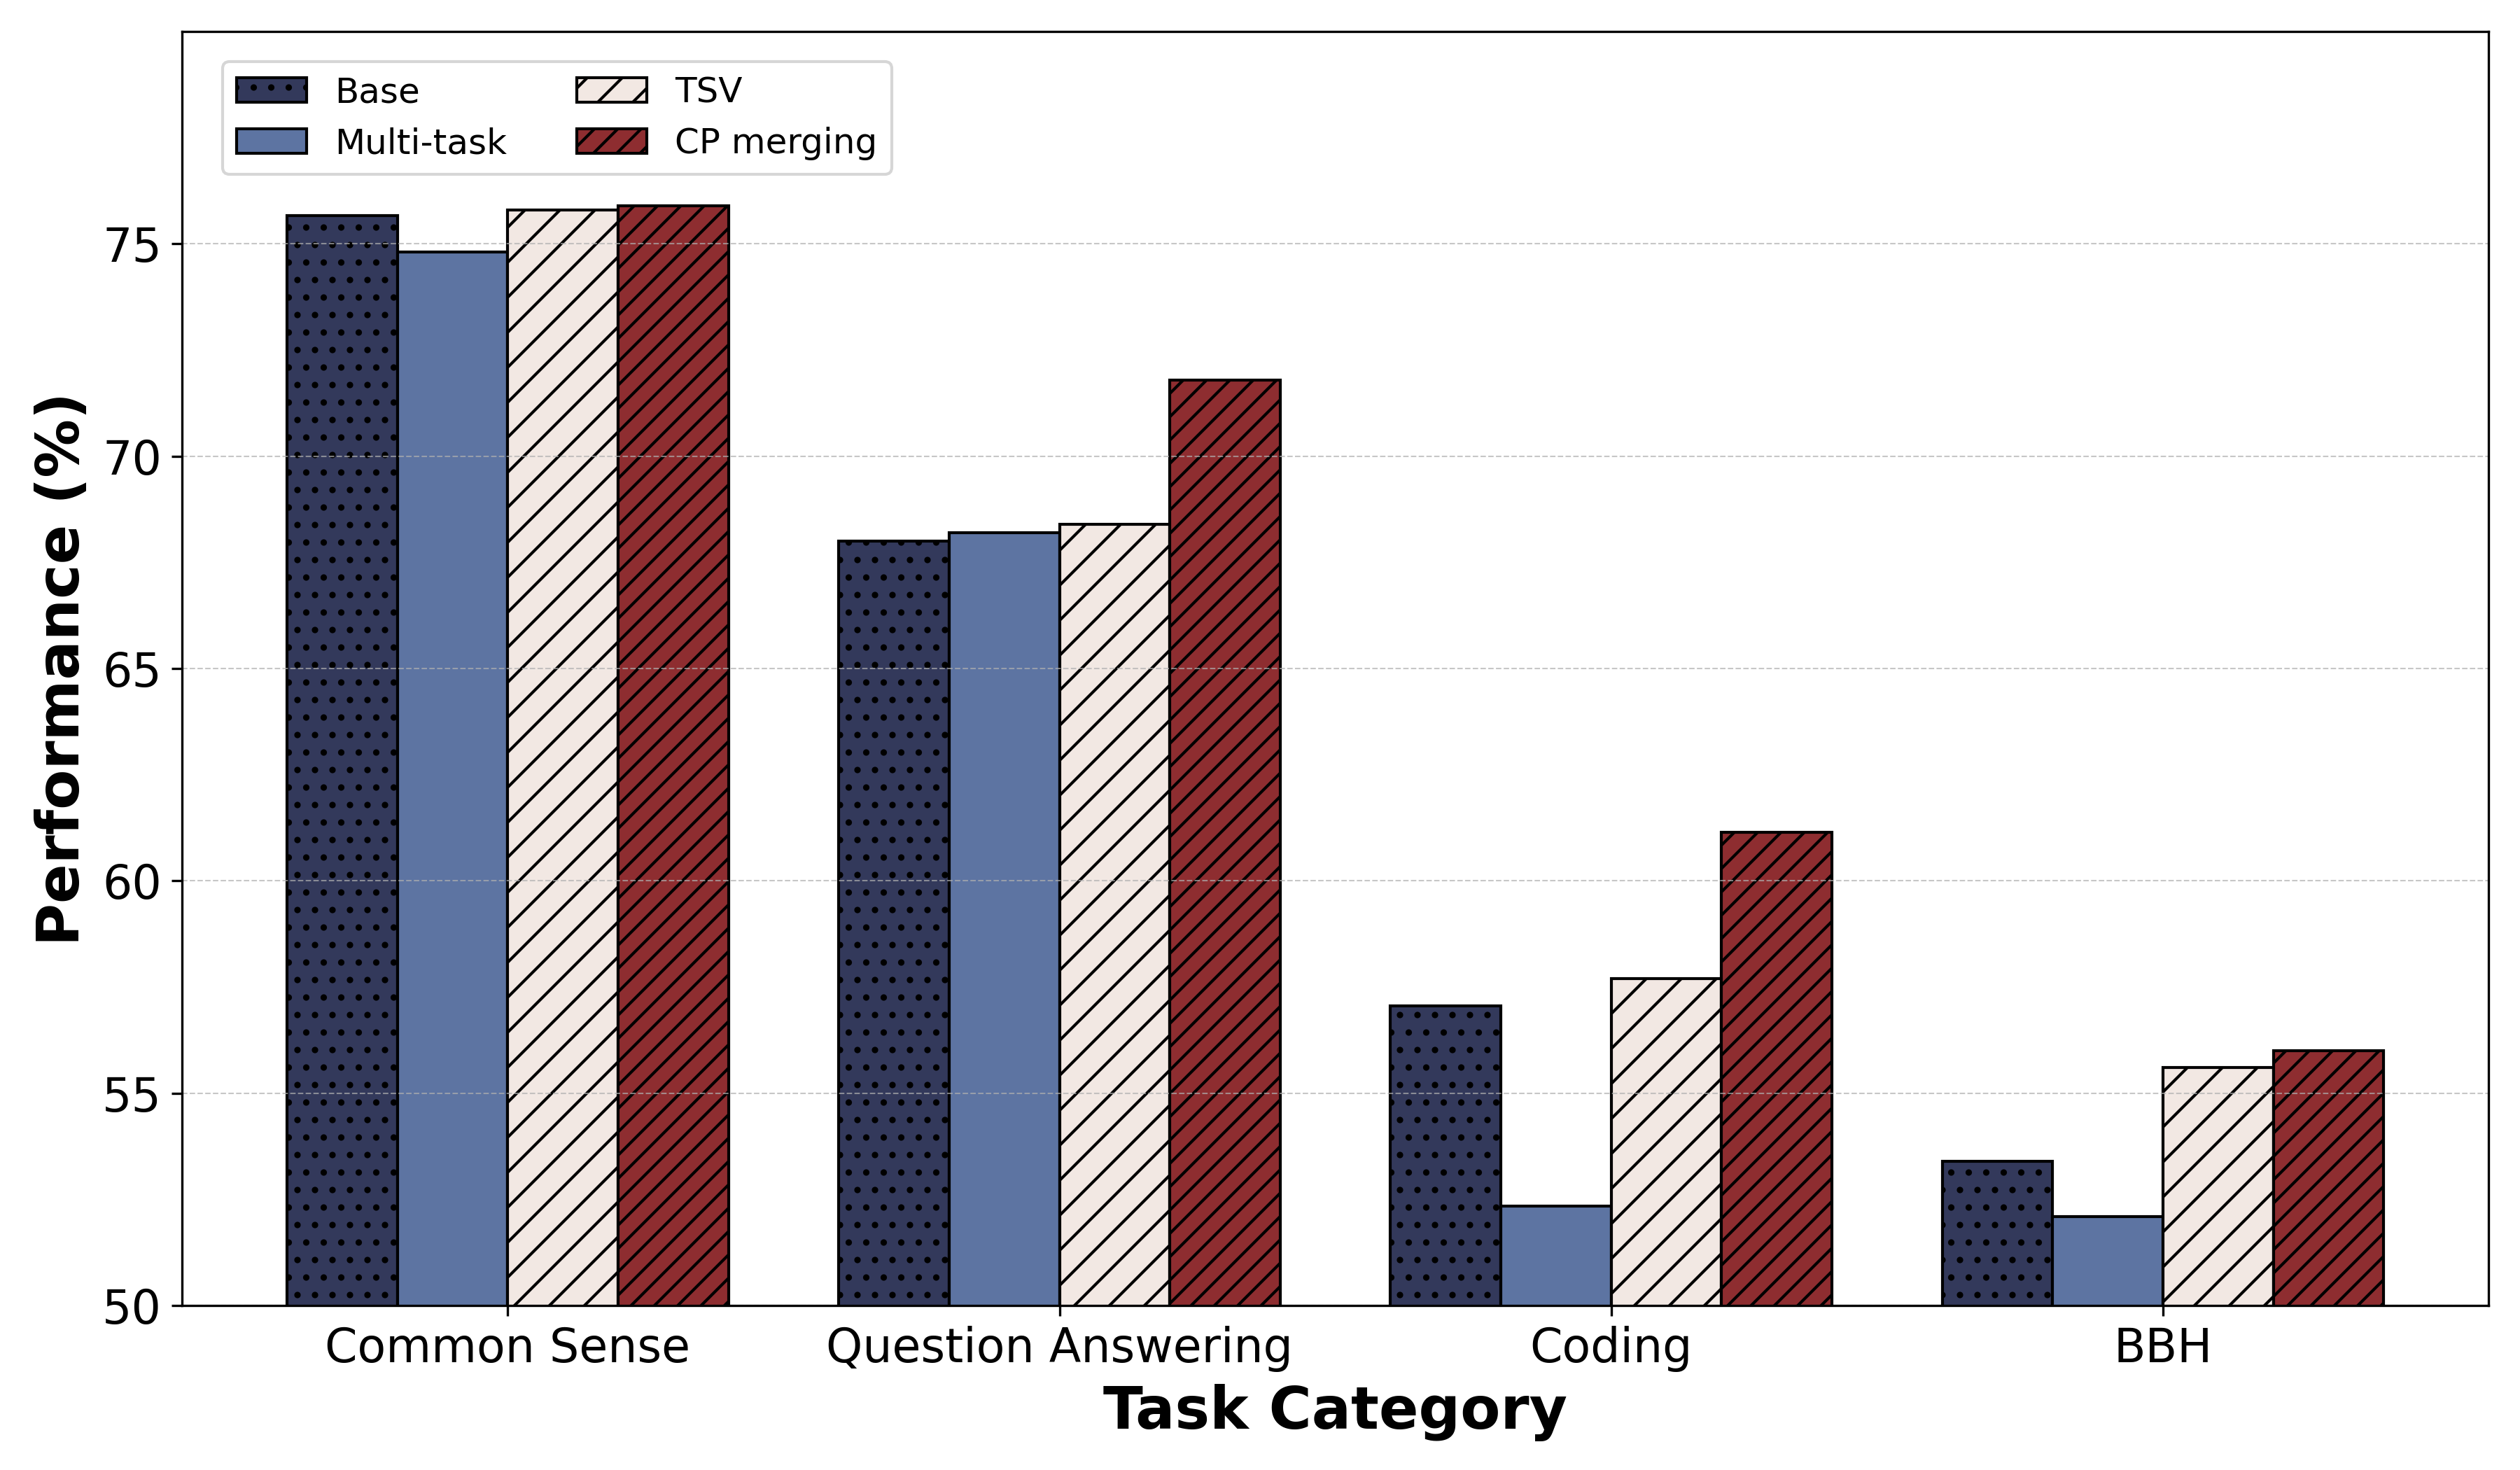
\includegraphics[width=0.50\textwidth]{fig/zero-shot-performance_category_swapped_axes.png}
        \caption{Zero-shot results across different categories. The X-axis represents
        the task categories.}
        \label{fig:performance_categories}
    \end{wrapfigure}
    As shown in Tab. \ref{tab:in_domain_full}. The CP Merging method achieves the highest average score of 40.40, indicating it generally performs best across the tested datasets. It also has a strong 3-Held-Out score of 60.15. CP Merging is the standout performer, showing significant gains over other methods, especially in the average score and the 3-Held-Out evaluation. The BASE model provides a baseline performance, while the Oracle provides an upper bound, representing the theoretical maximum performance without any merging techniques. Ties-merging and Ties w/DARE show similar average performance (23-24). ISO-C has a significantly lower average score, similar to the BASE model's performance. TSV Merging and Knots show moderate performance, with Knots having a higher average score and a much higher 3-Held-Out score. In short, the CP Merging method appears to be the most effective overall, while Uniform merging excels on the specific 3-Held-Out evaluation. 

    \subsection{Zero-shot Experiments}
    \label{sec:zero_shot}
    \begin{table*}[ht]
\small
\centering
\begin{adjustbox}
{width=1.0\textwidth}
\begin{tabular}{l|cccccccccc|c} 
\Xhline{1.6pt}
\multicolumn{1}{c|}{} & \multicolumn{3}{c}{\textbf{Common Sense}} & \multicolumn{4}{c}{\textbf{Question Answering}} & \multicolumn{2}{c}{\textbf{Coding}} & \multicolumn{1}{c}{\textbf{ Reasoning}} & \multicolumn{1}{c}{\textbf{AVG}} \\
\cmidrule(lr){2-4}  \cmidrule(lr){5-8} \cmidrule(lr){9-10}
\cmidrule(lr){11-11}
\multicolumn{1}{c|}{} & \textbf{Piqa} & \textbf{Wg} & \textbf{Hswag} & \textbf{Boolq} & \textbf{Obqa} & \textbf{ArcE} & \textbf{ArcC} & \textbf{HE} & \textbf{Mbpp} & \textbf{BBH} & \multicolumn{1}{c}{\textbf{AVG}} \\
\midrule

\rowcolor{lightgray}\multicolumn{12}{c}{\textbf{Phi-3 (3B) with LoRA library }} \\
\textbf{BASE} & 81.1 & 70.2 & 75.7 & 85.0 & \textbf{49.0} & 80.0 & 57.9 & 53.0 & 61.1 & 53.4 & \cellcolor[HTML]{FDE9E8}66.6\\ 

\textbf{Multi-task}   & 79.1&69.6&75.6&87.1&47.6&82.6&55.6&51.8&52.9& 52.1 &\cellcolor[HTML]{FDE9E8}65.4 \\

\textbf{Uniform} & 81.0&70.4&76.0&84.7&48.8&82.4&57.9&52.4&63.0&55.6&\cellcolor[HTML]{FDE9E8}67.2\\

\textbf{Ties-merging} & 80.8 & \textbf{70.9} & 75.4 & 80.8 & 46.0 & 85.8 & 60.8 & 54.9 & 61.5 & 51.9 & \cellcolor[HTML]{FDE9E8}66.9 \\
\textbf{Task Arithmetic} & 81.0 & 70.5 & 75.9 & 84.7 & 48.8 & 82.5 & 58.2 & 54.3 & 61.9 & 54.2 & \cellcolor[HTML]{FDE9E8}67.2\\
\textbf{Ties w/DARE} & 80.7 & 70.8 & 75.2 & 82.8 & 46.3 & 84.8 & 60.9 & 54.9 & 61.6 & 52.0 & \cellcolor[HTML]{FDE9E8}67.0  \\
\textbf{TA w/DARE} & 81.2 & 70.1 & 75.3 & 84.9 & 48.9 & 82.2 & 58.3 & 54.5 & 61.1 & 54.3 & \cellcolor[HTML]{FDE9E8}67.1 \\
\textbf{TSV Merging} & 81.1 & 70.8 & 75.8 & 86.0 & \textbf{49.0} & 84.3 & 60.4 & 55.0 & 61.2 & 54.0 & 67.7\cellcolor[HTML]{FDE9E8}\\
\midrule
\rowcolor{lightgray}\multicolumn{12}{c}{\textbf{Phi-3 (3B) with C-LoRA library }} \\
\textbf{Uniform} & 81.5 & 69.5 & 76.0 & 86.6 & 48.8 & 86.7  & 61.8 & 57.3  & 65.3 & 55.9  & \cellcolor[HTML]{FDE9E8}\underline{68.9} \\
\textbf{Knots} & 80.8 & 71.7 & 74.9 & 85.0 & 48.0 & 84.1 & 58.2 & 53.2 & 62.6 & 50.4 & \cellcolor[HTML]{FDE9E8}66.9 \\
\textbf{TSV Merging} & 81.3 & 69.3 & 75.6 & 86.4 & 48.8 & 86.1 & 62.3 & 52.4 & 63.3 & 55.1 & \cellcolor[HTML]{FDE9E8}68.1\\
% \textbf{Core merging} \\
\textbf{CP merging} & \textbf{81.7} & 70.0 & \textbf{76.0} & \textbf{86.6}  & 48.9 & \textbf{86.7} & \textbf{62.5}& \textbf{57.3}  & \textbf{65.4} & \textbf{56.0}  & \cellcolor[HTML]{FDE9E8}\textbf{69.1}  \\

\midrule


\Xhline{1.6pt}
\end{tabular}
\end{adjustbox}
\caption{Zero-shot accuracy on 10 downstream benchmarks with Phi-3 (\texttt{microsoft/Phi-3-mini-4k-instruct}). C-LoRA is a LoRA library built by clustering instruction embeddings (Appendix~\ref{sec:clora}). Results with Mistral-7B are in Appendix~\ref{sec:zero_shot_mistral}, and the experimental setting is in Appendix~\ref{sec:exp_setting}.}
\label{tab:zeroshot_full}
\end{table*}

    To test the out-of-domain generalization, we evaluate CP Merging on a variety
    of zero-shot task benchmarks. Specifically, we experiment with four broad
    classes of zero-shot tasks: (1) \textbf{Common Sense Reasoning}: WinoGrande \citep{sakaguchi2021winogrande},
    HellaSwag \citep{zellers2019hellaswag}, and PIQA \citep{bisk2020piqa}. 2)
    \textbf{Question Answering}: BoolQ \cite{clark2019boolq}, OpenbookQA \cite{mihaylov2018can},
    ARC-easy \cite{clark2018think}, and ARC-challenge \cite{clark2018think}. 3) \textbf{Coding}:
    HumanEval \cite{chen2021evaluating}, MBPP \cite{austin2021program}. 4)
    \textbf{General-Purpose Reasoning}: BBH \citep{suzgun2023challenging}.

    \subsubsection{Experimental results}

 

    Tab. \ref{tab:zeroshot_full} presents the average zero-shot accuracy results
    across 10 downstream tasks. The multi-task based on the Phi-3 model (65.4\%)
    underperforms the base model (66.6\%), indicating that the multi-task
    training may encounter \textit{catastrophic forgetting} issue that newly learned
    parameters overwrite or interfere with knowledge acquired during prior training
    \citep{wang2024comprehensive}. LoRA library with uniform merging, consisting
    of 256 experts,  achieves accuracies of 67.2\% for Phi-3. 



    Compared to the C-LoRA library, TSV Merging and Knots are comparable in overall performance. TSV Merging has an average score of 68.1, slightly better than Knots' average of 66.9. While TSV Merging and Knots perform well in some tasks, they do not consistently achieve the top scores that CP merging does. For example, TSV Merging ties for the highest score in Obqa (49.0), but its overall performance is less dominant. CP merging consistently shows superior performance. It achieves the highest average score of 69.1, outperforming all other methods. The results clearly demonstrate the effectiveness of CP merging, which consistently outperforms the other methods, including Knots and TSV Merging. With the highest average score and leading performance in multiple specific tasks, CP merging shows a more robust and effective approach to merging LoRA adapters, successfully mitigating task interference and enhancing overall model performance.

    We further analyze performance across different task categories (Fig. \ref{fig:performance_categories}).
    CP merging improves over the LoRA library with TSV merging, with the largest gains observed in question answering and coding tasks. In contrast,
    improvements on common‑sense reasoning are minimal, suggesting that the impact
    of task interference varies by task type.

\section{Ablation Studies}

    % To investigate the reasons behind the observed improvements, we conducted further analysis.  As previously mentioned, the CP rank $R$ is a critical hyperparameter in CP decomposition. Analyzing $R$ allows us to identify the most impactful components, so we examine the influence of CP rank on performance (Sec. \ref{sec:rank_analyse}). Furthermore, we study the number of clustering approaches (Sec. \ref{sec:clustering}). We also study how CP merging can
    % reduce task interference in \textit{parameter-level} (Sec. \ref{sec:cp_merging}). Lastly, we analyze the memory requirements of different library approaches (Sec. \ref{sec:memory_usage}).

    % \begin{figure}[h]
    %     \centering
    %     \includegraphics[width=\linewidth]{fig/common-sense.png}
    %     \caption{Comparison of our approaches on Common-sense
    % reasoning tasks. We present all the results based on Phi-3.}
    %     \label{fig:common_sense_reasoning}
    % \end{figure}

    % \begin{figure}[h]
    %     \centering
    %     \includegraphics[width=\linewidth]{fig/coding.png}
    %     \caption{Comparison of our approaches on Coding
    % tasks. }
    %     \label{fig:coding}
    % \end{figure}

    


\subsection{Number of Tasks analysis}


Overall, the merging methods significantly outperformed the Base model across all task sizes. The Base model consistently showed the lowest ROUGE-L scores, with scores of 11.14, 9.15, and 8.05 for 3, 5, and 10 tasks, respectively. This suggests that LoRA merging is an effective technique for improving performance. 
CP consistently delivered the best performance on ROUGE-L scores. For 5 tasks, TSV merging and Knots merging performed equally well, both achieving a score of 54.4. The CP merging method surpasses Knots merging with a score of 57.7 for this task size. For 10 tasks, both the Knots and TSV merging methods saw a considerable drop in performance. In contrast, the CP merging method demonstrated superior robustness to an increase in the number of tasks, achieving the highest score of 40.40 in this category. The results indicate that LoRA merging is a highly effective strategy for improving model performance on multiple tasks. Specifically, the CP merging method shows the most promise, as it consistently achieves top-tier performance and exhibits greater stability as the number of tasks increases. 
\begin{table}[h]
    \centering
    \begin{tabular}{l|ccc}
    \toprule
      Model  & 3 tasks & 5 tasks & 10 tasks \\
    \midrule
     Base    & 11.14 & 9.15 & 8.05\\
     TSV merging & 44.87 & 54.4 & 34.89\\
     Knots & 59.04 & 54.4& 37.21\\
     \midrule
     CP merging & \textbf{59.06} & \textbf{57.7} & \textbf{40.40}\\
     \bottomrule
    \end{tabular}
    \caption{The influence of the task size for LoRA merging. We select 3, 5, and 10 tasks from the Flan datasets and report the average Rouge-L scores for all the tasks.}
    \label{tab:tasks_size}
\end{table}



\subsection{CP Merging for Task Interference} 
\label{sec:cp_merging}


% \begin{wrapfigure}[13]{r}{0.5\textwidth}
% \vspace{-20pt}
% \centering
% 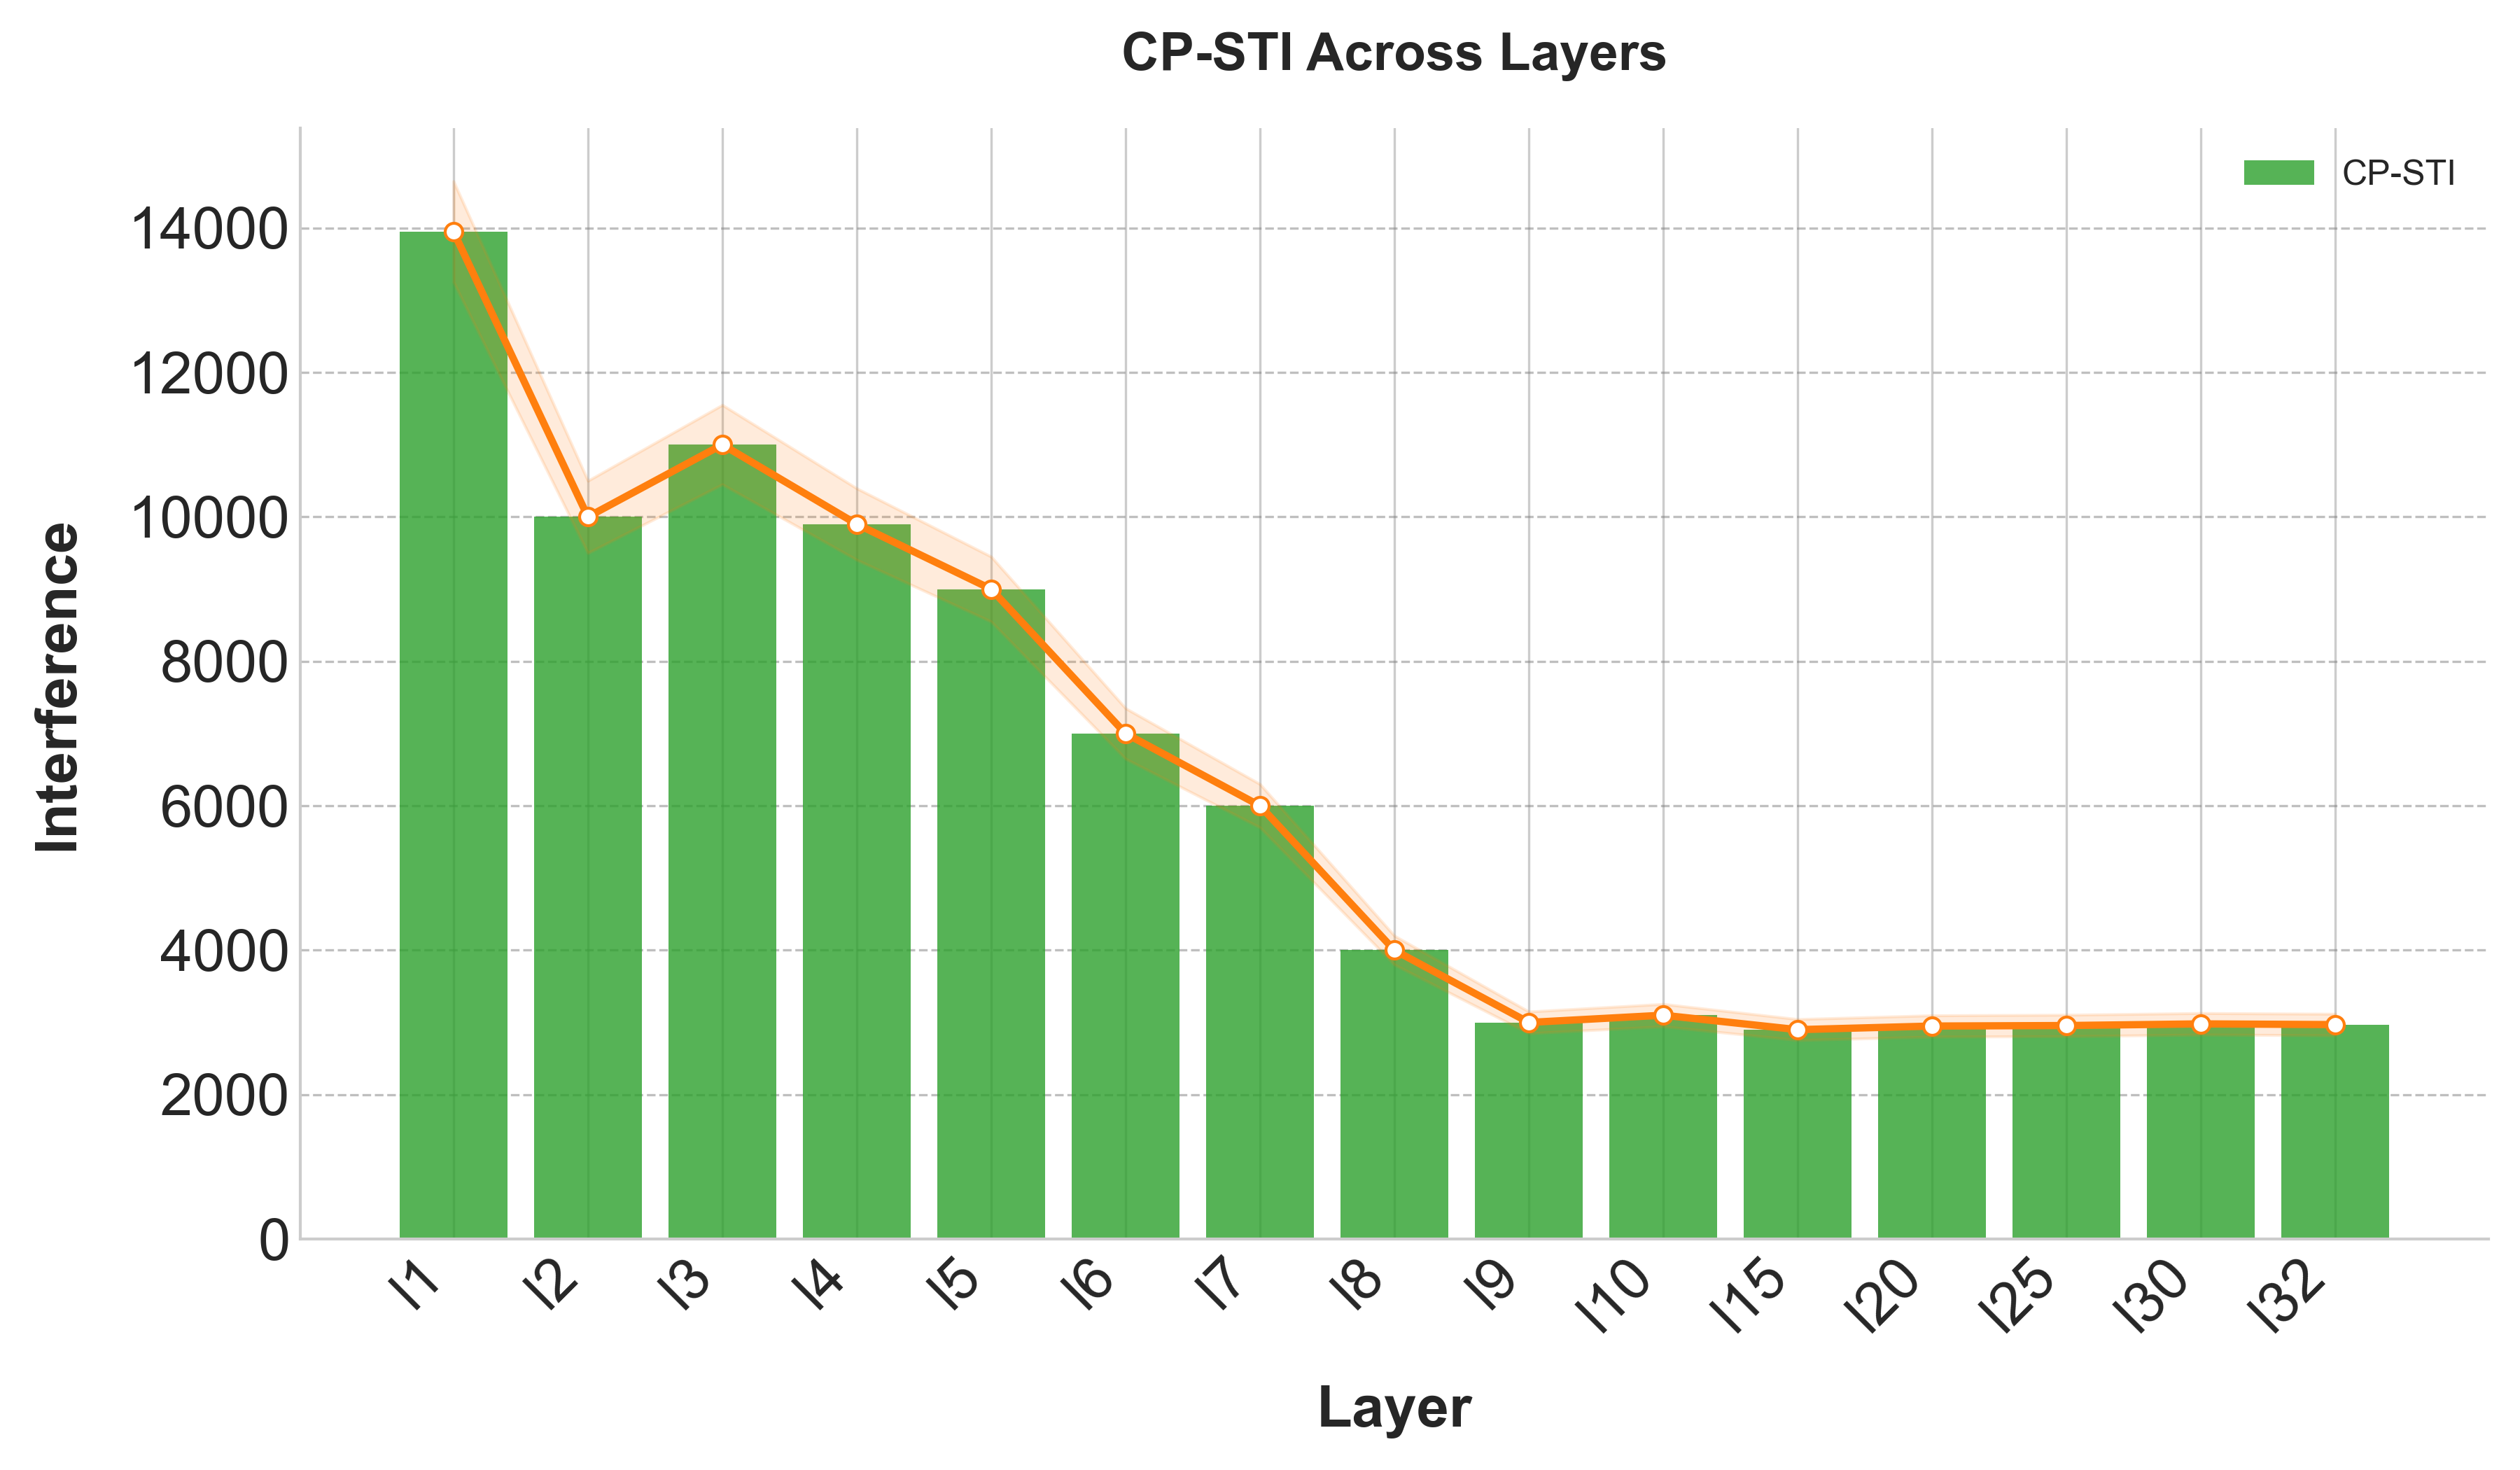
\includegraphics[width=0.5\textwidth]{fig/cp_sti_across_layers.png}
% \caption{CP-STI across layers in the LLama 7B for Math and Code LoRA.}
% \label{fig:cp_str_interference}
% \end{wrapfigure}

To study the task interference,  \cite{gargiulo2025task} introduces a score of task interference (termed as \textit{Singular Task Interference}) based on the interplay of TSVs from different tasks:

\begin{equation}
    \textbf{STI}\left( \left\{ \Delta_i \right\}_{i=1}^{N} \right) 
= \left\| \left( U^\top U - I \right) \Sigma \left( V^\top V - I \right) \right\|_1
\end{equation}

They assume that higher inner product values for $U^TU$ and $V^TV$ imply a higher likelihood \citep{gargiulo2025task}. The intuition is that overlapping singular vectors suggest shared features in the weight space across tasks. Inspired by this, we can reformulate the STI with CP decomposition. To define a CP-based STI metric, we need to assess the interference caused by the interplay of these factor matrices across tasks. The intuition remains that overlapping components (shared features in the weight space) lead to interference when merged. We can adapt the STI by considering the alignment and orthogonality of the factor matrices $a_r$, $b_r$, and $c_r$ across tasks. Then we define the CP-based Singular Task Interference (CP-STI) as:




\begin{figure}[h]
    \centering
    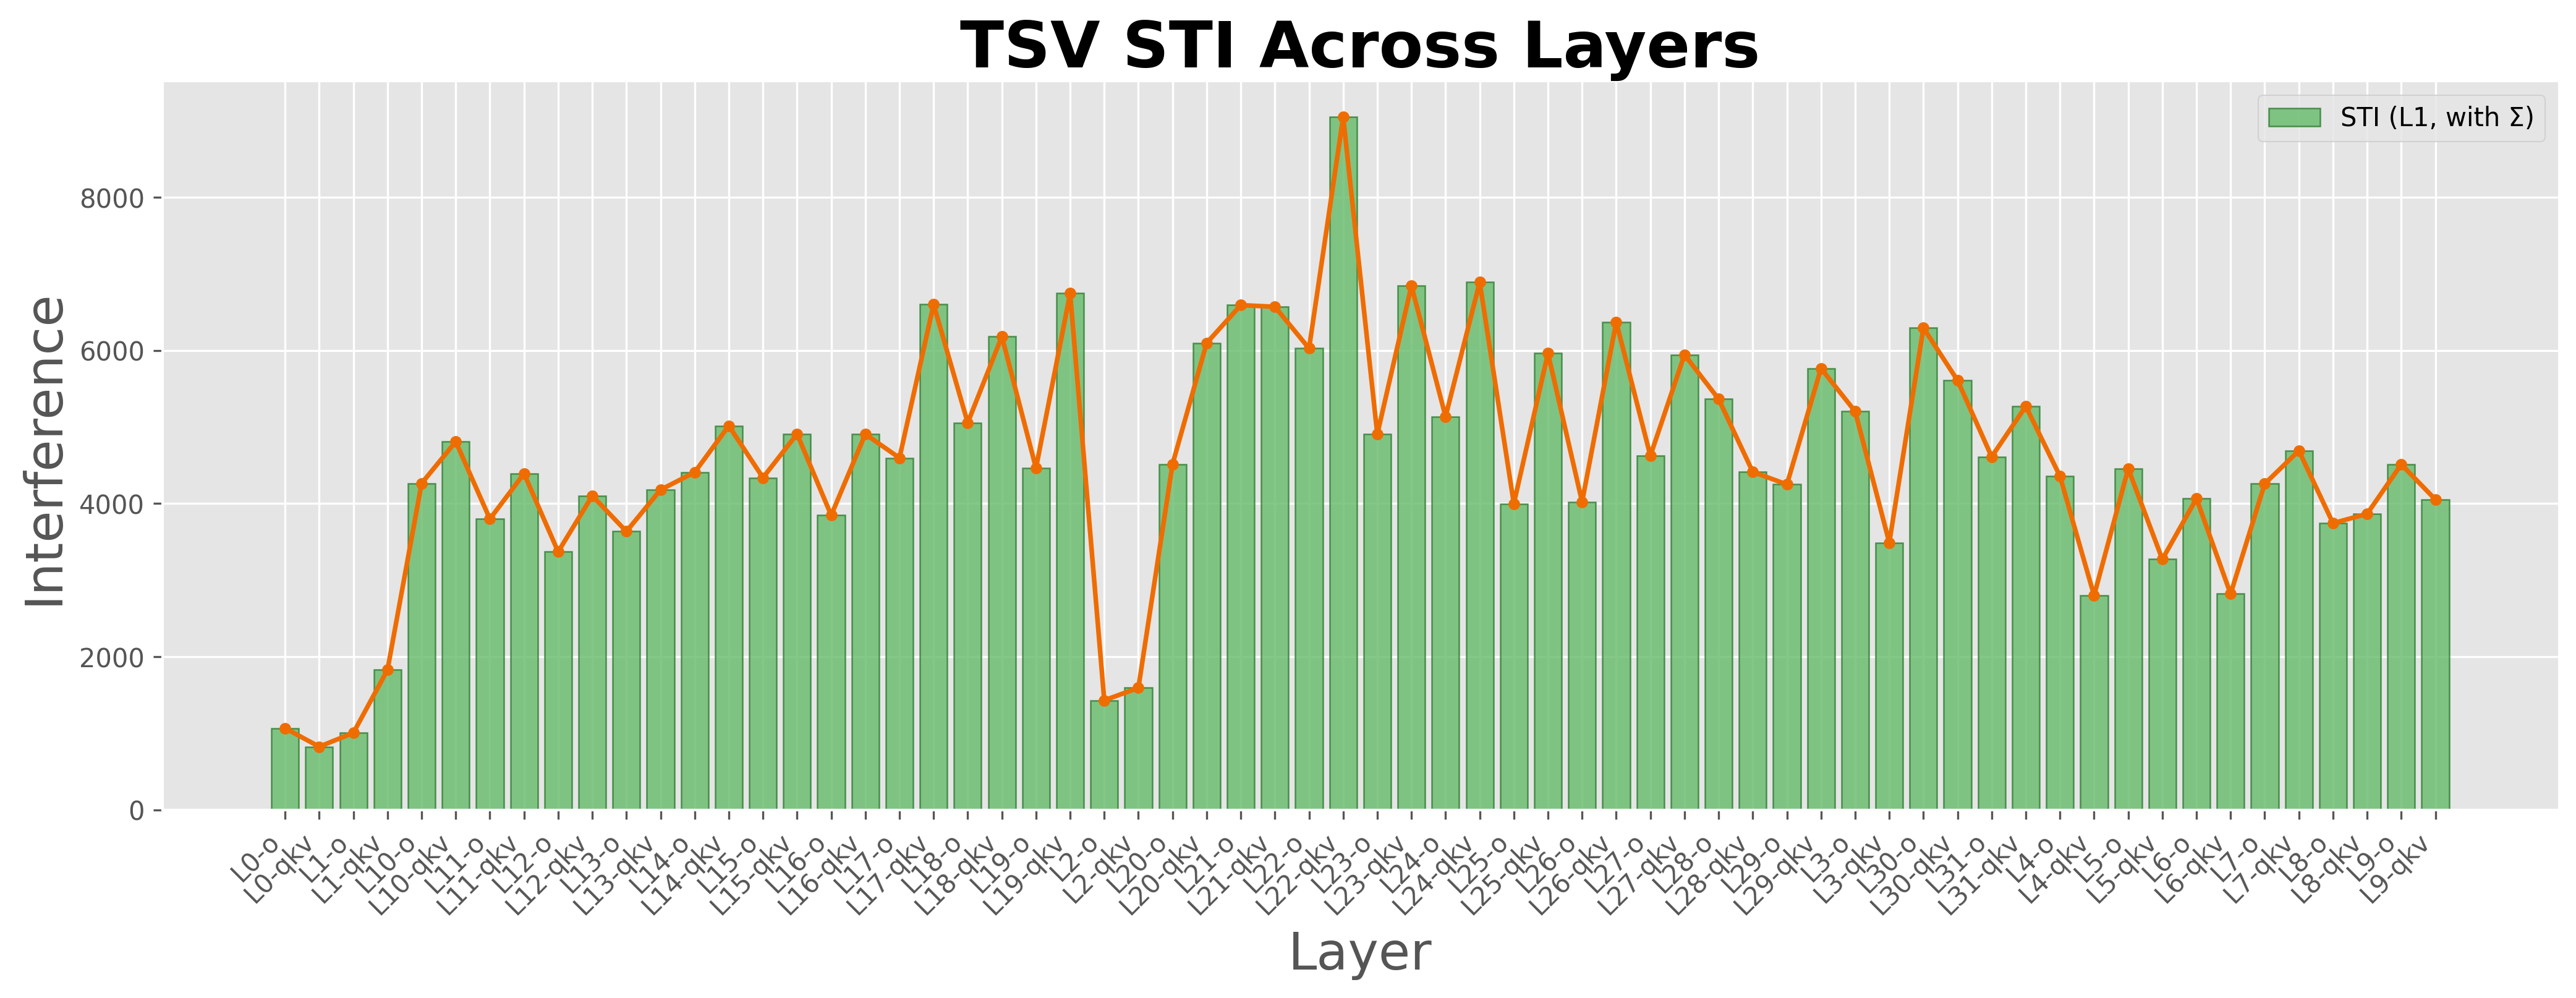
\includegraphics[width=0.7\linewidth]{fig/tsvmerge_sti_across_layers_beautified.png}
    \caption{STI evaluation in TSV across layers based on 5 flan tasks.}
    \label{fig:sti}
\end{figure}
where $A=[a_1, a_2, \ldots, a_R] \in \mathbb{R}^{N \times R}$ is the matrix formed by stacking the task-mode factor vectors $a_r$, $B=[b_1, b_2, \ldots, b_R] \in \mathbb{R}^{d \times R}$ is the matrix of row-mode factors, $C= [c_1, c_2, \ldots, c_R] \in \mathbb{R}^{d \times R}$ is the matrix of column-mode factors, $\circ$ denotes the Hadamard (element-wise) product, $I$ is the identity matrix of appropriate dimension (e.g., $R \times R$). Overlapping factors (high inner products) suggest shared features across tasks, which can introduce interference when the decomposed representations are merged, potentially degrading individual task performance.

\begin{equation}
\label{eq:cp_sti}
  \mathbf{CP-STI}(\{\Delta_i\}_{i=1}^N) = \|(A^T A - I) \circ (B^T B - I) \circ (C^T C - I)\|_1
\end{equation}

\begin{figure}
    \centering
    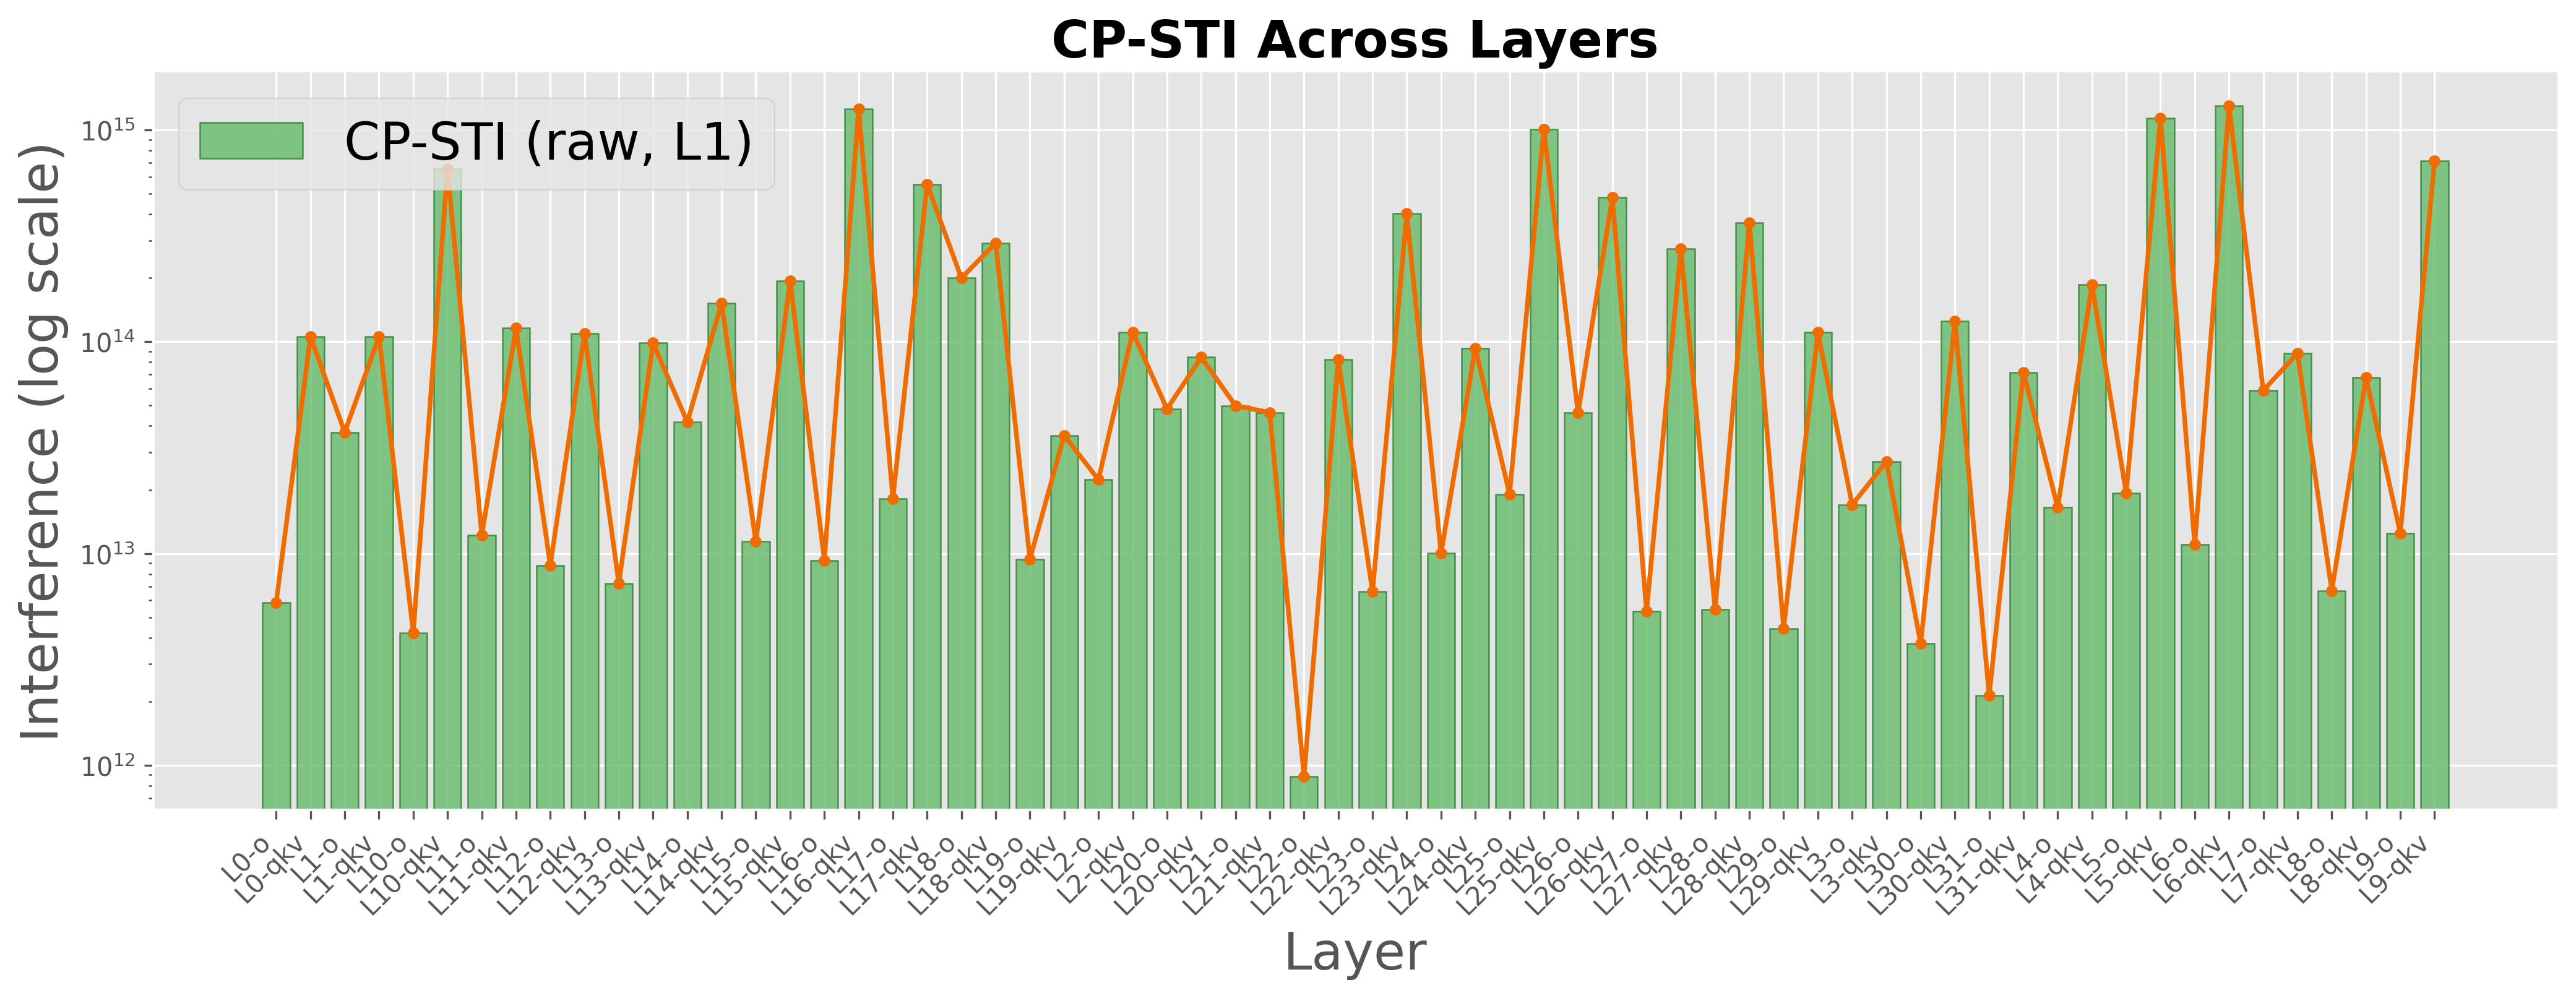
\includegraphics[width=0.7\linewidth]{fig/cpmergeafter_cp_sti_across_layers_beautified.png}
    \caption{CP-STI evaluation in CP merging across layers based on 5 flan tasks.}
    \label{fig:cp_sti}
\end{figure}



% \begin{figure}[h]
%         \centering
%         \begin{subfigure}
%             {0.45\textwidth}
%             \centering
%         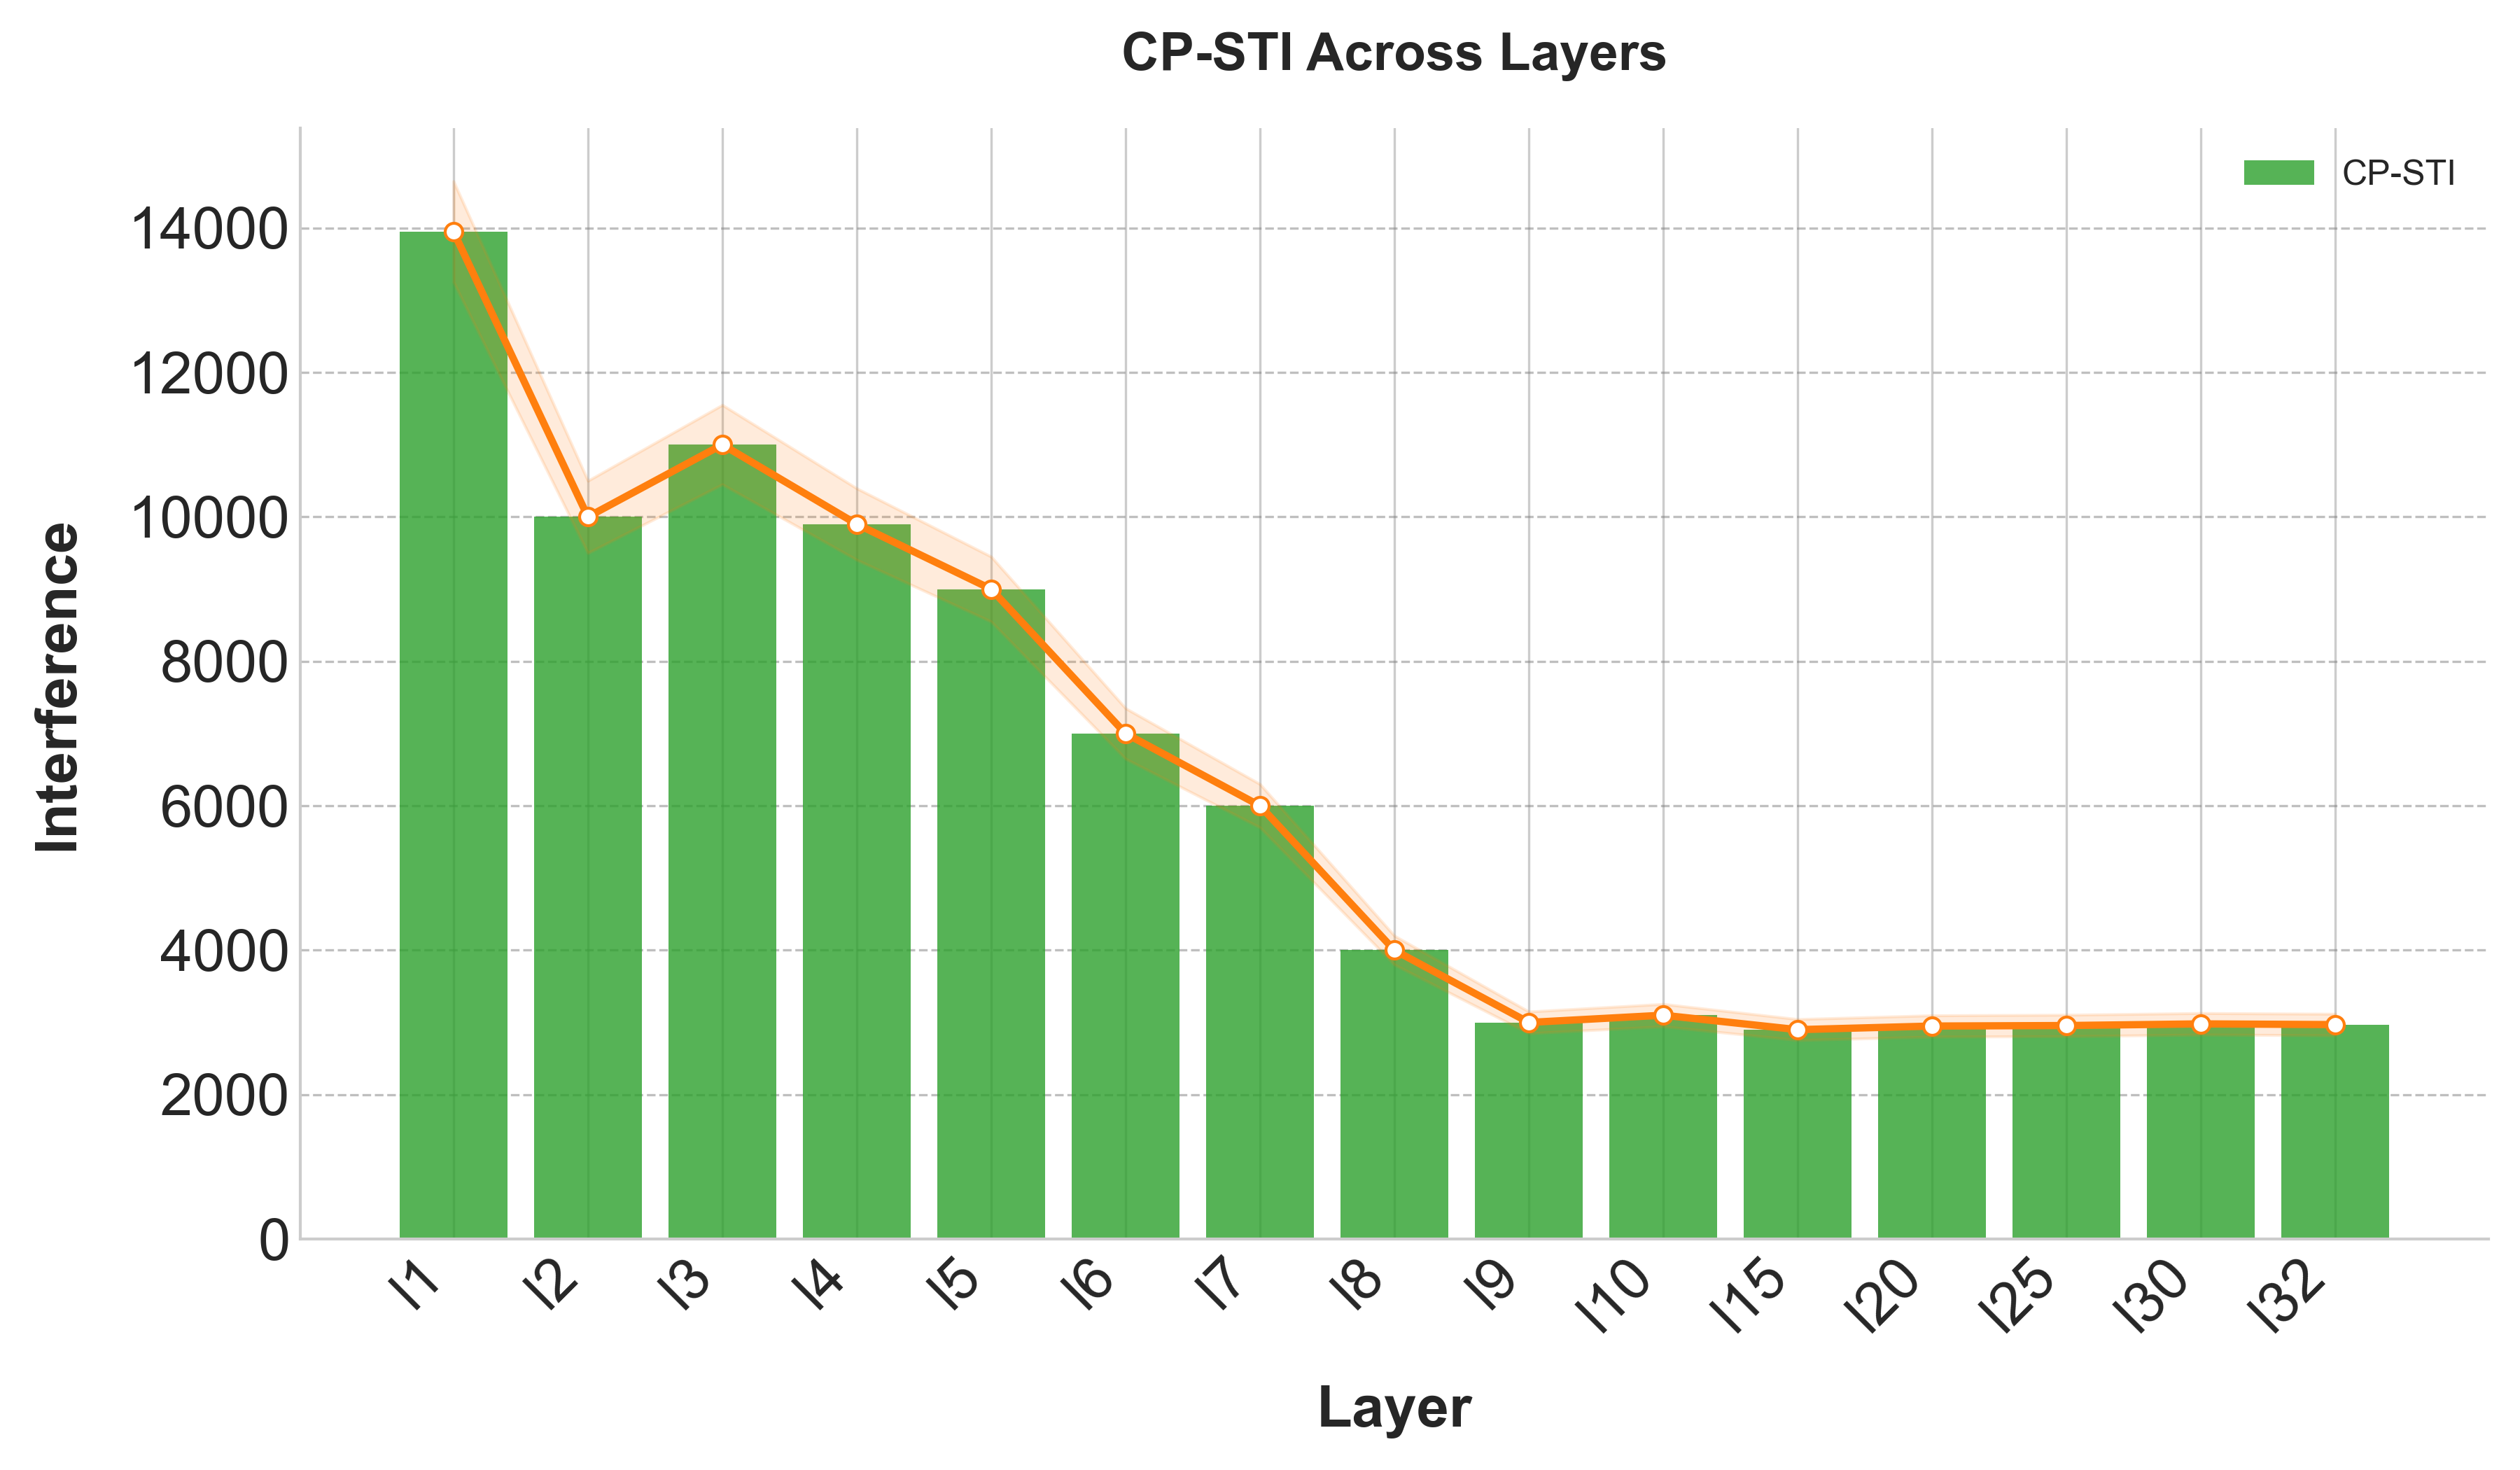
\includegraphics[width=\textwidth]{fig/cp_sti_across_layers.png}
%         \subcaption{CP-STI across 10 layers in the LLama 7B for Math and Code LoRA.}
%         \end{subfigure}
%         \hfill
%         \begin{subfigure}
%             {0.45\textwidth}
%             \centering
%             \includegraphics[width=\textwidth]{
%                 iclr2026/fig/rouge_l_heatmap_with_bolder_lines.png
%             }
%             \subcaption{Best performance for different alpha values. }
%         \end{subfigure}
%         % \caption{The number of clusters and accuracy (ACC) using Phi-3 3B (left)
%         % and Mistral 7B (right).}
%         \label{fig:cluster_performance}
%     \end{figure}





\begin{table}[t]
\centering
\small
\begin{tabular}{p{4cm} p{4.8cm} p{1.8cm} p{4.4cm}}
\toprule
Metric & Statistic & Value & Interpretation \\ 
\midrule
STI & Pearson(layer index, STI) & 0.755 & Positive linear trend across depth \\ 
STI & Spearman(layer index, STI) & 0.807 & Positive monotonic trend across depth \\ 
STI & mean(qkv\_proj)/mean(o\_proj) & 1.14x & Moderate projection asymmetry \\ 
\midrule
CP-STI & Pearson(layer index, log CP-STI) & -0.006 & Near-zero depth trend \\ 
CP-STI  & Spearman(layer index, log CP-STI) & -0.063 & Near-zero monotonic depth trend \\ 
CP-STI & mean(qkv\_proj)/mean(o\_proj) & 14.29x & Strong projection/magnitude asymmetry \\ 
CP-STI column-normalized & Pearson(layer, norm) & 0.306 & STI-comparable scale \\
CP-STI column-normalized & Spearman(layer, norm) & 0.324 & Moderate depth trend
\\
CP-STI off-diagonal & Pearson(layer, offdiag) & 0.420 \\
CP-STI off-diagonal & Spearman(layer, offdiag) & 0.533 \\
Diagonal dominance & mean diag fraction & 1.000 & \\









\bottomrule
\end{tabular}
\caption{Layer-wise interference statistics computed from per-layer TSV-STI and CP-STI. For depth correlation, layer-level scores are obtained by averaging o\_proj and qkv\_proj per layer. For CP-STI, log10 is used before correlation due to multi-order magnitude spread.}
\label{tab:interference_rebuttal}
\end{table}

As shown in the Figure \ref{fig:sti}, we visualize the STI metric across layers with five tasks based on Phi-3. We can notice that STI shows a clear depth thread. Aggregating over o-proj and qkv-proj, STI increases with layer depth (Pearson with layer index $\approx$ 0.755, Spearman $\approx$ 0.807), indicating stronger interference in deeper layers for this run. This conclusion does not match the conclusion int the TSV paper, where the interference is in the lower layer instead of higher layers. In addition, in STI, qkv-proj is consistently higher than o-proj (mean ratio $\approx$=1.14x), and top-interference points are mostly qkv-proj in deeper layers. (17, 19,22-24). As shown in Table \ref{tab:interference_rebuttal}, CP-STI is much larger on qkv-proj than o-proj (mean ratio=14.3x), showing strong layer/projection heterogeneity. Off-diagonal CP-STI has 0.53, and normalized CP-STI has 0.32, indicating the same direction of trend (deeper layers show stronger interference signals.

\begin{figure}
    \centering
    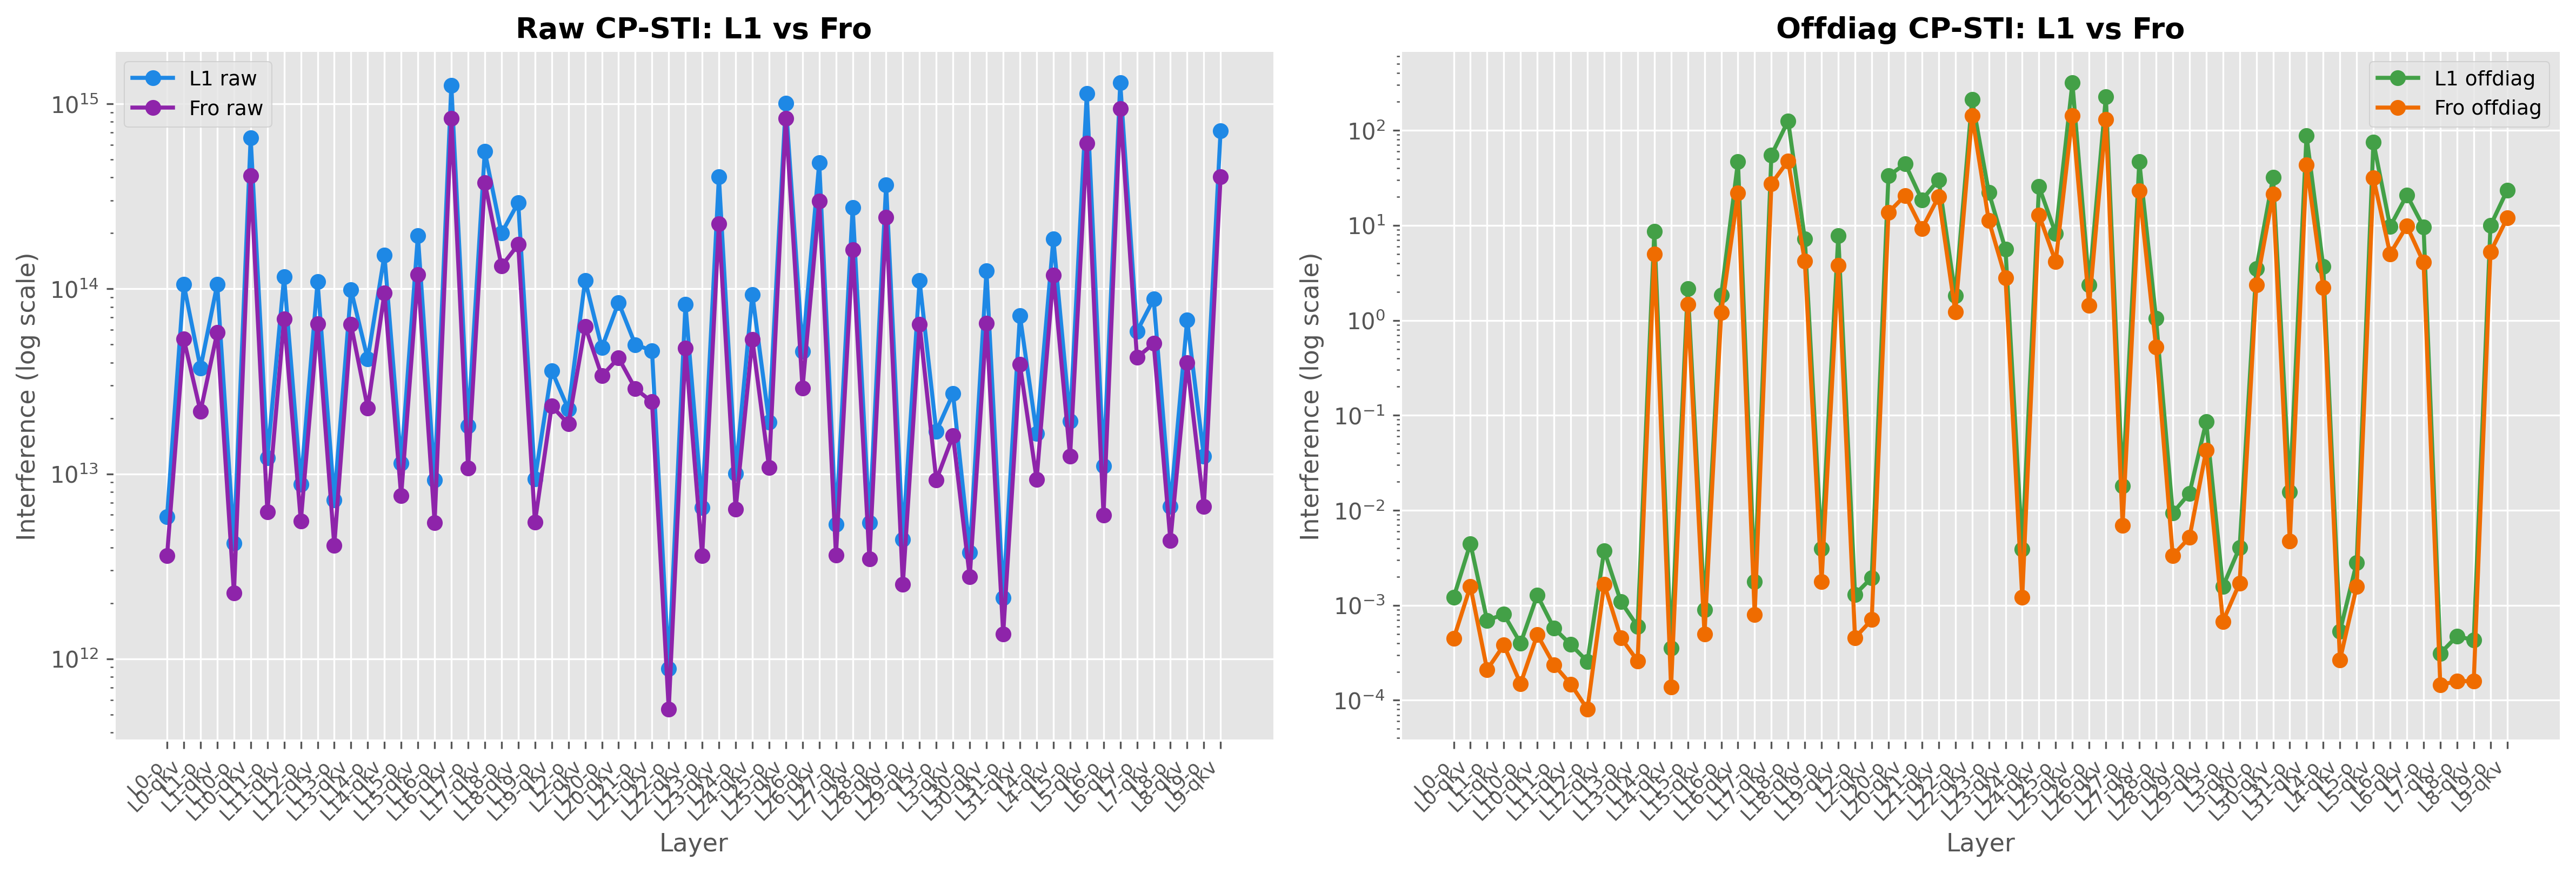
\includegraphics[width=\linewidth]{fig/cpmergeafter_cp_sti_l1_vs_fro_across_layers_beautified.png}
    \caption{left: raw CP-STI, right: off-diagonal CP-STI.}
    \label{fig:cp-sti-l1-f}
\end{figure}

We also compared CP-STI computed with L1 and Frobenius norms in Figure \ref{fig:cp-sti-l1-f}. The key observation is that both norms produce highly consistent layer-wise patterns: peaks and valleys occur at the same layers in both panels. Frobenius values are typically lower in magnitude, but the relative ranking across layers is preserved, indicating that the interference signal is not an artifact of a specific norm.
Importantly, this consistency also holds for the off-diagonal variant: L1-offdiag and Fro-offdiag track each other closely across layers. Therefore, the metric’s conclusion (where interference is stronger/weaker across layers) is norm-robust.



% We study the task interference on each layer according to Eq. (\ref{eq:cp_sti}). As shown in the Fig. \ref{fig:cp_str_interference}, the interference is higher in the lower layer and decreases in the deeper layers. This may indicate that the lower layers capture common features and deeper layers are more specialized for specific tasks. 

\subsection{Rank $R$ of the CP decomposition.}
\label{sec:rank_analyse}

        \begin{wrapfigure}[15]
        {r}{0.4\textwidth}
        \vspace{-5pt}
        \small
        \centering
        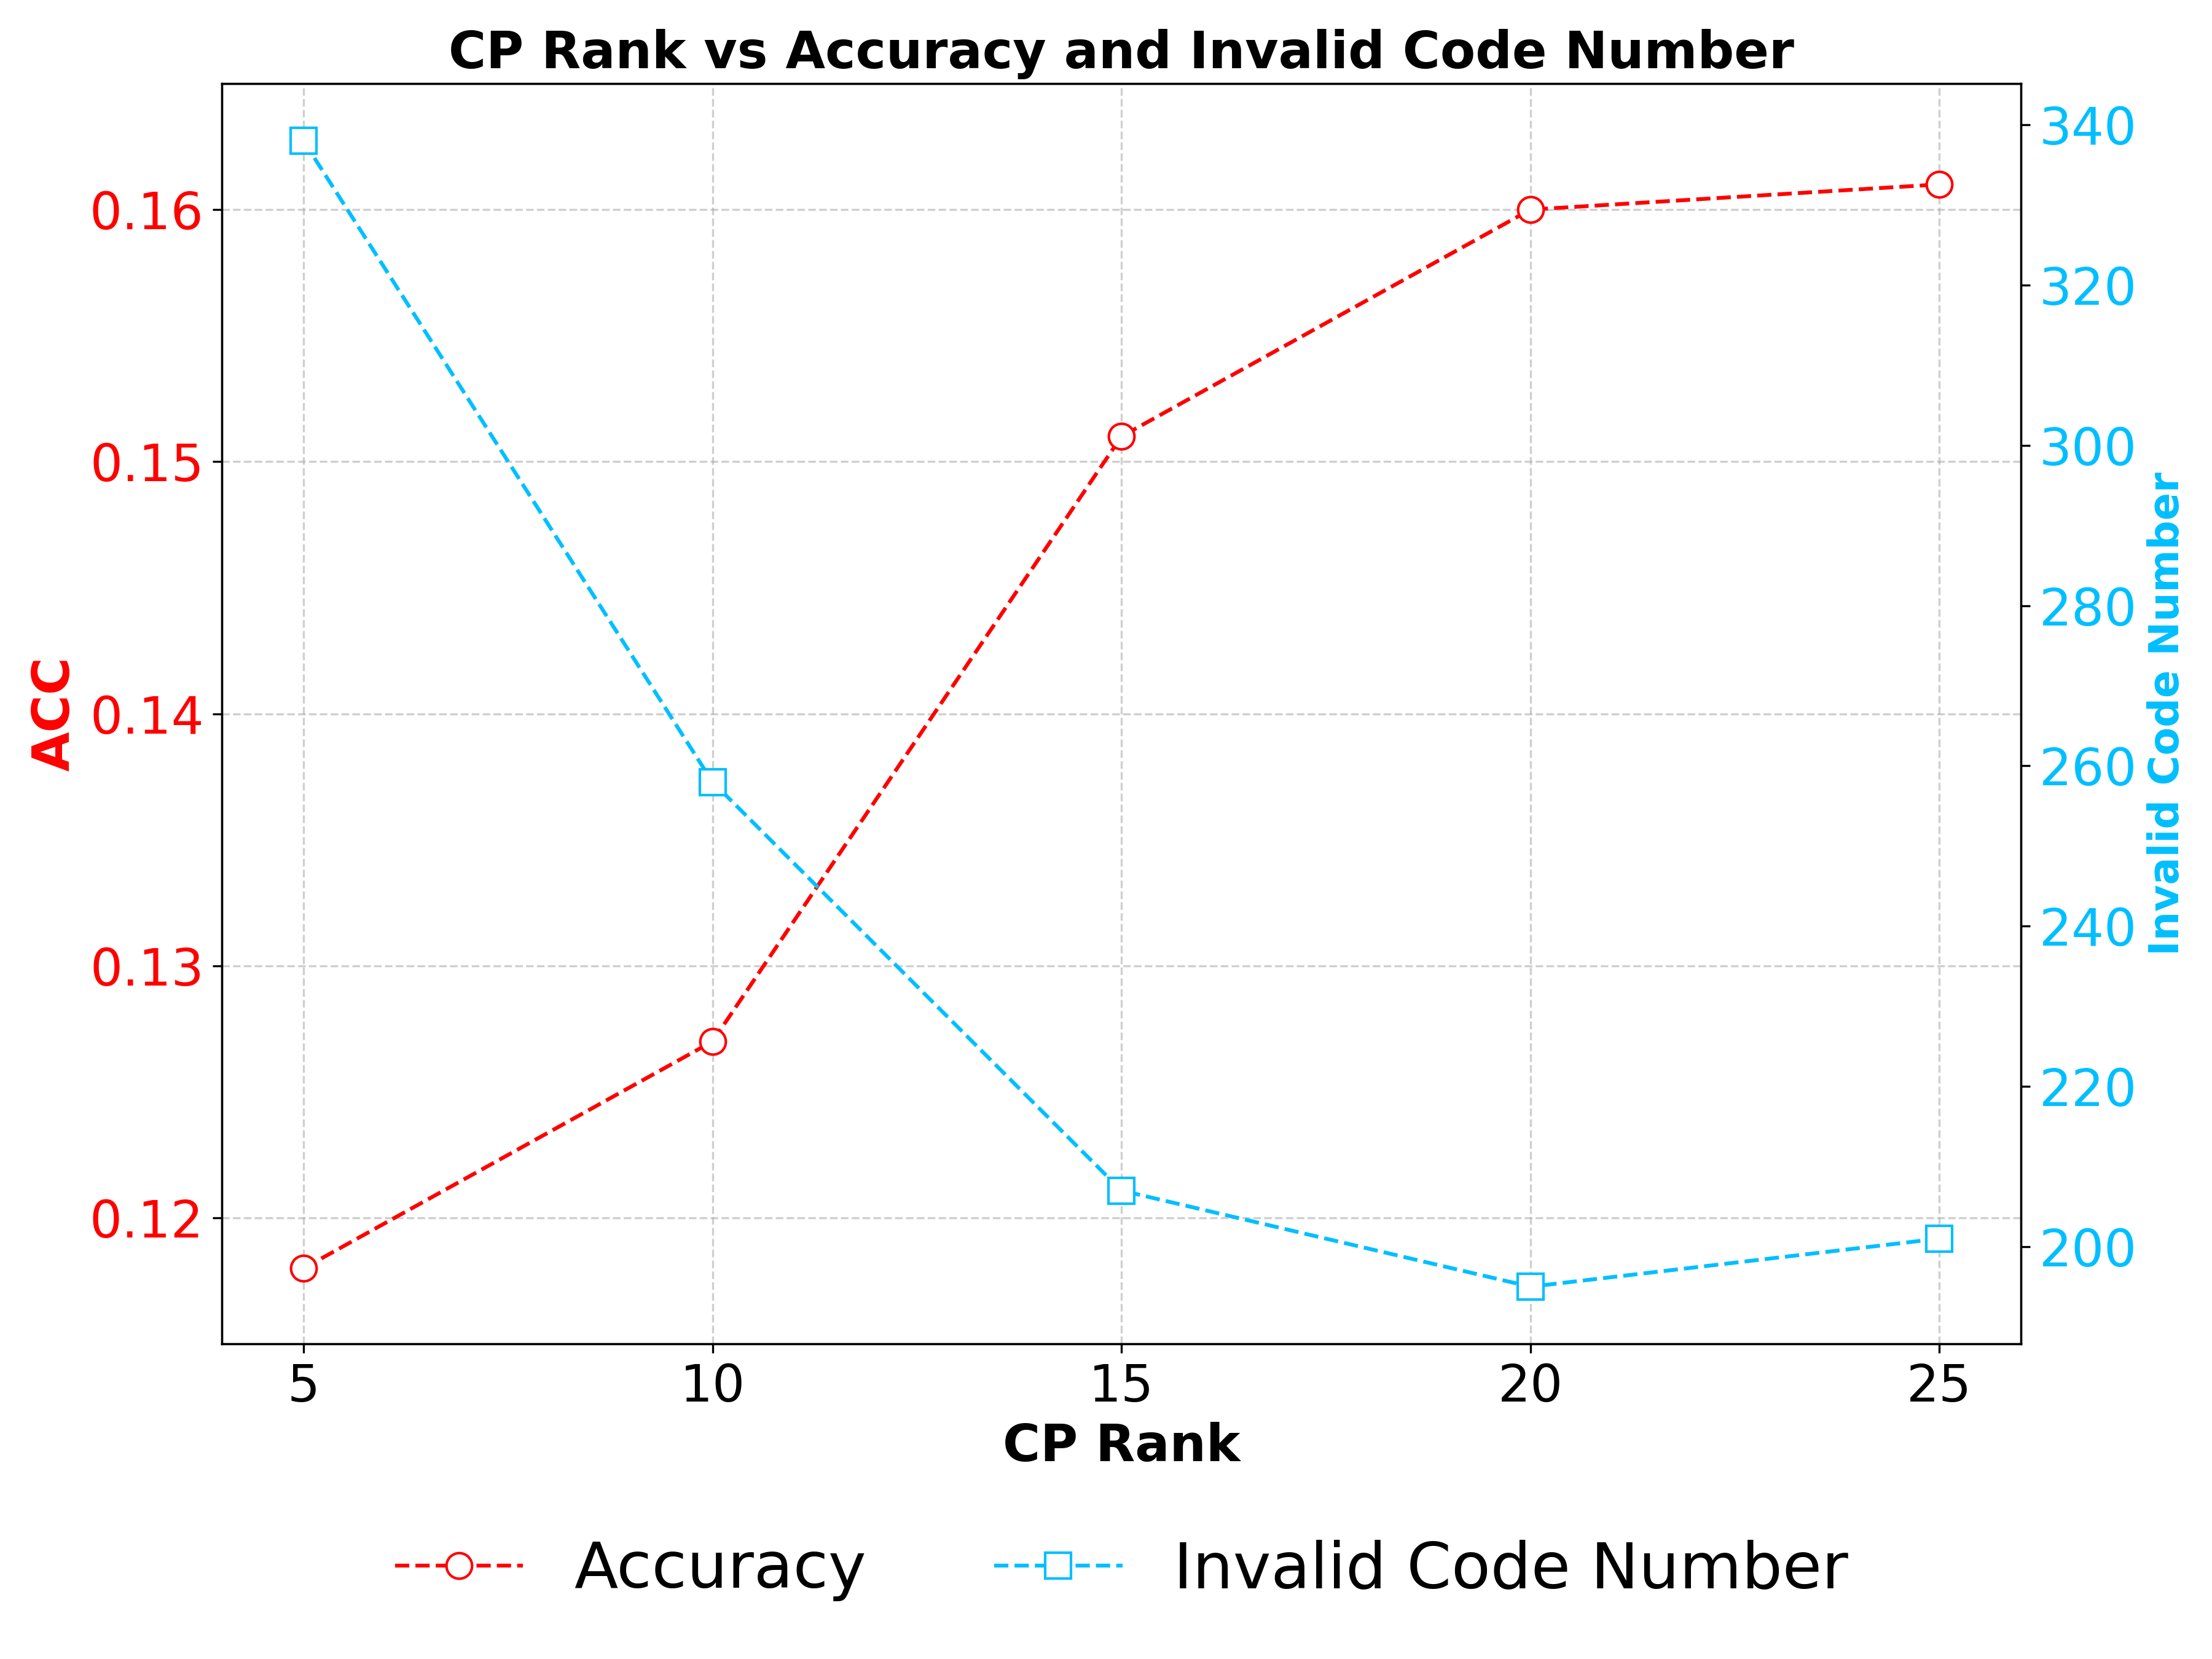
\includegraphics[width=0.40\textwidth]{fig/CP_rank_vs_ACC.png}
        \caption{The impact of CP rank on model performance and generation quality for the GSM-8K-hard benchmark.}
        \label{fig:CP_rank_performance}
    \end{wrapfigure}

    CP decomposition factorizes a tensor into a sum of $R$ rank‑one components. \citet{wang2023parameter}
    observed that increasing $R$ can improve performance on cross‑modal tasks. We
    investigate how the CP rank affects our method’s performance on the GSM8K‑hard
    dataset (Fig.\ref{fig:CP_rank_performance}). The left plot (“CP Rank vs.
    Accuracy”) shows accuracy rising from ~0.12 at rank 5 to a peak of ~0.15 at rank
    20, with no further gains beyond rank 25. This suggests that higher ranks
    capture richer patterns, but benefits plateau after rank 20. The right plot (“CP
    Rank vs. Invalid Code”) shows invalid code outputs dropping from ~340 at rank
    5 to ~200 at rank 20, with little improvement at higher ranks. Overall, increasing
    the CP rank improves both accuracy and output validity up to an optimal point
    (around rank 20), after which returns diminish, highlighting the importance
    of selecting an appropriate rank to balance performance and efficiency in
    mitigating task interference in skill composition tasks.

    % \begin{figure}[h]
    %     \centering
    %     \begin{subfigure}
    %         {0.45\textwidth}
    %         \centering
    %         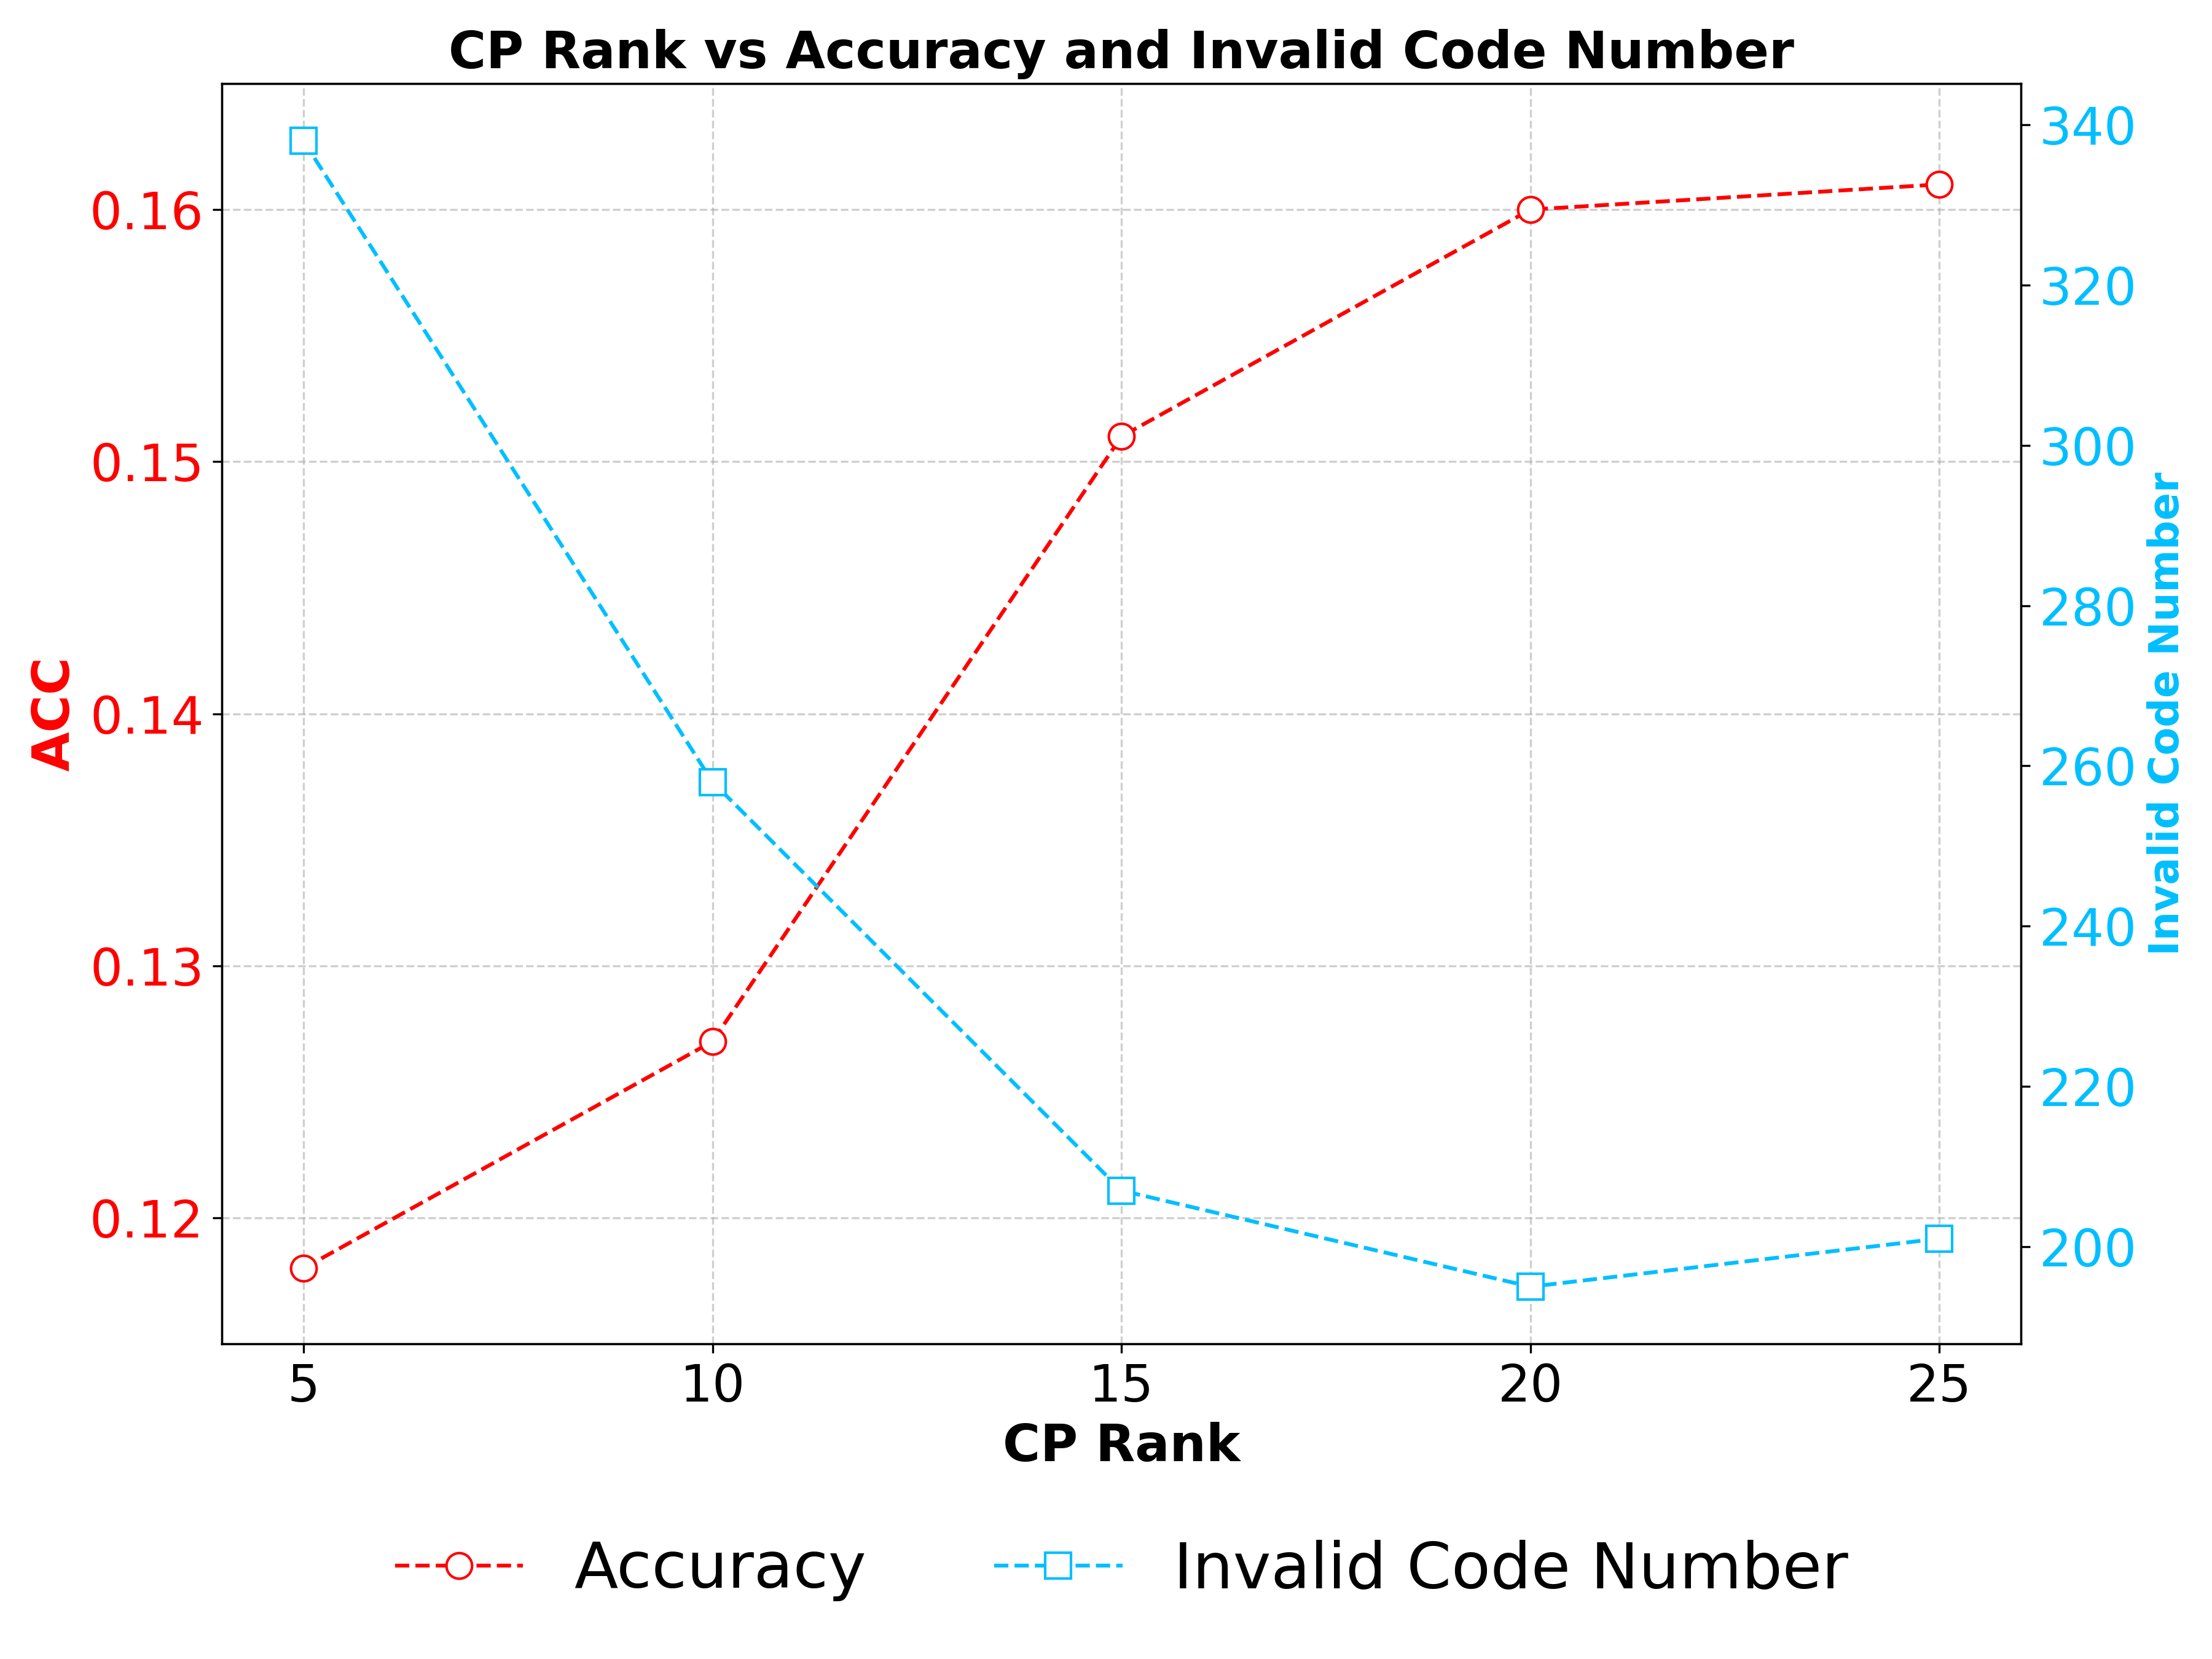
\includegraphics[width=\textwidth]{fig/CP_rank_vs_ACC.png}
    %     \end{subfigure}
    %     \hfill
    %     \begin{subfigure}
    %         {0.45\textwidth}
    %         \centering
    %         \includegraphics[width=\textwidth]{fig/CP_rank_vs_invalid_code.png}
    %     \end{subfigure}
    %     \caption{The impact of CP rank on model performance and generation
    %     quality for the GSM-8K benchmark.}
    %     \label{fig:CP_rank_performance}
    % \end{figure}


\subsection{Alpha analysis}

\begin{wrapfigure}[13]{r}
{0.4\textwidth}
\vspace{-15pt}
\centering
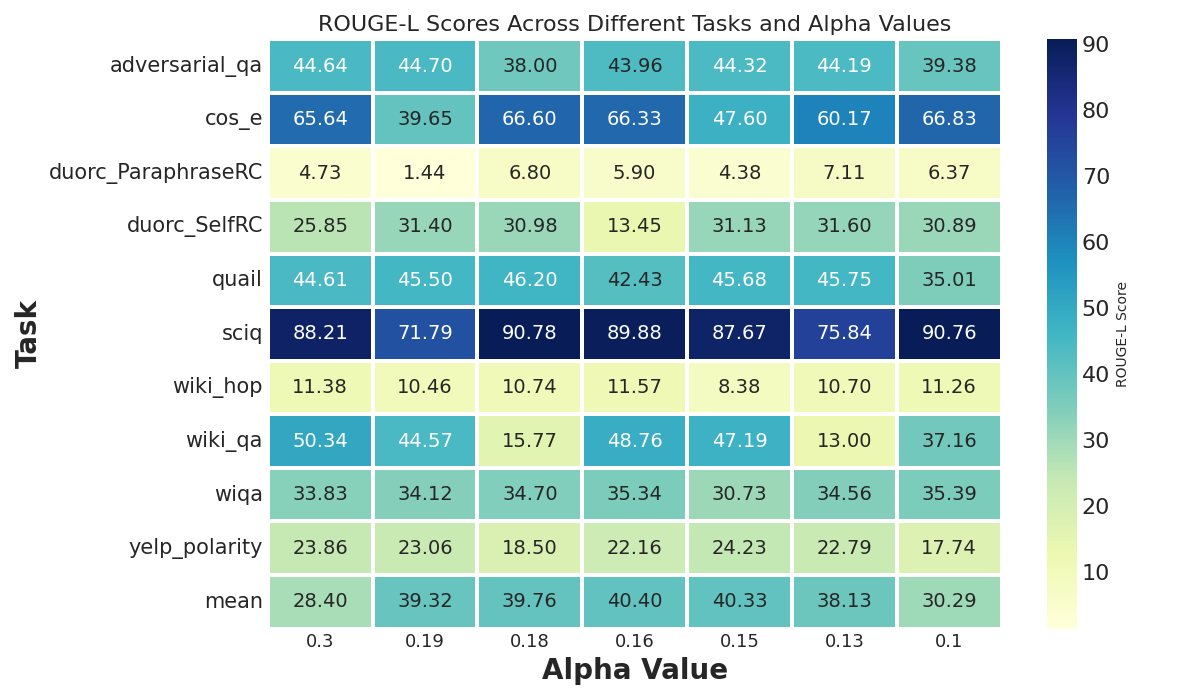
\includegraphics[width=0.45\textwidth]{fig/rouge_l_heatmap_with_bolder_lines.png}
\caption{Best performance for different alpha values over 10 held-in Flan datasets. }
\label{fig:alpha}
\end{wrapfigure}

The alpha parameter effectively scales the influence of the adapter's output before it is added back to the weights of the original model. Table~\ref{fig:alpha} reports the ROUGE-L scores for 10 held-in Flan tasks across seven $\alpha$ values ranging from 0.3 to 0.1. The results highlight the critical importance of the $\alpha$ hyperparameter for LoRA merging methods—including CP merging, \texttt{knots}, TSV merging, and ISO merging. Notably, the optimal $\alpha$ is not universal but depends on the specific task, underscoring the need for careful tuning. On average, moderate values (e.g., $\alpha=0.15$–$0.18$) yield the best performance. For all experiments, $\alpha$ was selected based on performance over a validation set of 1,000 examples. Finally, we use 0.25 for TSV merging and 0.50 for Knots. 

\subsection{Computation Cost}



CP merging conducts the tensor decomposition, while the SVD-based merging conducts the matrix decomposition. In this subsection, we study the computation cost compared to these methods. We compare the computation cost for [3, 5, 10] LoRA adapters. The computation is based on the Phi-3B on Flan datasets. We run experiments using one A100 GPU card. As depicted in Tab.\ref{tab:computation_copmarison}, TSV merging and Knots exhibit substantial growth in cost as the number of LoRA modules increases, reaching up to 1320–1980 seconds with 10 LoRAs. In contrast, CP merging is significantly more efficient, requiring only 31–58 seconds across all settings—an order-of-magnitude improvement over the other baselines.
\begin{table}
    \centering
    \begin{tabular}{l|ccc}
    \toprule
      Model  & 3 LoRA & 5 LoRA & 10 LoRA \\
    \midrule
     TSV merging & 350s & 553s & 1320s\\
     Knots & 540s & 780s & 1980s\\
     \midrule
     CP merging & \textbf{31s} & \textbf{38s} & \textbf{58s}\\
     \bottomrule
    \end{tabular}
    \caption{Computation cost (seconds) compared with various LoRA merging approaches. We use Phi-3B as a backbone model. }
    \label{tab:computation_copmarison}
\end{table}

\section{Discussion}

The current formulation of CP merge assumes a static set of $N$ adapters merged into a third-order tensor $\mathcal{T} \in \mathbb{R}^{N \times d \times d}$. However, in dynamic "Open World" environments, new task-specific adapters are frequently released post-initial merging. A potential concern is the computational overhead of re-performing the full CP decomposition as the task dimension $N$ grows.

To address this, our framework can be extended to an incremental update strategy. Since the row-mode factor $B$ and column-mode factor $C$ capture the fundamental geometric structures of the weight space across layers, these can be treated as a fixed basis once the initial model is established. For a newly arriving adapter $\Delta_{N+1}$, instead of re-decomposing the entire tensor, we can solve a linear sub-problem to find a new task-mode vector $a_{N+1}$ that minimizes the reconstruction error:

\begin{equation}
    \min_{a_{N+1}} \|\Delta_{N+1} - \sum_{r=1}^{R} a_{N+1,r} (b_r \circ c_r)\|_F
\end{equation}

In this context, $a_{N+1}$ serves as the task coefficient, effectively embedding the new task into the pre-existing shared knowledge space without altering the established parameters of prior models. This approach significantly reduces the computational complexity from full tensor factorization to a simple least-squares projection, ensuring the engineering viability of our method in evolving multi-task systems.


\section{Conclusion}
We propose a novel LoRA merging method using Canonical Polyadic (CP) decomposition. Unlike existing SVD-based methods that decompose each LoRA adapter with matrix decomposition, CP merging factorizes multiple adapters in a unified manner. This allows us to disentangle task-specific components from those that are shared across tasks. Our comprehensive experiments show that CP merging consistently outperforms strong SVD-based baselines across various benchmarks, including in-domain multi-tasks, zero-shot tasks, and skill composition tasks. These results confirm that our method effectively preserves essential task knowledge while significantly reducing cross-task interference. This unified factorization approach is a key advantage over conventional merging techniques. Our findings offer a new perspective on how knowledge is represented and merged within LoRA adapters. 



\subsubsection*{Acknowledgments}
Use unnumbered third level headings for the acknowledgments. All
acknowledgments, including those to funding agencies, go at the end of the paper.
Only add this information once your submission is accepted and deanonymized. 

\bibliography{tmlr}
\bibliographystyle{tmlr}

\newpage
\appendix
\section{Appendix}

\subsection{Limitations}

In this work, we evaluate our approach on natural language tasks using models such as Phi-3B, Mistral-7B, and LLaMA-7B. Extending the analysis to larger-scale models remains an important direction for future research. Our experiments show that CP merging achieves superior performance compared to SVD-based LoRA merging methods. However, on held-out and zero-shot tasks, uniform merging achieves competitive—and in some cases even better—results, suggesting that improving the generalization ability of LoRA merging methods remains an open challenge. Moreover, our current evaluation is limited to at most 10 tasks. Scaling to a larger number of tasks presents additional challenges for LoRA merging, which we plan to investigate in future work.

\paragraph{Use of large language models statement}

We use the LLM to polish the writing. All other parts, including experimental results, analyses 
were written by the authors and carefully verified for accuracy before and after any LLM-assisted
editing.




\subsection{Skill Composition Tasks}
\label{sec:skill_composition}

\begin{figure}[h]
        \centering
        \begin{prompt}
            [title={GSM8k vs GSM8k-hard}] { \textcolor{blue}{GSM8k}: A robe takes \textcolor{red}{2} bolts of blue fiber and half that much white fiber. How many bolts in total does it take?

            Reference Answer: 18

            \textcolor{blue}{GSM8k-hard}: A robe takes \textcolor{red}{2287720} bolts of blue fiber and half that much white fiber. How many bolts in total does it take?

            Reference Answer: 3,431,580 }
        \end{prompt}
        \caption{The comparison between GSM8k and GSM8k-hard. The GSM8K uses a larger
        number to replace the original number.}
        \label{prompt-verifier}
\end{figure}

    \cite{prabhakar2024lora} have used LoRA merging to achieve the \textit{skill
    composition}. Skill here refers to specific capabilities that the LLM needs for
    customization to downstream use cases. For example, achieving a high score in
    GSM8k benchmark \cite{cobbe2021training} needs good \textit{commonsense} and
    \textit{arithmetic} skills.


    To explicitly examine how reducing task interference, we evaluate CP merging on hard math word problems.
    Compared to GSM‑8K \citep{cobbe2021training}, GSM8K‑hard \citep{gao2023pal} contains
    problems of similar types but with more complex arithmetic operations.
    \citet{gao2023pal} propose a program‑aided method in which an LLM first generates
    a program as an intermediate reasoning step and then executes it using a Python
    interpreter to obtain the final answer. This setting requires the LLM to be
    proficient in both mathematical reasoning (to analyze the problem) and
    coding (to translate the reasoning into executable code). Following the same experimental setting in  \citet{prabhakar2024lora},
    we train separate LoRA adapters for math and code skills.

    \subsubsection{GSM8k-hard Results}
    \begin{table}[h]
        \centering
        \begin{tabular}{l|cc}
            \toprule Model               & ACC             & Invalid Code\\
            \midrule \textbf{BASE}       & 0.0430          & 524          \\
            \textbf{LoRA(math)}          & 0.1175          & 562          \\
            \textbf{LoRA(code)}          & 0.0796          & 159          \\
            \textbf{Multi-task}          & 0.1349          & 413          \\
            \textbf{Uniform}             & 0.1296          & 217          \\
            \textbf{Ties-merging}        & 0.1060          & 223          \\
            \textbf{Task Arithmetic}     & 0.1190          & 232          \\
            \textbf{Ties w/DARE}         & 0.1162          & 227          \\
            \textbf{TA w/DARE}           & 0.1200          & 247          \\
            \textbf{ISO Merging} & 0.0840 & 394 \\
            \textbf{TSV Merging}         & 0.1349          & 224          \\
            
            \textbf{Knots} & 0.1344 & 263\\
            \midrule \textbf{CP merging} & \textbf{0.1569} & 201          \\
            \midrule
            \bottomrule
        \end{tabular}
        \caption{Evaluation results on MATH-hard tasks. "Invalid" is the number of
        invalid codes that can not be executed by Python.}
        \label{tab:math-hard}
    \end{table}
    As depicted in Tab. \ref{tab:math-hard}, we evaluate the accuracy scores on
    the GSM-8k hard benchmark across various models. The base model achieves a modest
    accuracy of 0.043, highlighting its limitations in tackling GSM-hard tasks
    effectively. By training a LoRA adapter with the MathQA instruction dataset,
    we enhance the model's mathematical capabilities. Similarly, training with
    the Alpaca-code dataset boosts the model's coding proficiency. Combining both
    MathQA and Alpaca-code datasets in a single adapter yields an accuracy of 0.1349.
    Merging the math and coding skills through LoRA merging results in an
    accuracy of 0.1296, demonstrating the potential to integrate these abilities. TSV Merging and Knots perform similarly in terms of accuracy, with scores of 0.1349 and 0.1344, respectively. However, TSV Merging generates fewer invalid codes (224) compared to Knots (263), suggesting it is slightly more stable in this regard.
    Among the competing baselines, our proposed CP merging achieves the highest accuracy
    of 0.1569. Additionally, we assess the "invalid code" metrics across methods.
    Notably, the LoRA code approach reduces invalid code instances from 524 in the
    base model to 159, indicating improved code quality. 

    The results demonstrate that our CP merging effectively reduces task
    interference by integrating math and coding skills, as evidenced by the lower
    number of invalid codes (201) compared to the base model (524) and other methods. In conclusion, CP merging not only achieves the highest accuracy but also maintains a low rate of invalid code generation, clearly demonstrating its superior performance in handling complex math-hard tasks.





\subsection{SVD illustration of U and V}

The similarities in the $U$ and $V$ matrices can reflect correlations among different experts. To empirically investigate whether SVD fails to capture inter-task interference, we compute the pairwise cosine similarity of the $U$ and $V$ matrices across five diverse task experts (Figure \ref{fig:SVD_visualization}). As observed in the heatmaps, the off-diagonal similarity scores are consistently low, suggesting that SVD factors are highly task-specific and lack a common orientation. Specifically, the $V$ matrix similarity (right) shows that the input-side features of different tasks are nearly orthogonal. This confirms that a naive merge of SVD-based adapters would result in information conflict, as the model would attempt to project different task logic onto misaligned subspaces.

% This observation provides the primary motivation for our CP-based approach, which overcomes this 'basis-mismatch' by factorizing all tasks simultaneously within a higher-order tensor framework, thereby ensuring a consistent and aligned parameter space.



\begin{figure}[h]
        \centering
        \begin{subfigure}
            \centering
            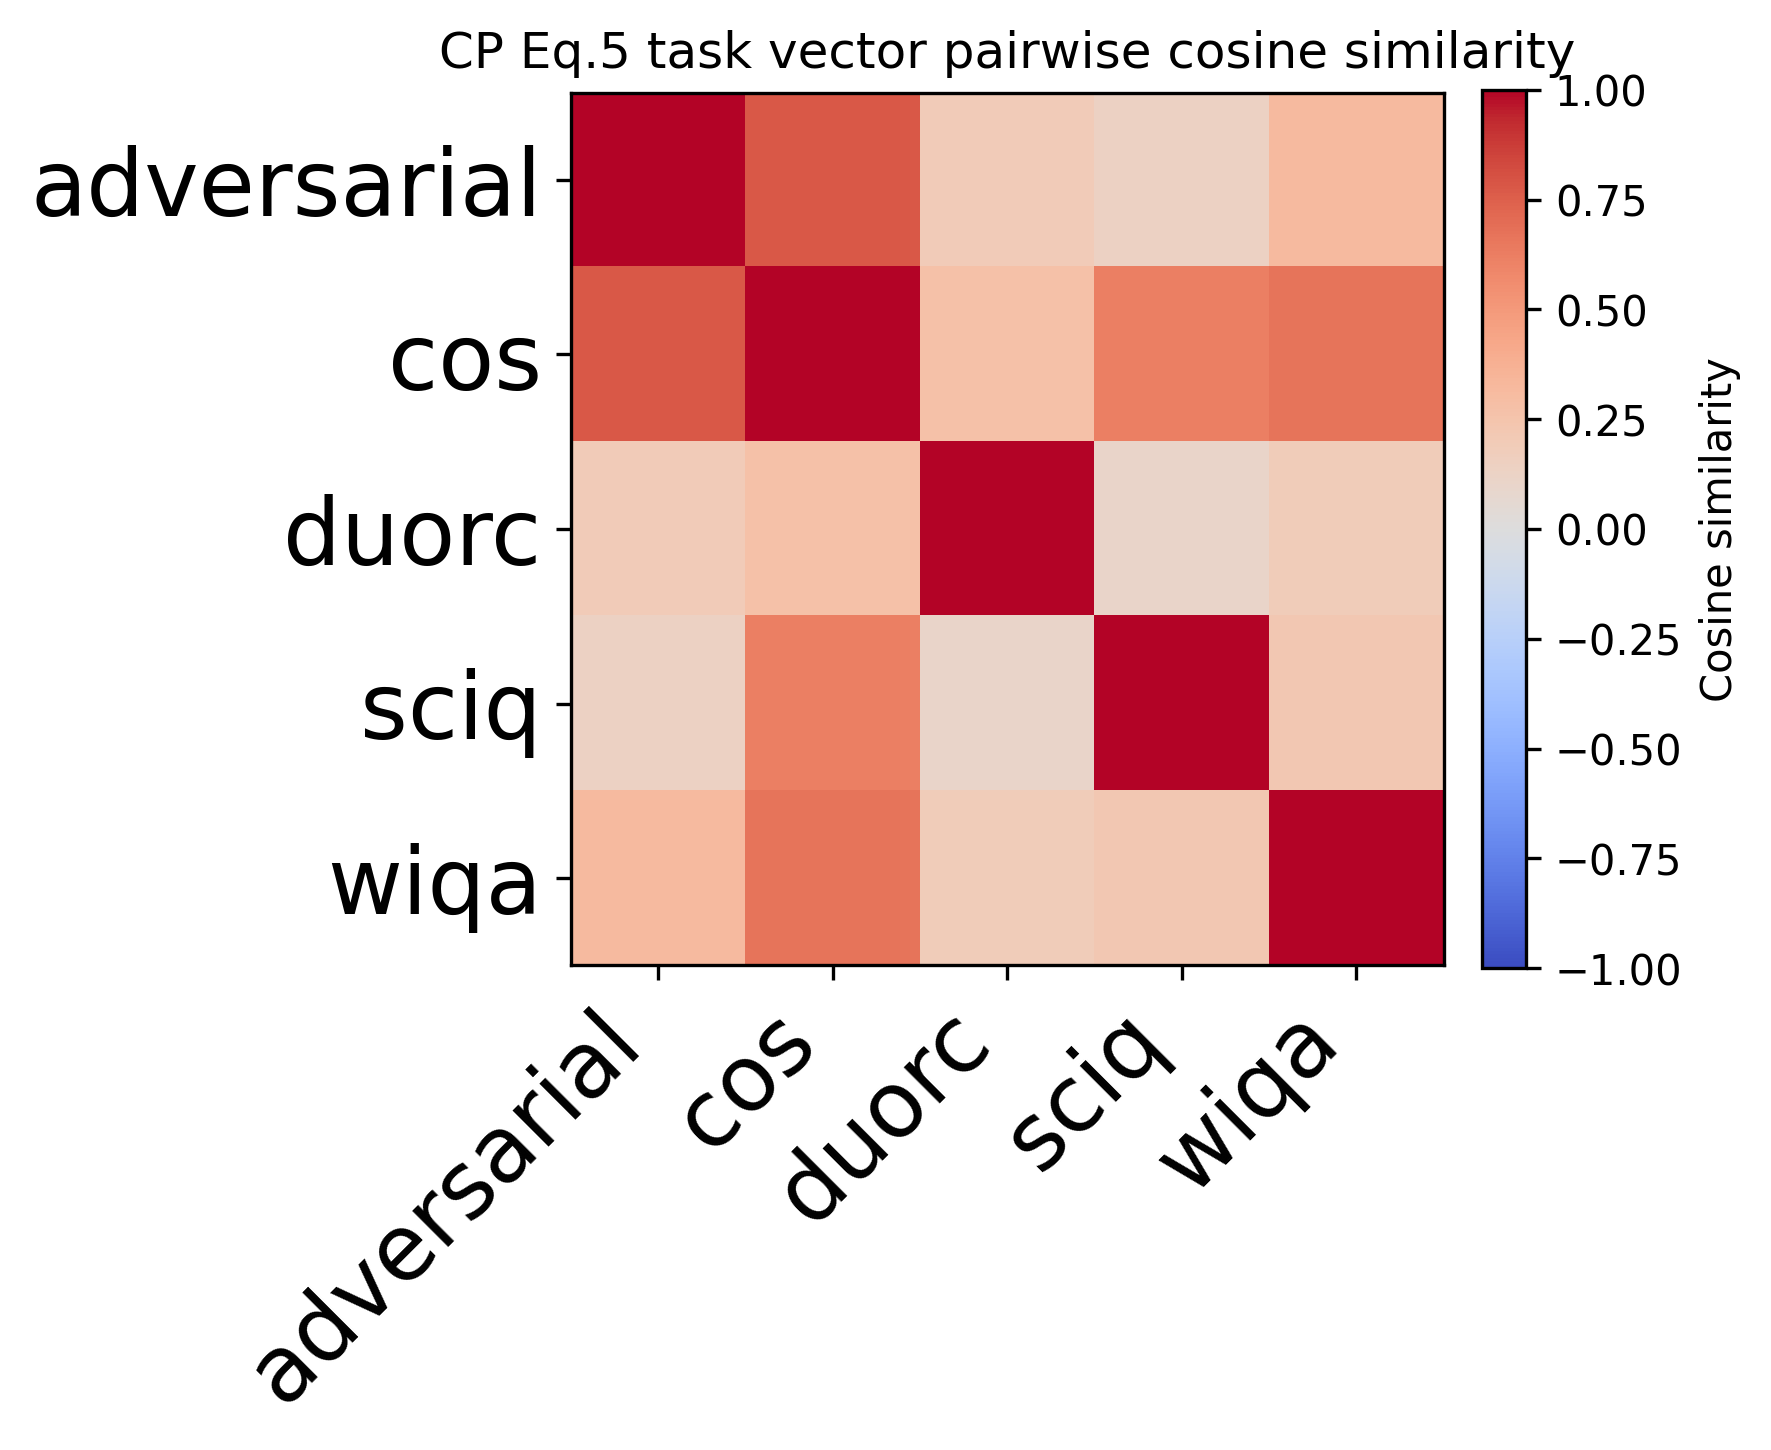
\includegraphics[width=0.28\textwidth]{fig/cpmergeafter_cp_eq5_task_matrix_cosine_similarity_model.layers.0.self_attn.o_proj.png}
        \end{subfigure}
        \hfill
        \begin{subfigure}
            \centering
            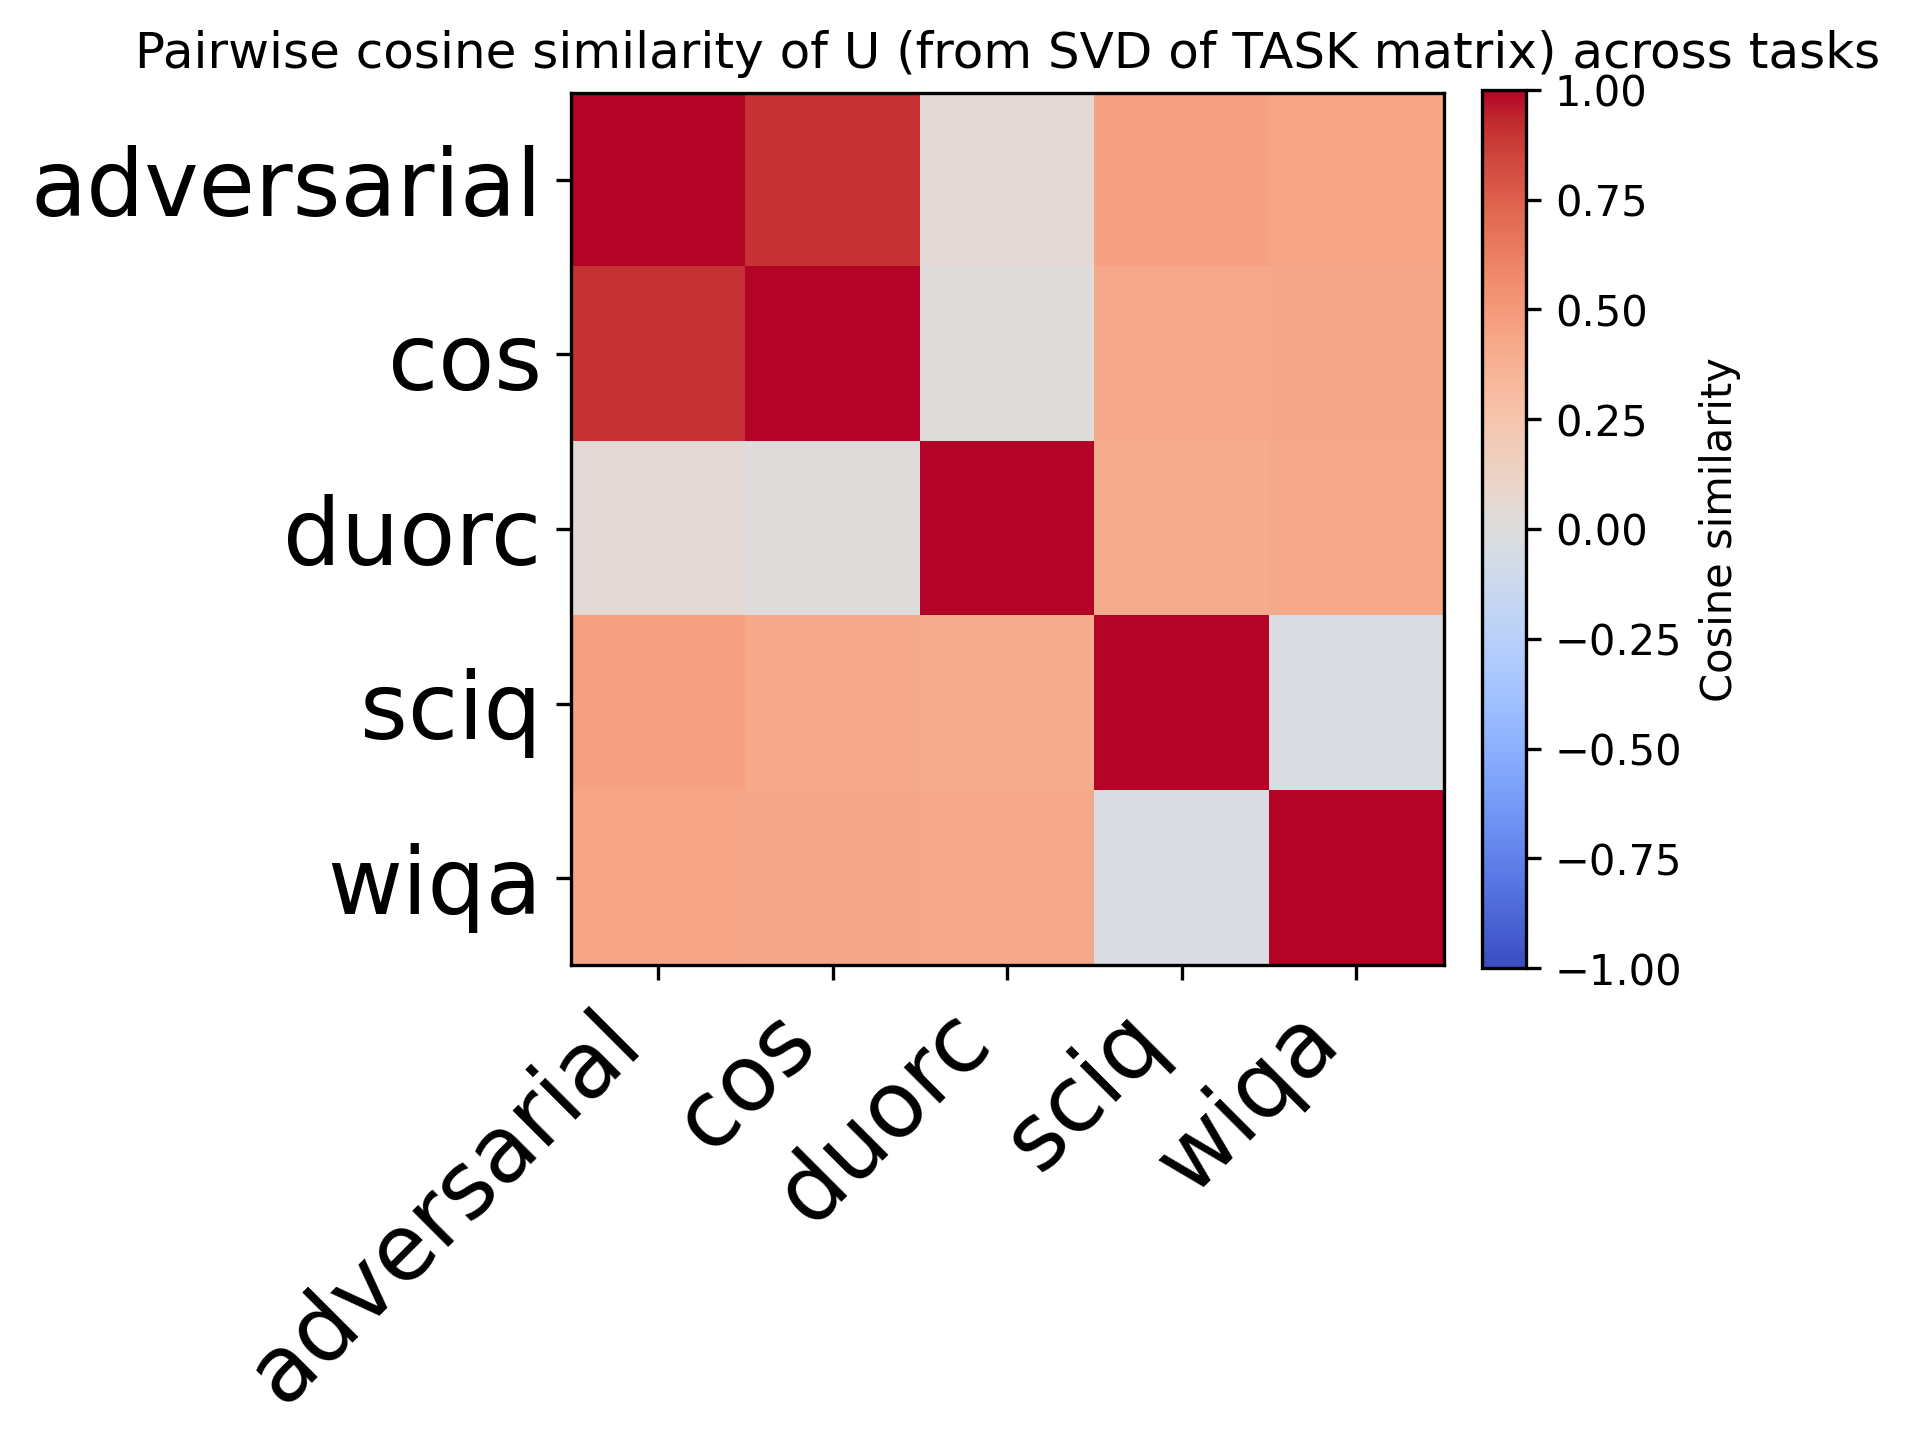
\includegraphics[width=0.30\textwidth]{fig/cpmergeafter_svd_u_cosine_similarity.png}
            % \subcaption{The number of clusters and accuracy (ACC) using Phi-3 3B}
        \end{subfigure}
        \hfill
        \begin{subfigure}
            \centering
            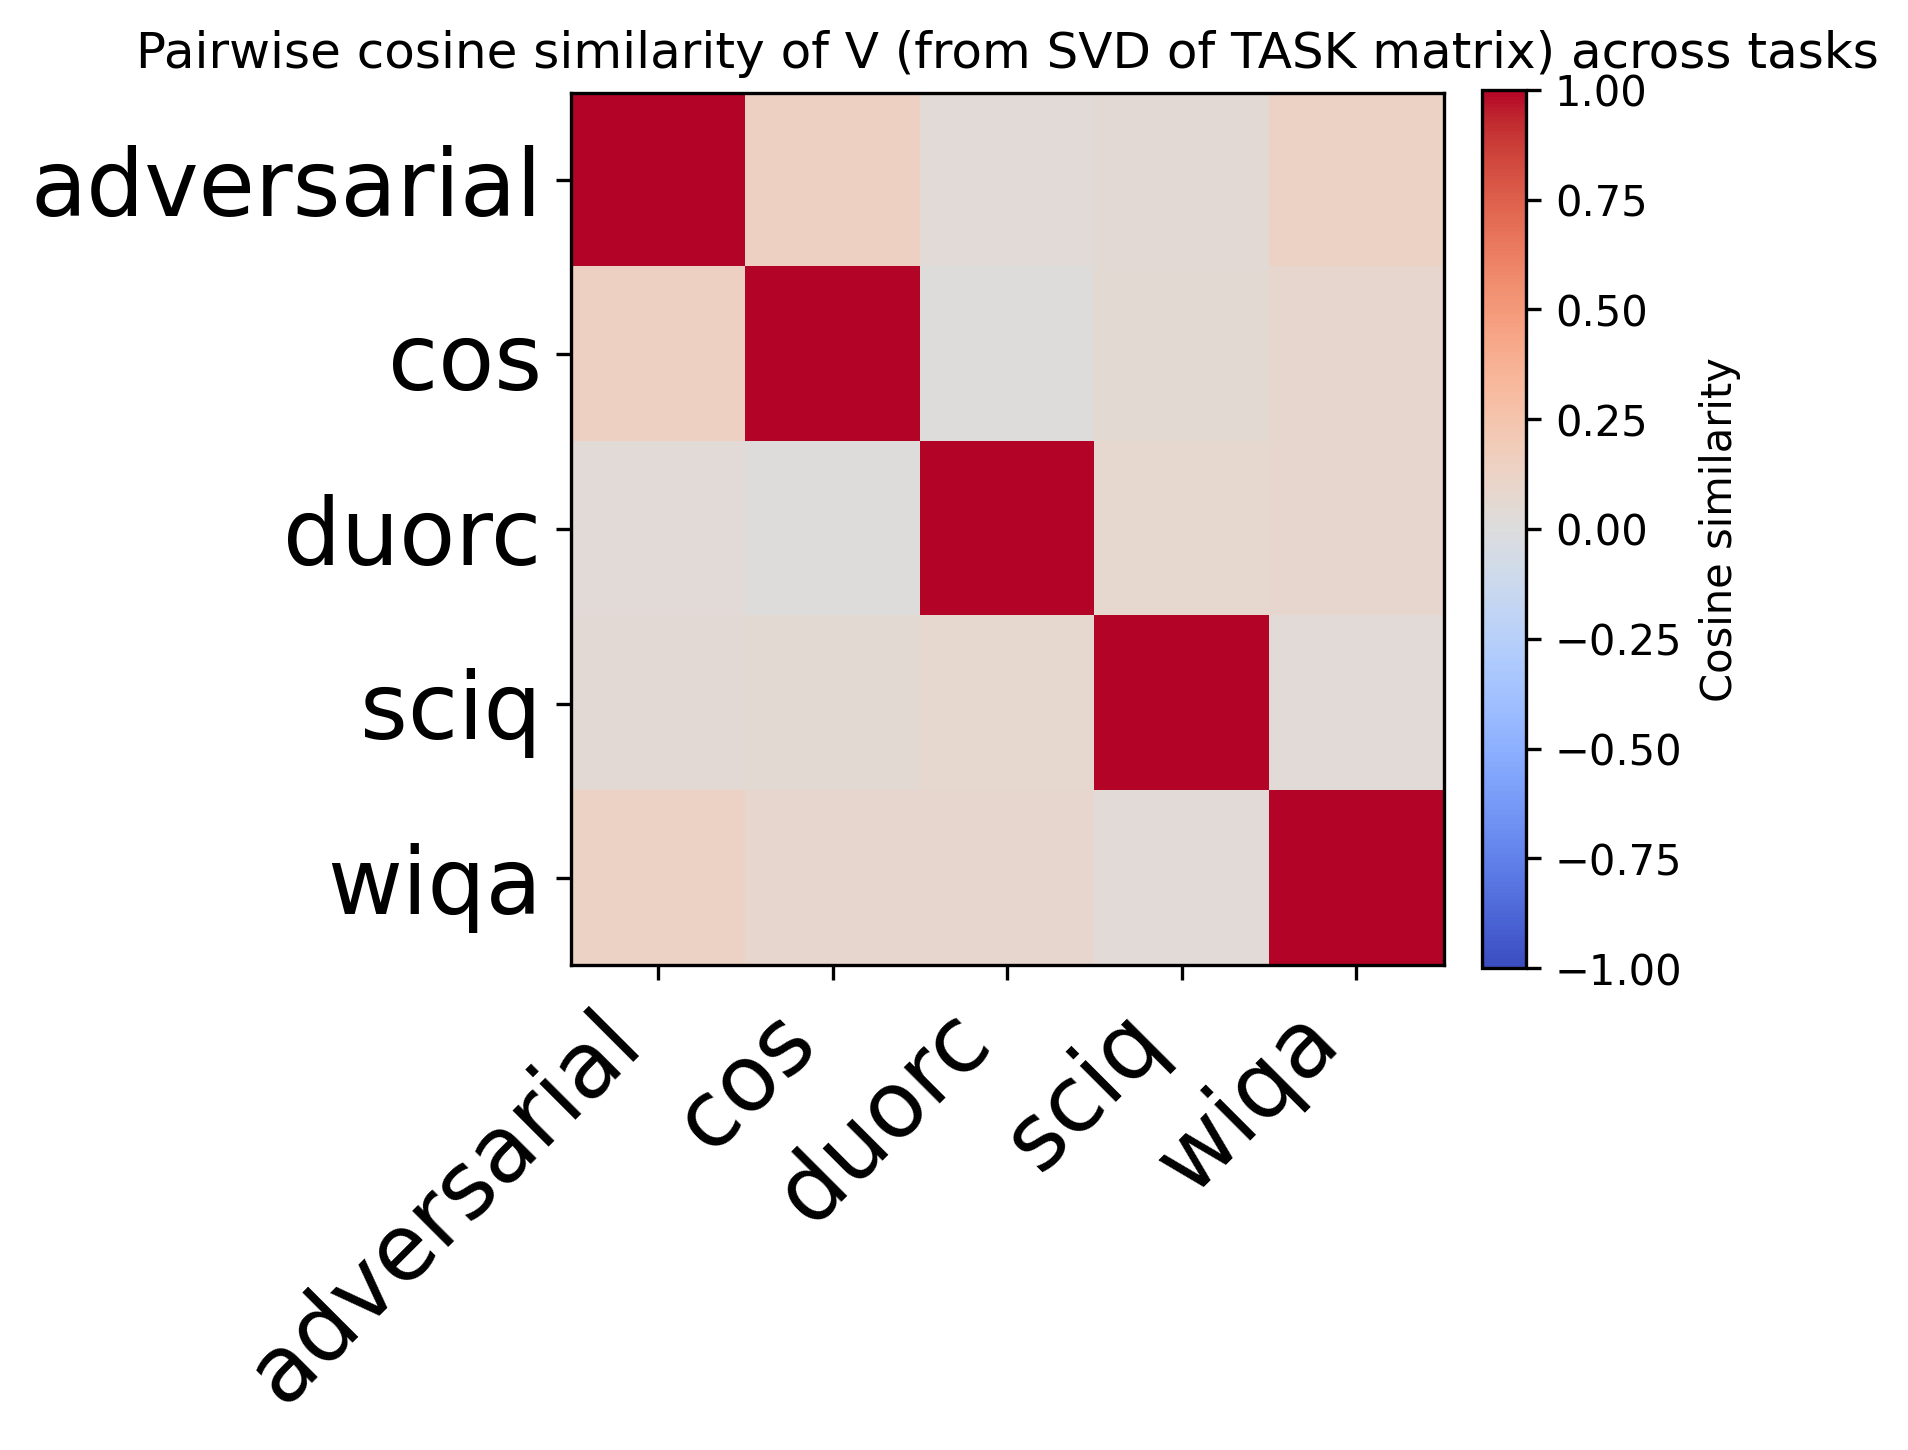
\includegraphics[width=0.30\textwidth]{fig/cpmergeafter_svd_v_cosine_similarity.png}
            % \subcaption{The number of clusters and accuracy (ACC) using Mistral 7B}
        \end{subfigure}
        \caption{(left): pairwise cosine similarity between task experts using CP Eq.5. Each cell compares the task matrices $\Delta_i,\Delta_j$, highlighting cross-task dependence captured by CP's tri-factor interaction. (2)(mid) similarity between the $U$ matrix in SVD decomposition. (3) similarity between the $V$ matrix in SVD. We use layer 0 in the Phi-3 model and compute the cosine similarity across 5 experts.}
        \label{fig:SVD_visualization}
    \end{figure}

We added a quantitative cross-task dependence analysis using the off-diagonal entries of pairwise expert-similarity matrices. Specifically, we compare CP-based task representations (Eq. \ref{eq:cp_form} reconstruction) against SVD-based representations (U, V, and their mean). On the tested layer, CP-vs-SVD correlations are only moderate (Pearson: 0.578 vs U, 0.486 vs V, 0.576 vs (U+V)/2; Spearman: 0.305, 0.353, 0.377), and the average absolute discrepancy is non-trivial (0.204). This indicates that SVD and CP induce meaningfully different cross-task dependence structures rather than being equivalent. We also observe that SVD dependence is imbalanced across factors (mean off-diagonal: U=0.348, V=0.068), while CP task vector captures a coherent dependence pattern at the full task-matrix level (0.349). These quantitative results strengthen our motivation for CPD: it models cross-task interactions through a shared tri-factor structure and preserves dependence information beyond what is captured by SVD basis components alone.

\begin{figure}[h]
    \centering
    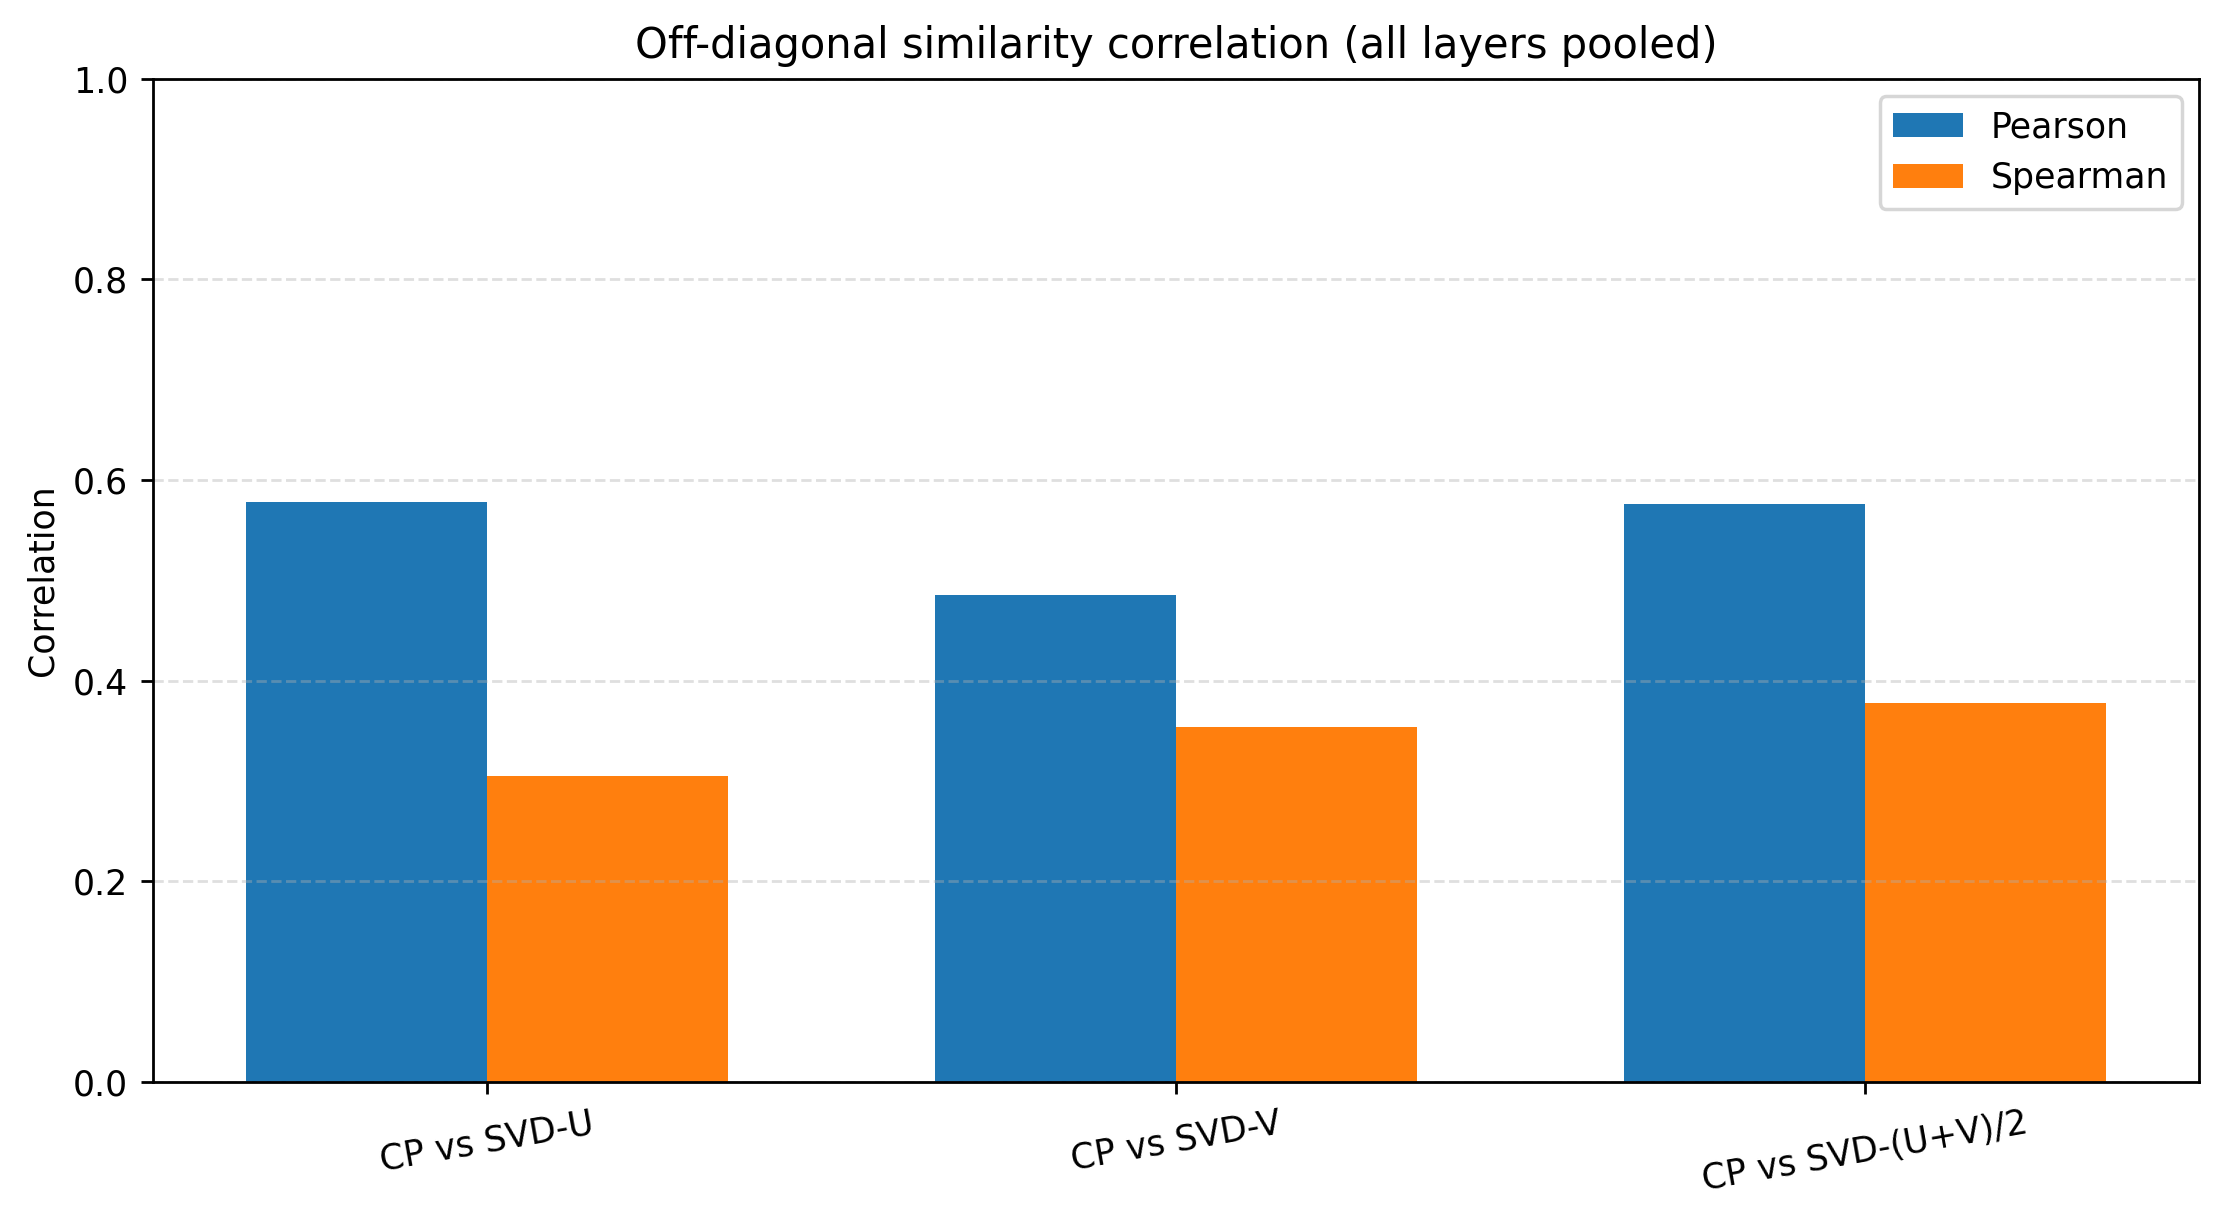
\includegraphics[width=0.8\linewidth]{fig/cpmergeafter_cp_eq5_vs_svd_offdiag_correlation_pooled.png}
    \caption{Quantitative cross-task dependence analysis using the off-diagonal entries of pairwise expert-similarity matrices.}
    \label{fig:placeholder}
\end{figure}


\subsection{Experimental Setting for Flan tasks and Zero-shot downstream tasks.}
\label{sec:exp_setting}

\subsubsection{Implementation Details}

For the CP decomposition in our merging algorithm, we use the open-source Python library Tensorly \footnote{https://tensorly.org/dev/modules/generated/tensorly.decomposition.parafac.html}.  CP decomposition is solved using alternating least squares (ALS) via TensorLy’s parafac solver (random initialization, fixed rank $R$, stopping with tolerance \textit{tol} or maximum iterations \textit{n-iter-max}).


\begin{figure}[h]
    \centering
    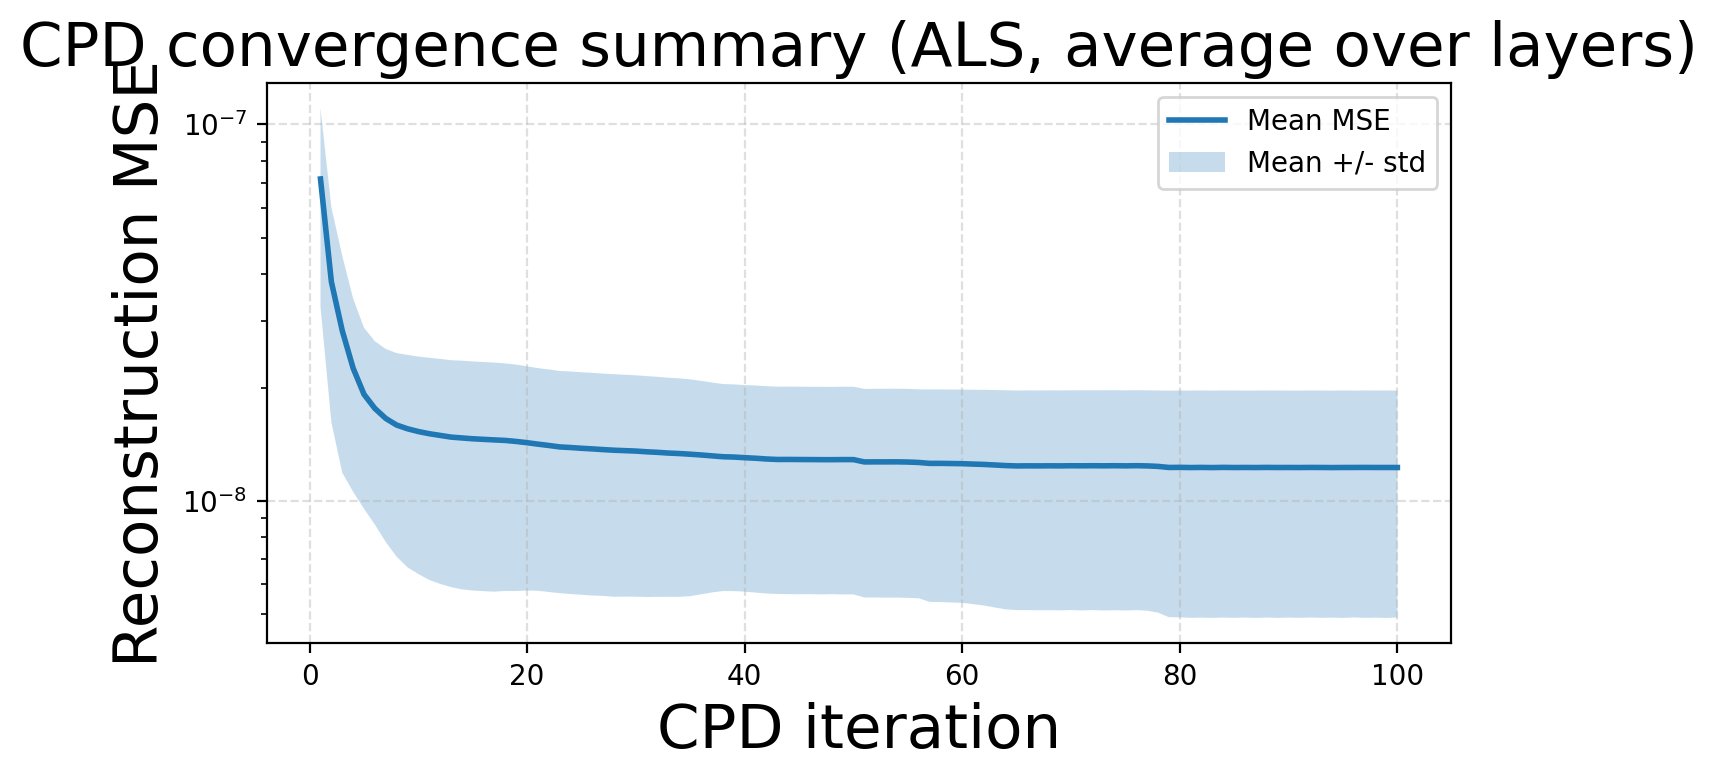
\includegraphics[width=0.8\linewidth]{fig/cpmergeafter_cpd_convergence_summary.png}
    \caption{The CP decomposition based on Phi-3 on LoRA library with 5 experts.}
    \label{fig:placeholder}
\end{figure}

To provide convergence evidence, we now log the reconstruction error at each ALS iteration and report the corresponding reconstruction MSE between the original tensor X and reconstructed tensor $\hat{X}: \text{MSE}_t = ||X - \hat{X}_t||_F^2 / |X|$ (equivalently computed from TensorLy’s relative reconstruction error trajectory). We include both per-layer convergence curves and an averaged summary across layers (mean ± std over layers), and observe stable monotonic error reduction with saturation after a modest number of iterations. These results support that the CPD optimization in Step 5 is numerically well-behaved and convergent in our setting.

% \begin{figure}[h]
%         \centering
%         \begin{subfigure}
%             \centering
%             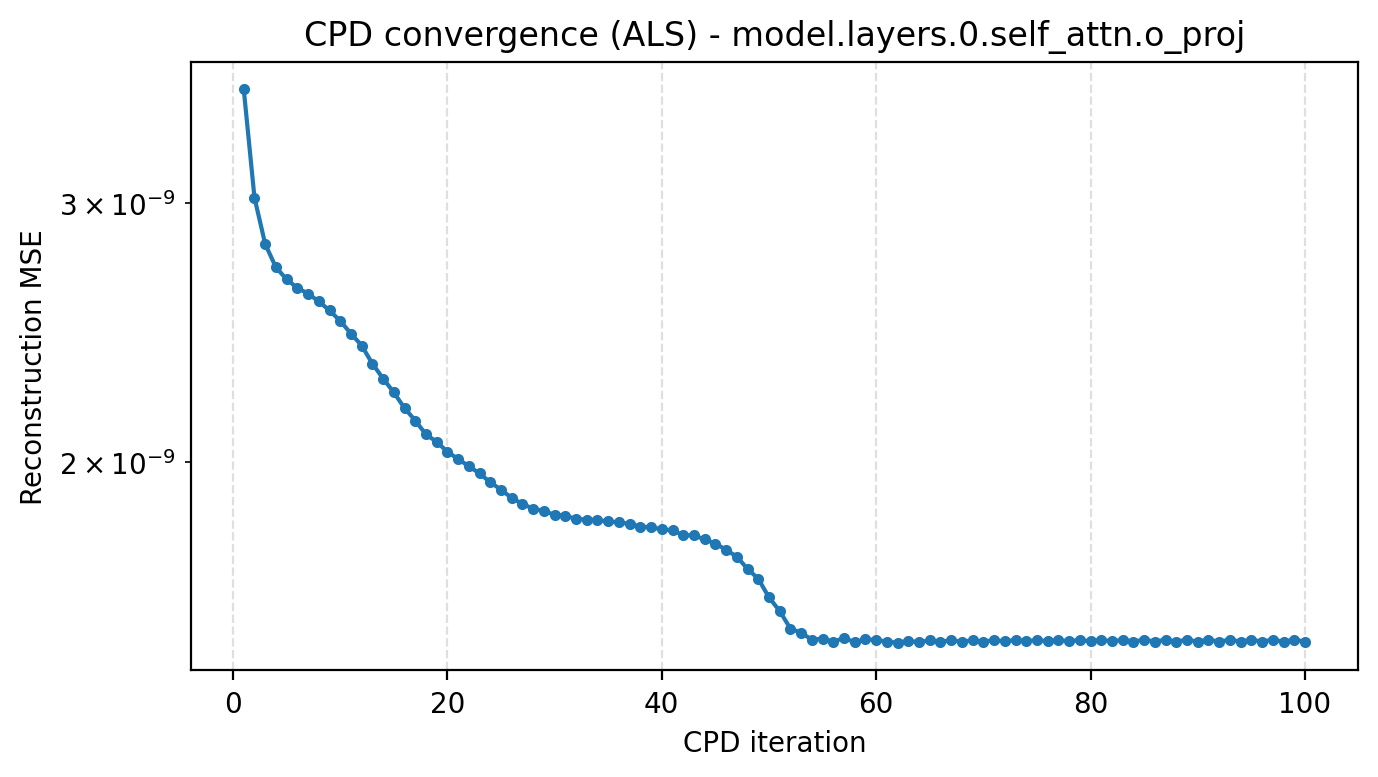
\includegraphics[width=0.3\textwidth]{fig/cpmergeafter_cpd_convergence_model.layers.0.self_attn.o_proj.png}
%             % \subcaption{The number of clusters and accuracy (ACC) using Phi-3 3B}
%         \end{subfigure}
%         \hfill
%         \begin{subfigure}
%             \centering
%             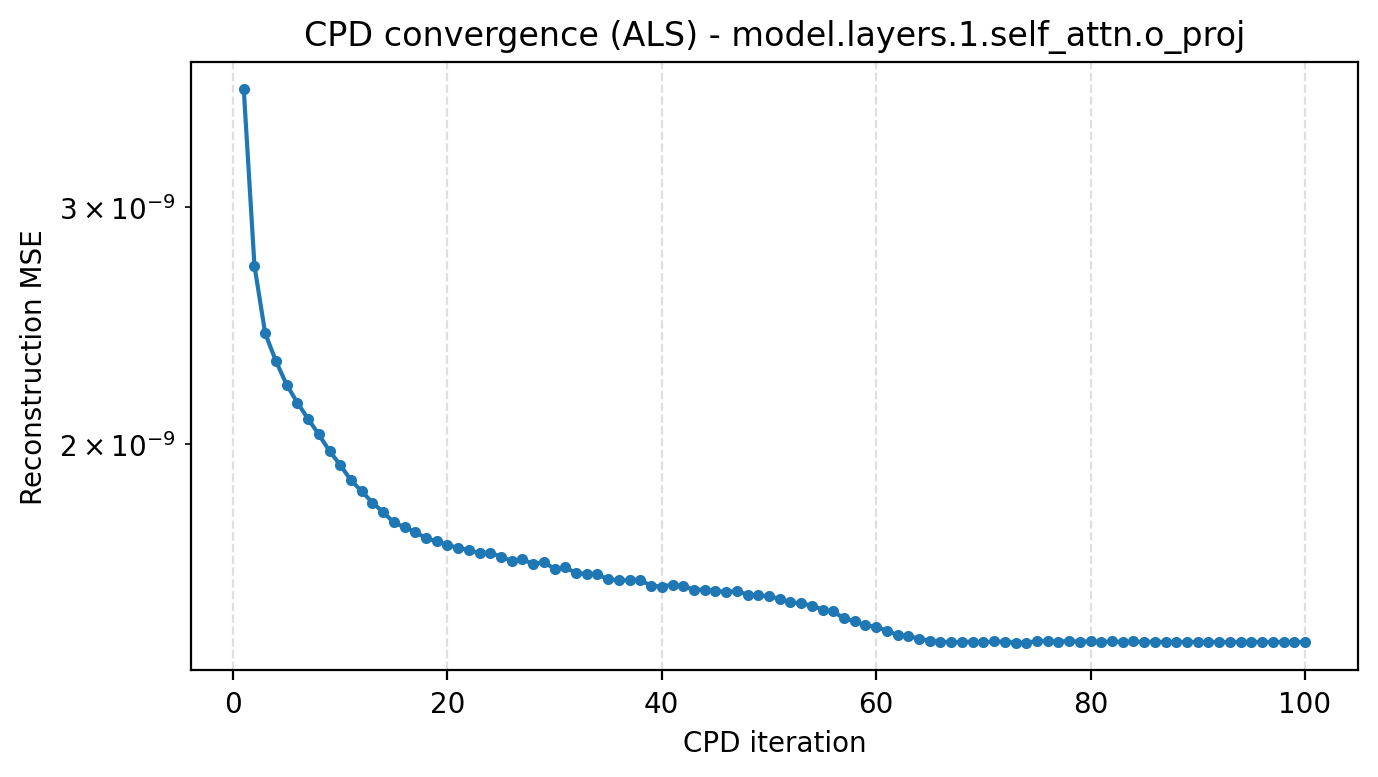
\includegraphics[width=0.3\textwidth]{fig/cpmergeafter_cpd_convergence_model.layers.1.self_attn.o_proj.png}
%             % \subcaption{The number of clusters and accuracy (ACC) using Mistral 7B}
%         \end{subfigure}
%         \hfill
%         \begin{subfigure}
%             \centering
%             \includegraphics[width=0.3\textwidth]{
%                 fig/cpmergeafter_cpd_convergence_model.layers.1.self_attn.o_proj.png}
%             % \subcaption{Clustering based on the sentence embedding. We visualize  100 samples in each cluster.} 
%         \end{subfigure}
%         \caption{(left). The number of clusters and accuracy (ACC) using Phi-3 3B. Cluster analysis. The number of clusters and accuracy (ACC) using Mistral 7B. Clustering based on the sentence embedding. We visualize  100 samples in each cluster.}
%         \label{fig:cluster_performance}
%     \end{figure}


\subsubsection{Datasets and Running Environment Setting}

To enhance the LLM with various abilities for the above tasks, we construct a collection of LoRA adapters on diverse tasks. We use the FlanV2, an instruction-tuning dataset designed to scale both task diversity and model size, which has been shown to improve model performance significantly \citep{chung2024scaling}. We train each LoRA adapter independently, enabling it to specialize in a specific task. Finally, we select 256 tasks \citep{longpre2023flan}, with the majority derived from P3 \citep{bach2022promptsource} and Flan2021 \citep{wei2021finetuned}. 

To evaluate the effectiveness of our approach across different backbone models, we conduct experiments using Phi-3 \citep{abdin2024phi}, and Mistral-7B(mistralai/Mistral-7B-v0.1) \citep{jiang2023mistral}. In all cases, we apply LoRA adapters exclusively to the attention layers. Unless stated otherwise, our multi-task training and single-task adaptation scenarios employ a LoRA rank of 4, a dropout rate of 0.05, and a learning rate of 1e-4. Each LoRA adapter is trained for 5 epochs on either an H100 or A100 GPU. For the clustering step, we use the \texttt{sentence-transformers/sentence-t5-xxl} model for encoding. Given the typically large size of the dataset, we sample 20\% of the data to train the k-means algorithm and then use the resulting clusters to predict labels for all samples.

\subsubsection{10 Held-in and 3 Held out task names}
\label{sec:10_held_in}

There are 256 pre-trained LoRA adapters used in \cite{ostapenko2024towards}. We randomly select 10 tasks as the held-in tasks and 3 tasks as the held-out tasks, followed by \cite{arnob2025exploring}. 

\paragraph{Held-in tasks}

\begin{itemize}
    \item wiqa\_what\_is\_the\_final\_step\_of\_the\_following\_process
    \item sciq\_Multiple\_Choice
    \item adversarial\_qa\_droberta\_answer\_the\_following\_q
    \item duorc\_SelfRC\_question\_answering
    \item cos\_e\_v1\_11\_description\_question\_option\_id
    \item wiki\_qa\_Is\_This\_True\_
    \item quail\_description\_context\_question\_text
    \item wiki\_hop\_original\_explain\_relation
    \item duorc\_ParaphraseRC\_build\_story\_around\_qa
    \item yelp\_polarity\_reviews\_0\_2\_0
\end{itemize}

\paragraph{3 held-out tasks}
\begin{itemize}
    \item glue\_sst2\_2\_0\_0
    \item dream\_read\_the\_following\_conversation\_and\_answer\_the\_question
    \item race\_middle\_Read\_the\_article\_and\_answer\_the\_question\_no\_option\_
\end{itemize}

\subsection{Cross layer analysis.}



\begin{figure}[h]
    \centering
    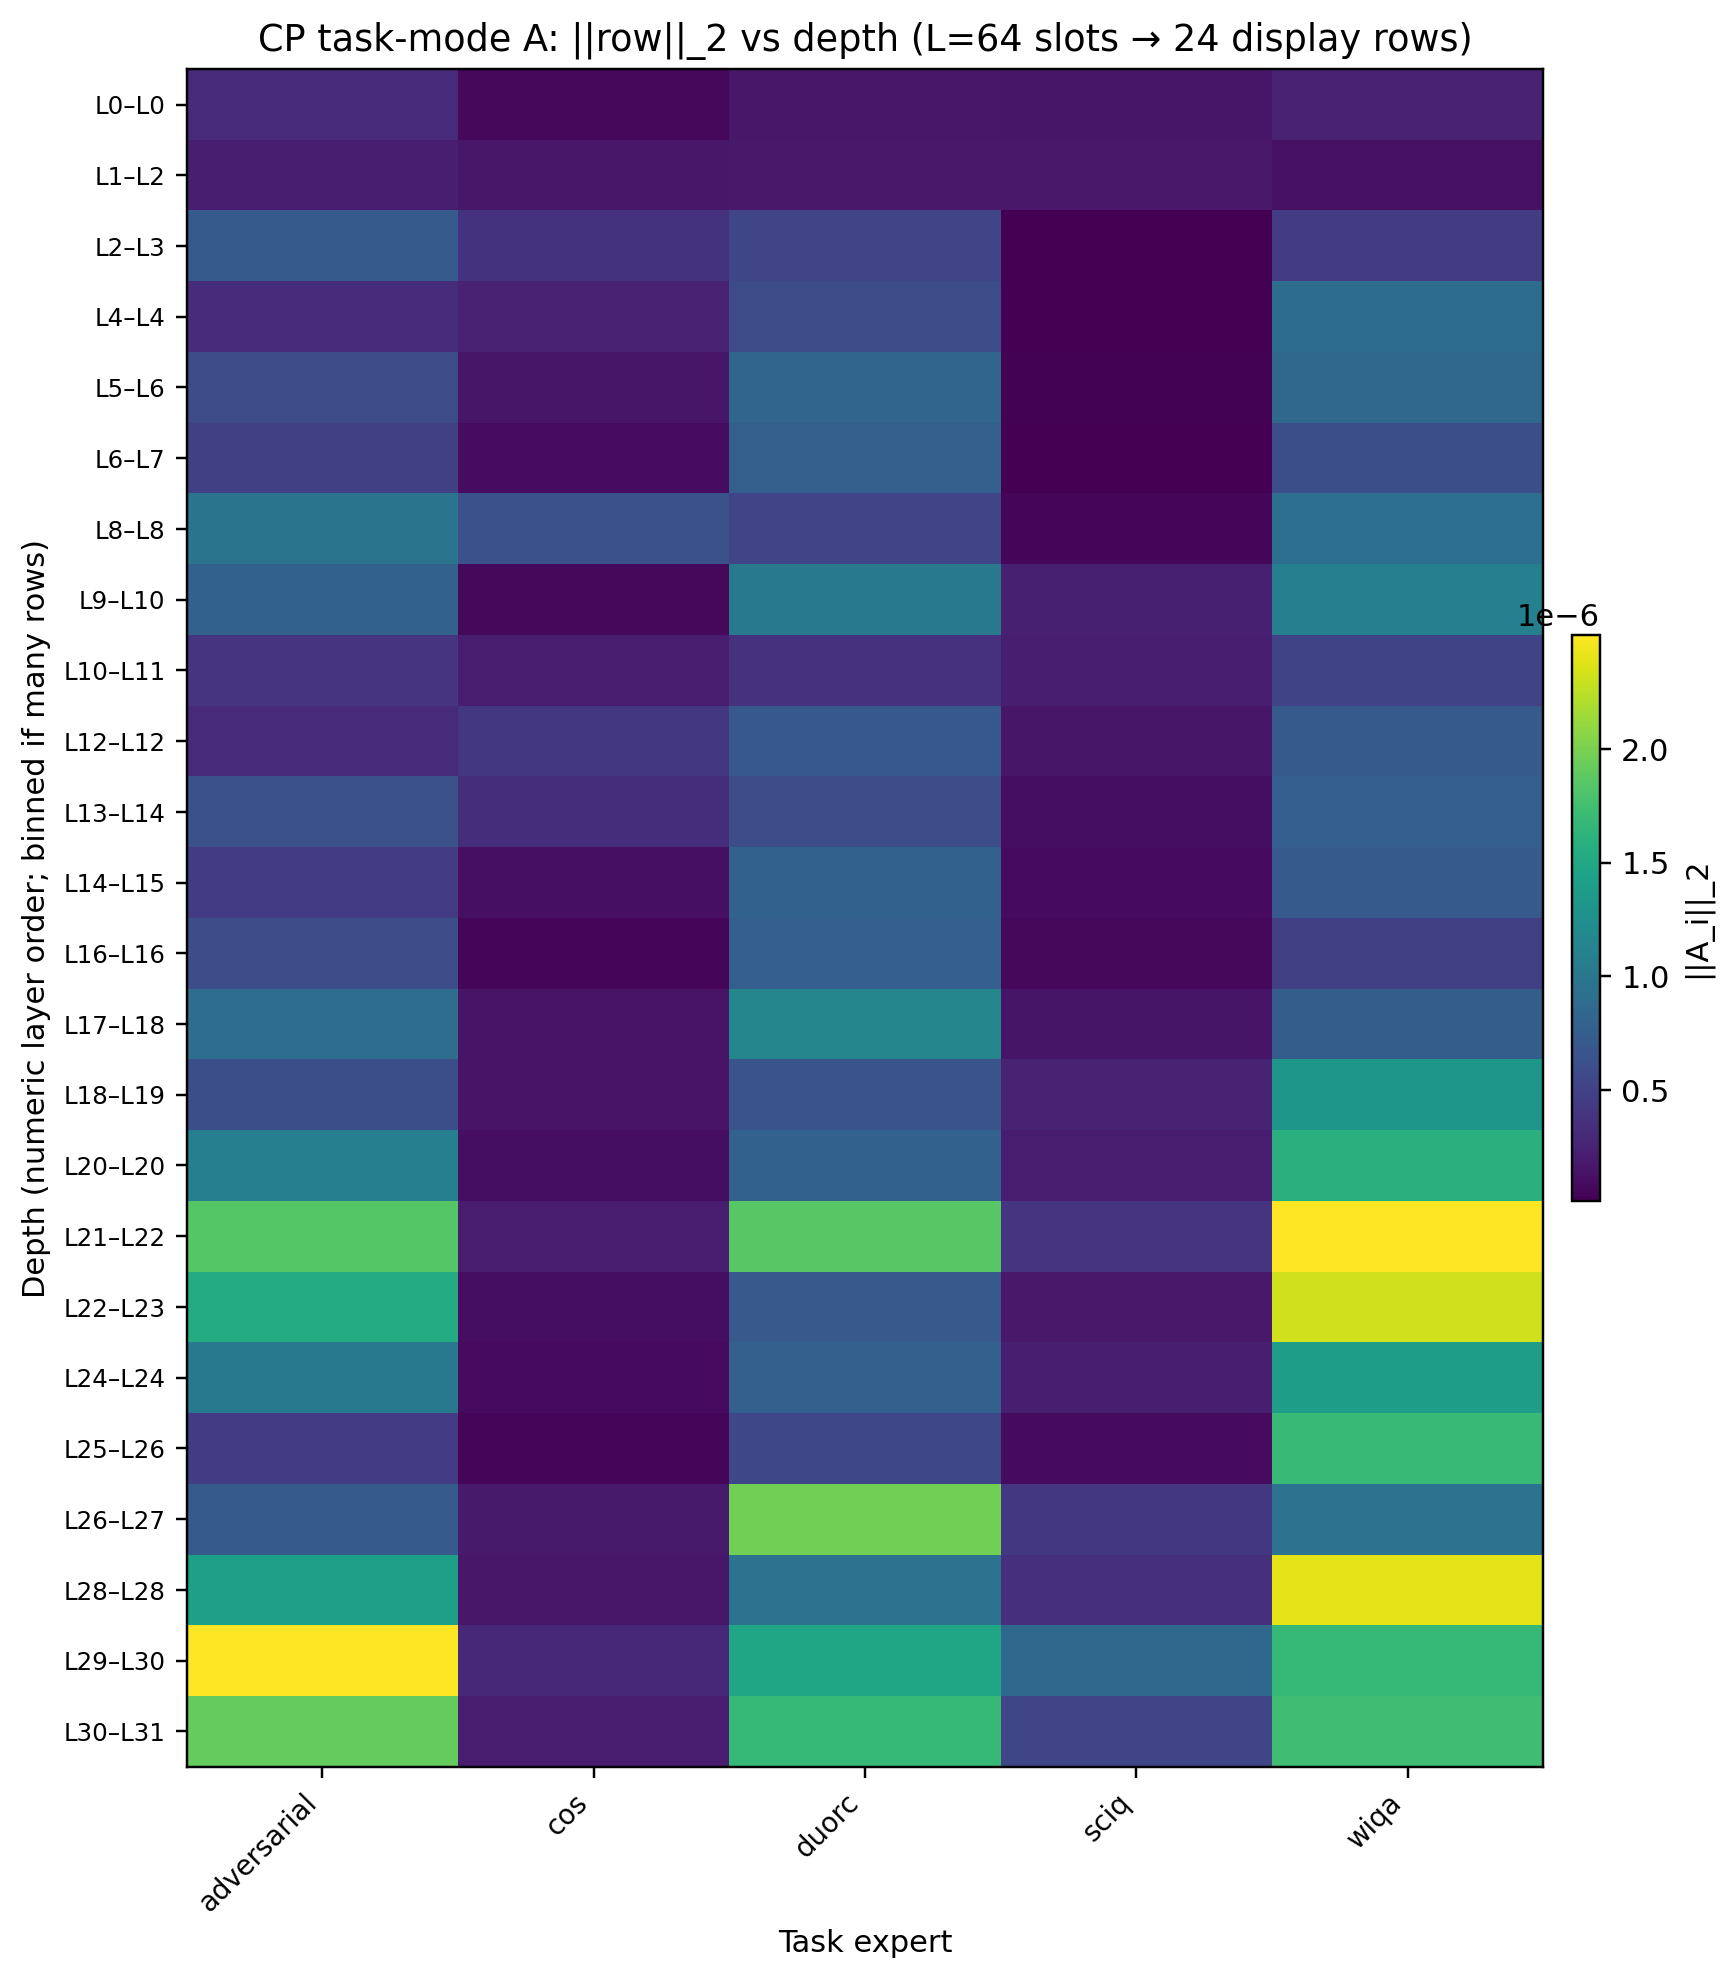
\includegraphics[width=0.5\linewidth]{fig/cpmergeafter_cross_layer_task_A_l2_heatmap.png}
    \caption{L2 norm of each task row vs layer.}
    \label{fig:l2_norm_cross_layer}
\end{figure}

We summarize each task’s CP mixture at a layer by the L2 norm of its row in A and the entropy of the magnitude-normalized mixture (how peaked vs diffuse the rank weights are). As shown in the Figure \ref{fig:l2_norm_cross_layer}. The heatmap shows that task influence is not uniform across depth: some tasks remain small across most layer–projection slots, while others concentrate in later blocks (notably deeper o\_proj / qkv\_proj rows), indicating that the learned decomposition reflects structured depth dependence rather than i.i.d. local noise. This directly addresses whether “importance” is constant: it is layer- and projection-dependent, with interpretable bands rather than flat profiles.


\begin{figure}[h]
    \centering
    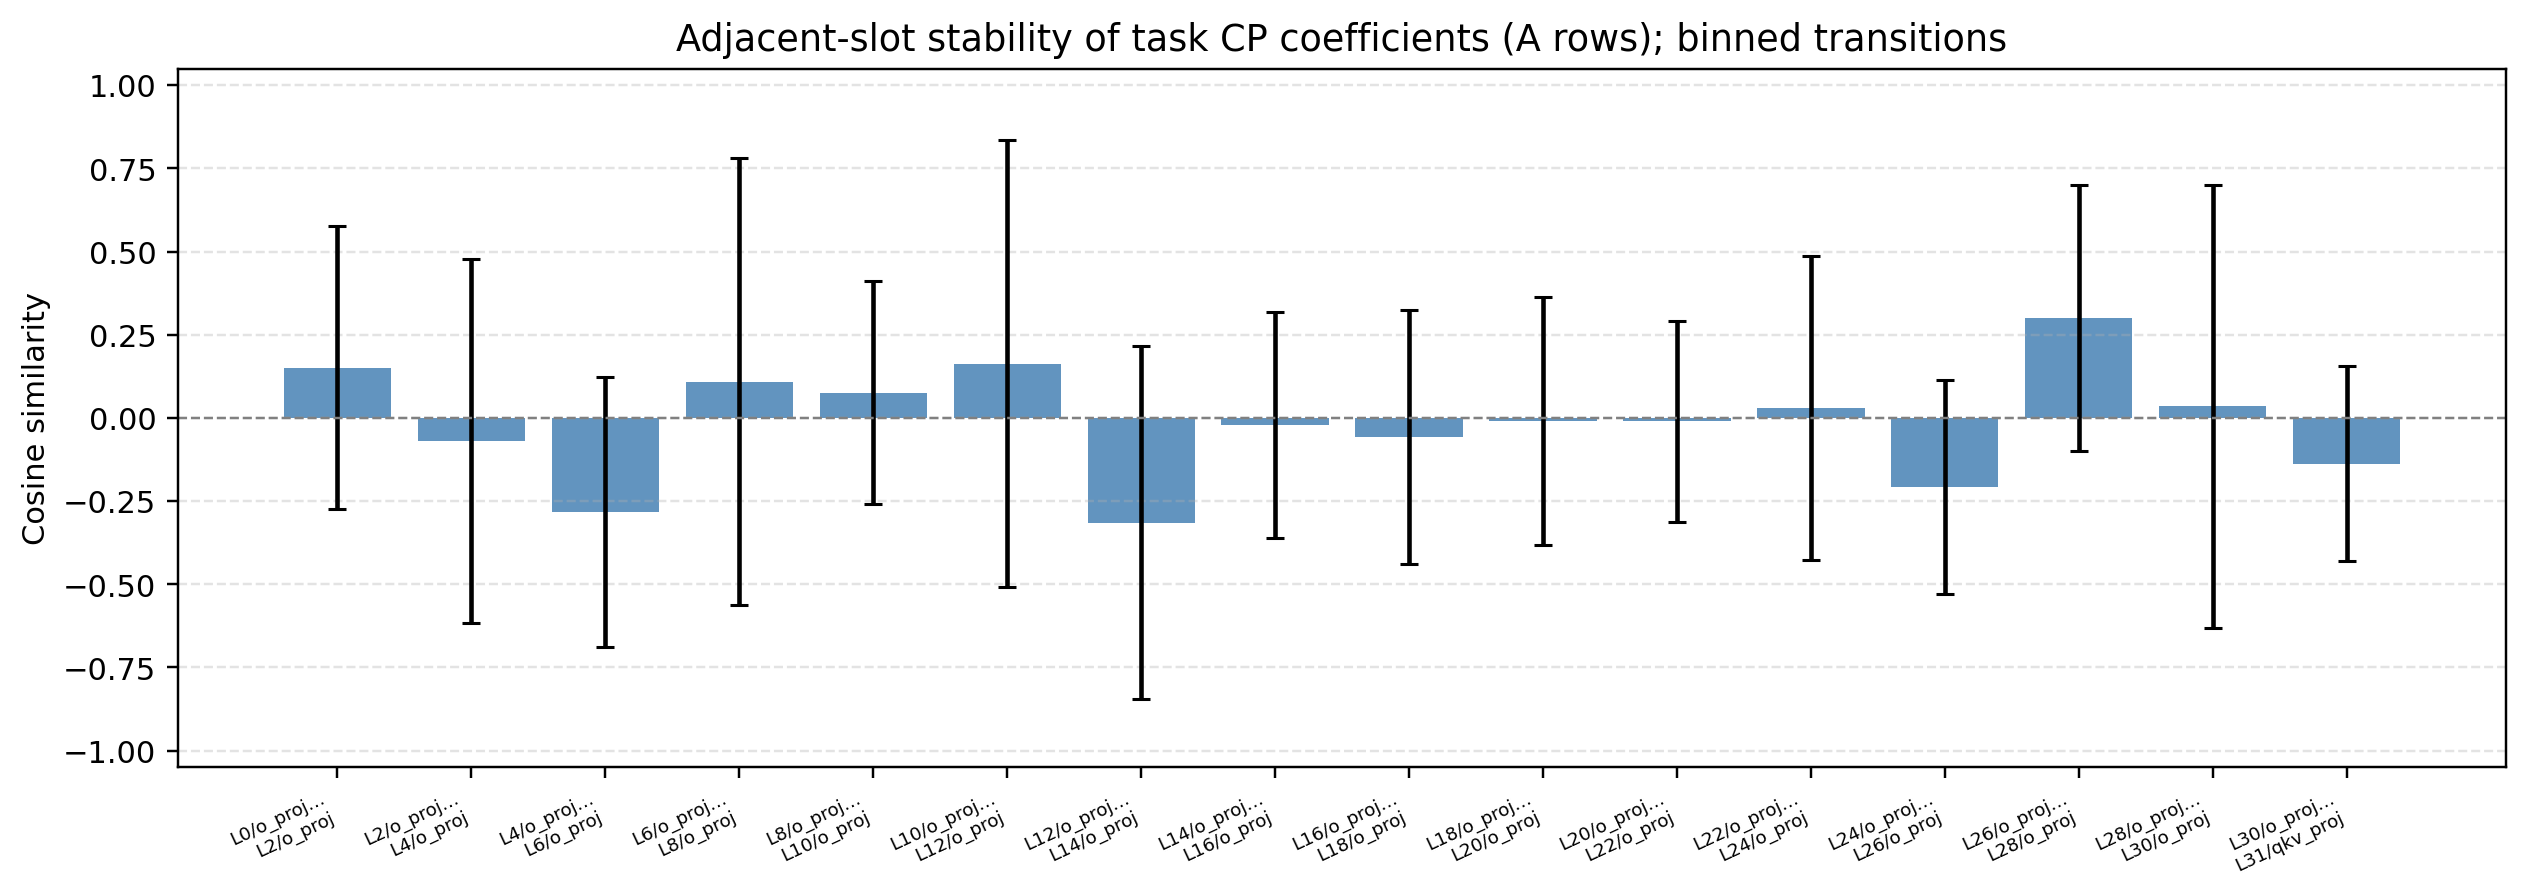
\includegraphics[width=\linewidth]{fig/cpmergeafter_cross_layer_task_A_adjacent_cosine.png}
    \caption{Adjacent-slot stability of task CP coefficients (A rows).}
    \label{fig:adjacent_cross_layer}
\end{figure}

In Figure \ref{fig:adjacent_cross_layer}, we measure the cosine similarity between its A row at layer L and at the next processed layer, then report the mean ± std across tasks for each adjacent pair. The resulting curve is mixed: several transitions show positive mean alignment (e.g. L10 o\_proj → L10 qkv\_proj at 0.535 mean cosine, L27 qkv\_proj → L28 o\_proj at 0.454), while others are near zero or negative with large standard deviations (often 0.3–0.9), reflecting that (i) o\_proj and qkv\_proj are different operators with different induced geometry, and (ii) CP factors have scale/sign/permutation non-identifiability, so A is not guaranteed to be pointwise stable under independent per-layer fits. We therefore interpret this plot as a sanity check for continuity under our layer-wise fitting protocol, not as a claim of a single global latent “task embedding” shared verbatim at every depth.


\begin{figure}[h]
    \centering
    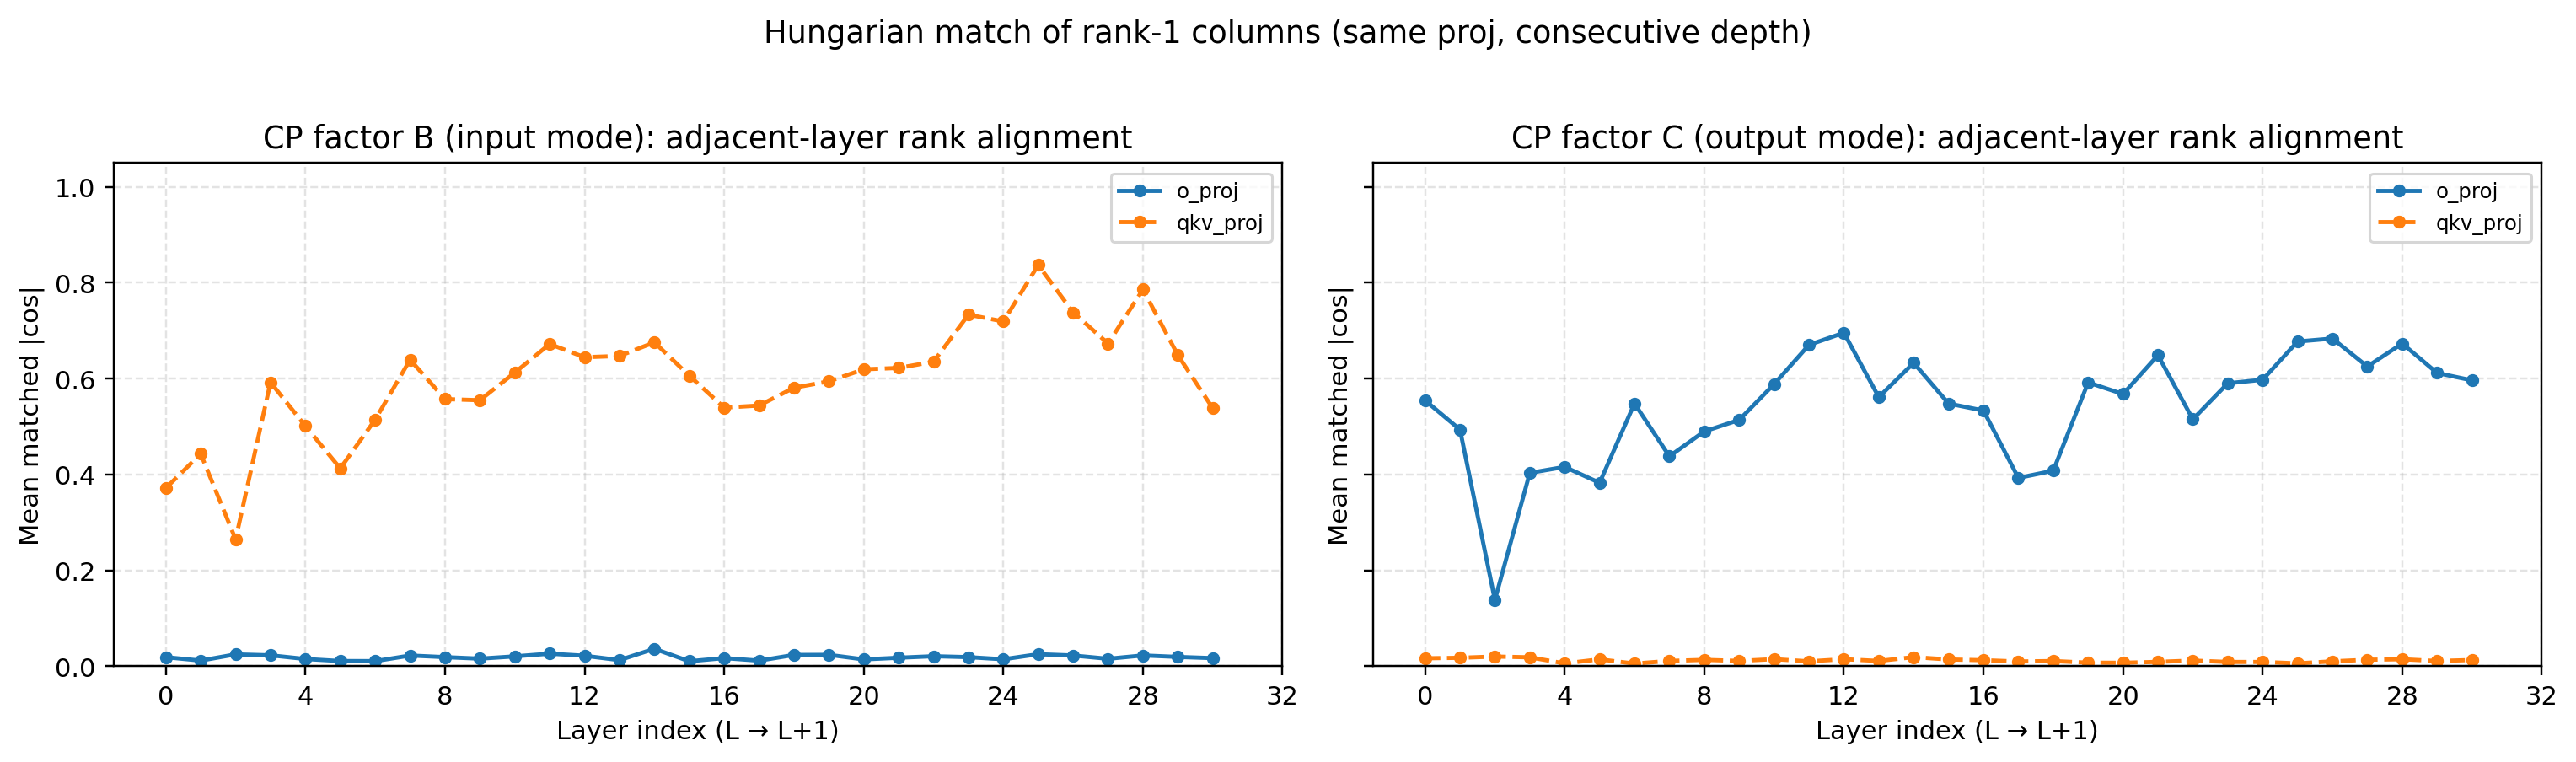
\includegraphics[width=\linewidth]{fig/cpmergeafter_cross_layer_BC_rank_alignment_adjacent.png}
    \caption{Rank-1 feature across depth. |cos| means the absolute value of the cosine similarity between two column vectors of the CP factor matrices B or C (after each column is L2-normalized).}
    \label{fig:bc_bank}
\end{figure}

Because CP rank order is arbitrary within each layer, we report Hungarian alignment of normalized factor columns between consecutive transformer indices within the same projection family (o\_proj vs qkv\_proj). As shown in the Figure \ref{fig:bc_bank}, the results are split by factor and projection: for B on qkv\_proj, matched |cos| between adjacent layers is typically moderate to high (often 0.37–0.84, e.g. peak ~0.84 at L25→L26), suggesting recurring rank-1 directions in the input mode along depth for QKV adapters. For B on o\_proj, matched |cos| is much lower (often ~0.01–0.04), indicating that rank labels are not vertically stable for output projections under independent CPD—consistent with known CP identifiability limits. For C, o\_proj shows higher adjacent matched similarity than qkv\_proj (e.g. many o\_proj pairs in the 0.4–0.7 range vs qkv\_proj often ~0.006–0.02), so “vertical semantics” of rank-1 components must be stated separately for each factor and each projection type.
    

    \subsection{Clusterized LoRA Library (C-LoRA)}
    \label{sec:clora}

    As noted in \cite{ostapenko2024towards}, LoRA similarity can contribute to positive transfer. Their approach clusters tasks based on LoRA similarity, requiring the \textit{task ID} for each example and the pre-training of a collection of LoRA adapters before clustering. In contrast, we argue that text-level clustering is more convenient while achieving competitive results. As shown in Fig. \ref{fig:cluster_performance}, we select 100 examples per cluster and visualize their embeddings. The embeddings reveal that similar texts are grouped into the same clusters, demonstrating the quality of our embedding representations.

    To mitigate task conflicts at the \textit{text-level}, we train each \textit{expert}
    on a collection of similar tasks. This is achieved by clustering instructions
    and partitioning the training data into multiple clusters without requiring manual
    intervention. Clustering input texts into several groups can reduce task
    interference by allowing the model to adapt its task adapters or
    representations to distinct subsets of data with similar characteristics. Formally,
    let $E(\cdot)$ denote a pretrained sentence encoder. For each data sample,
    the sentence representation of an instruction $I_{i}$ is computed as
    $e_{i}=E(I_{i})$. We then apply the k-means algorithm to cluster all instruction
    embeddings $\{e_{i}\}$ in the training dataset into $K$ clusters. We train
    each LoRA adapter based on the instructions from each cluster. For each pre-trained
    weight $W_{0}$, we obtain corresponding LoRA adapters
    $\{A_{i}B_{i},...,A_{K}B_{K}\}$.
    \subsubsection{Clustering to reduce the task interference at the text-level}
    \label{sec:clustering}

    \begin{figure}[h]
        \centering
        \begin{subfigure}
            \centering
            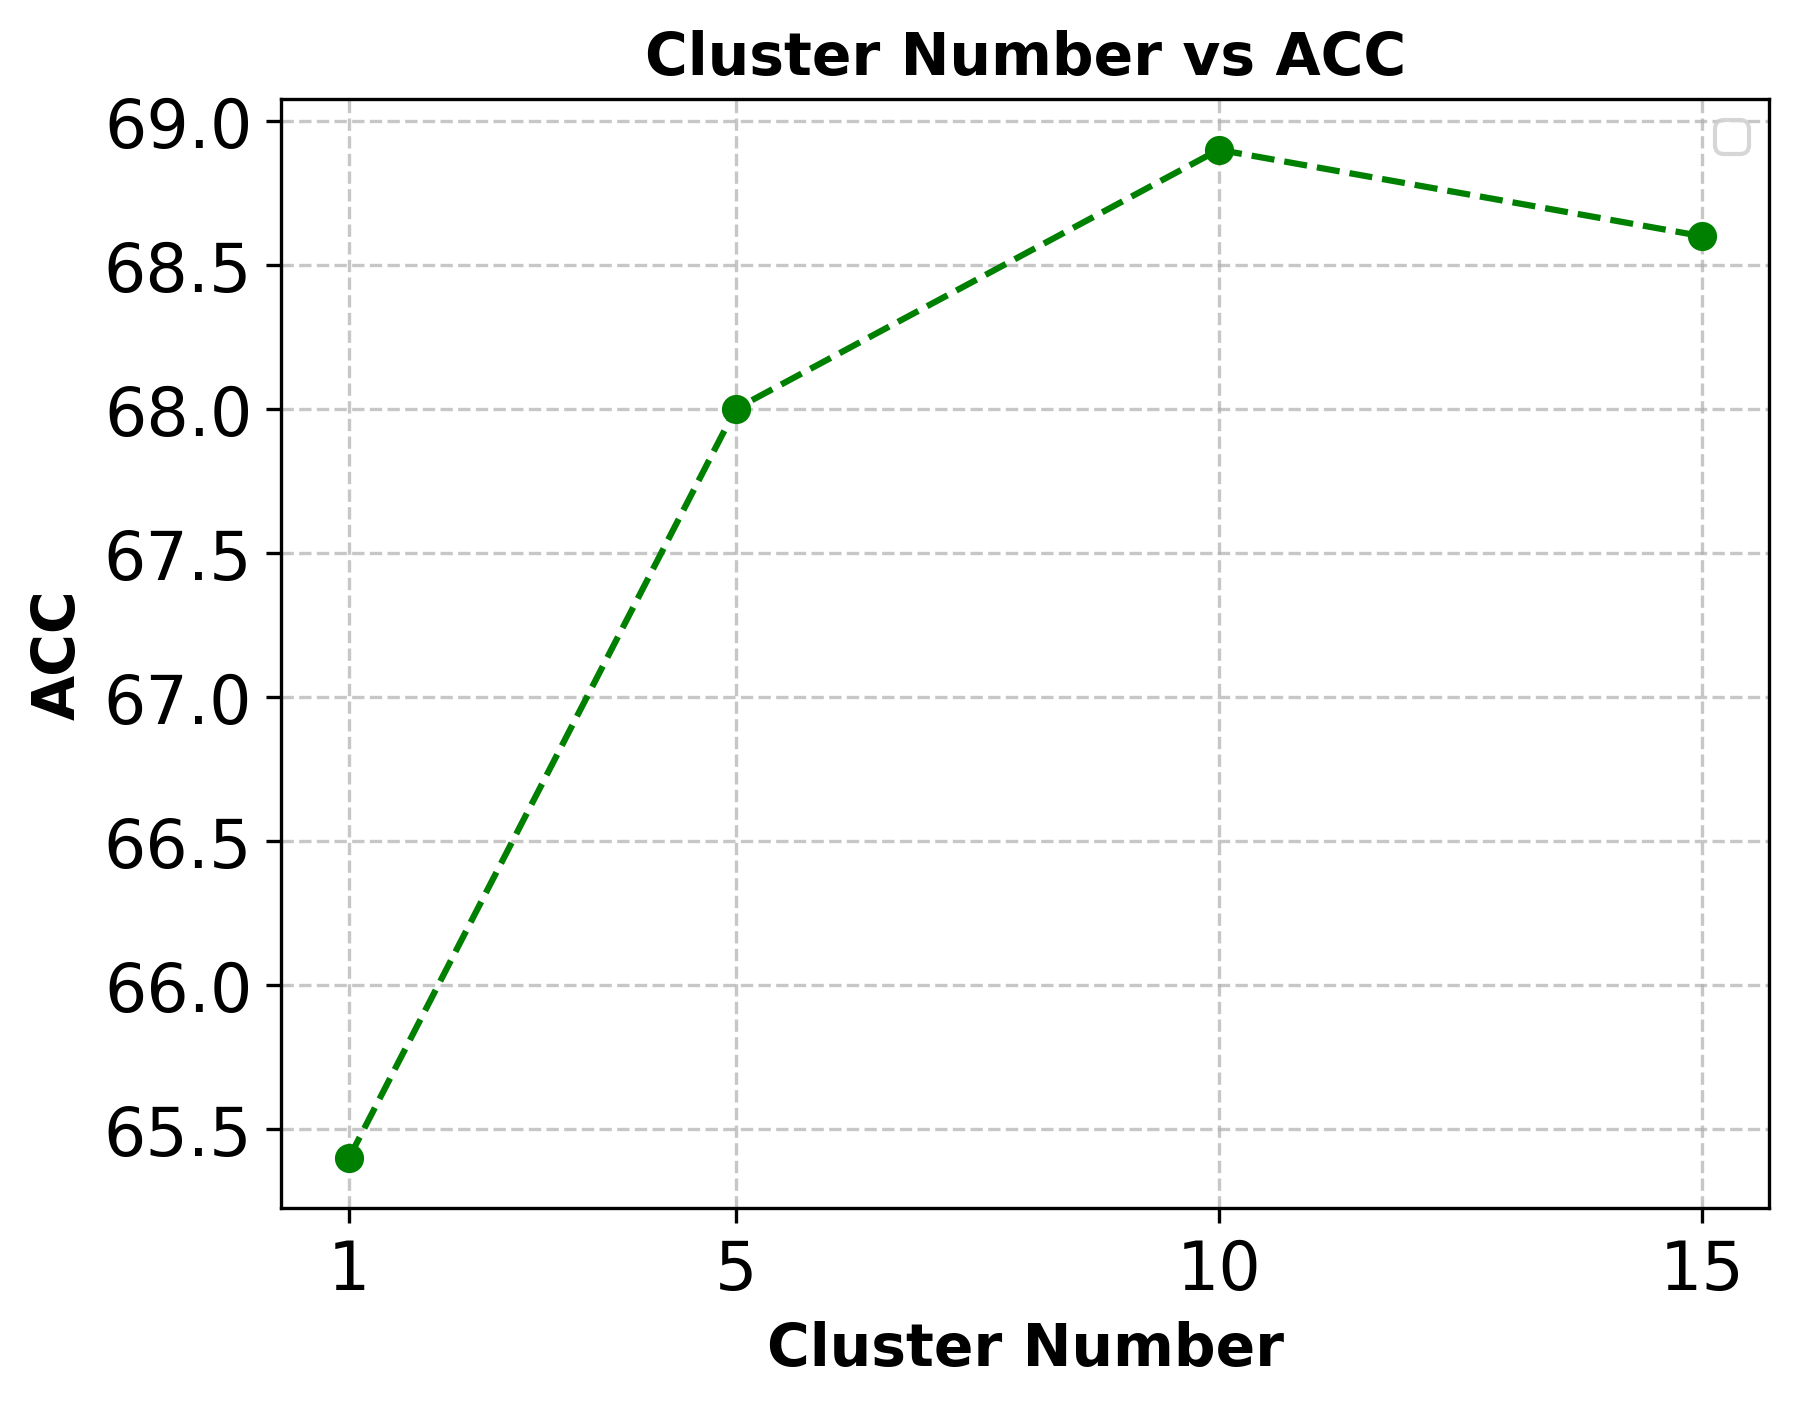
\includegraphics[width=0.3\textwidth]{fig/Cluster_num_vs_ACC_phi3.png}
            % \subcaption{The number of clusters and accuracy (ACC) using Phi-3 3B}
        \end{subfigure}
        \hfill
        \begin{subfigure}
            \centering
            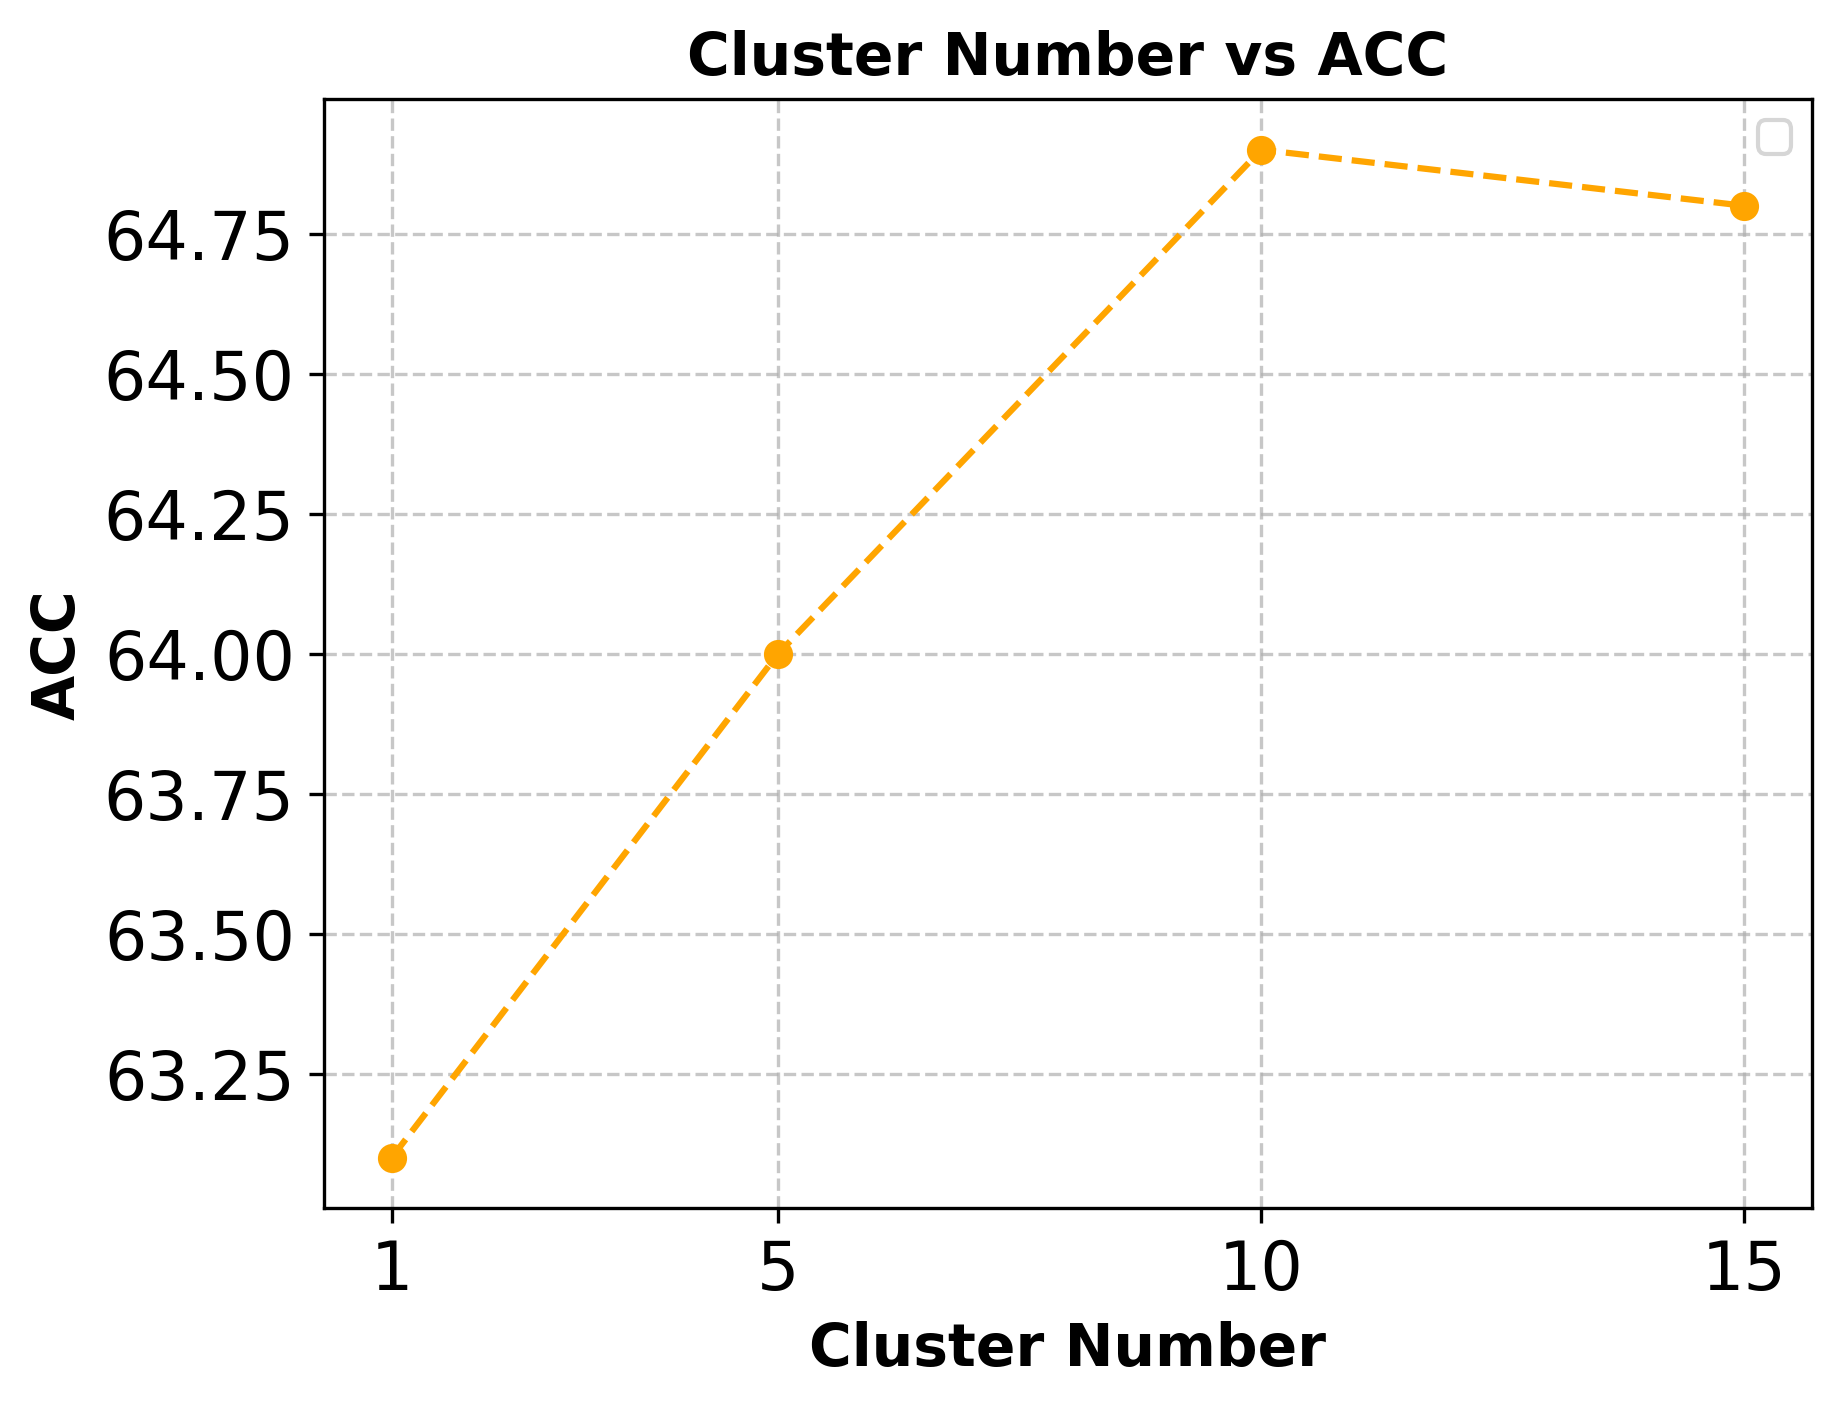
\includegraphics[width=0.3\textwidth]{
                fig/Cluster_num_vs_ACC_mistral.png
            }
            % \subcaption{The number of clusters and accuracy (ACC) using Mistral 7B}
        \end{subfigure}
        \hfill
        \begin{subfigure}
            \centering
            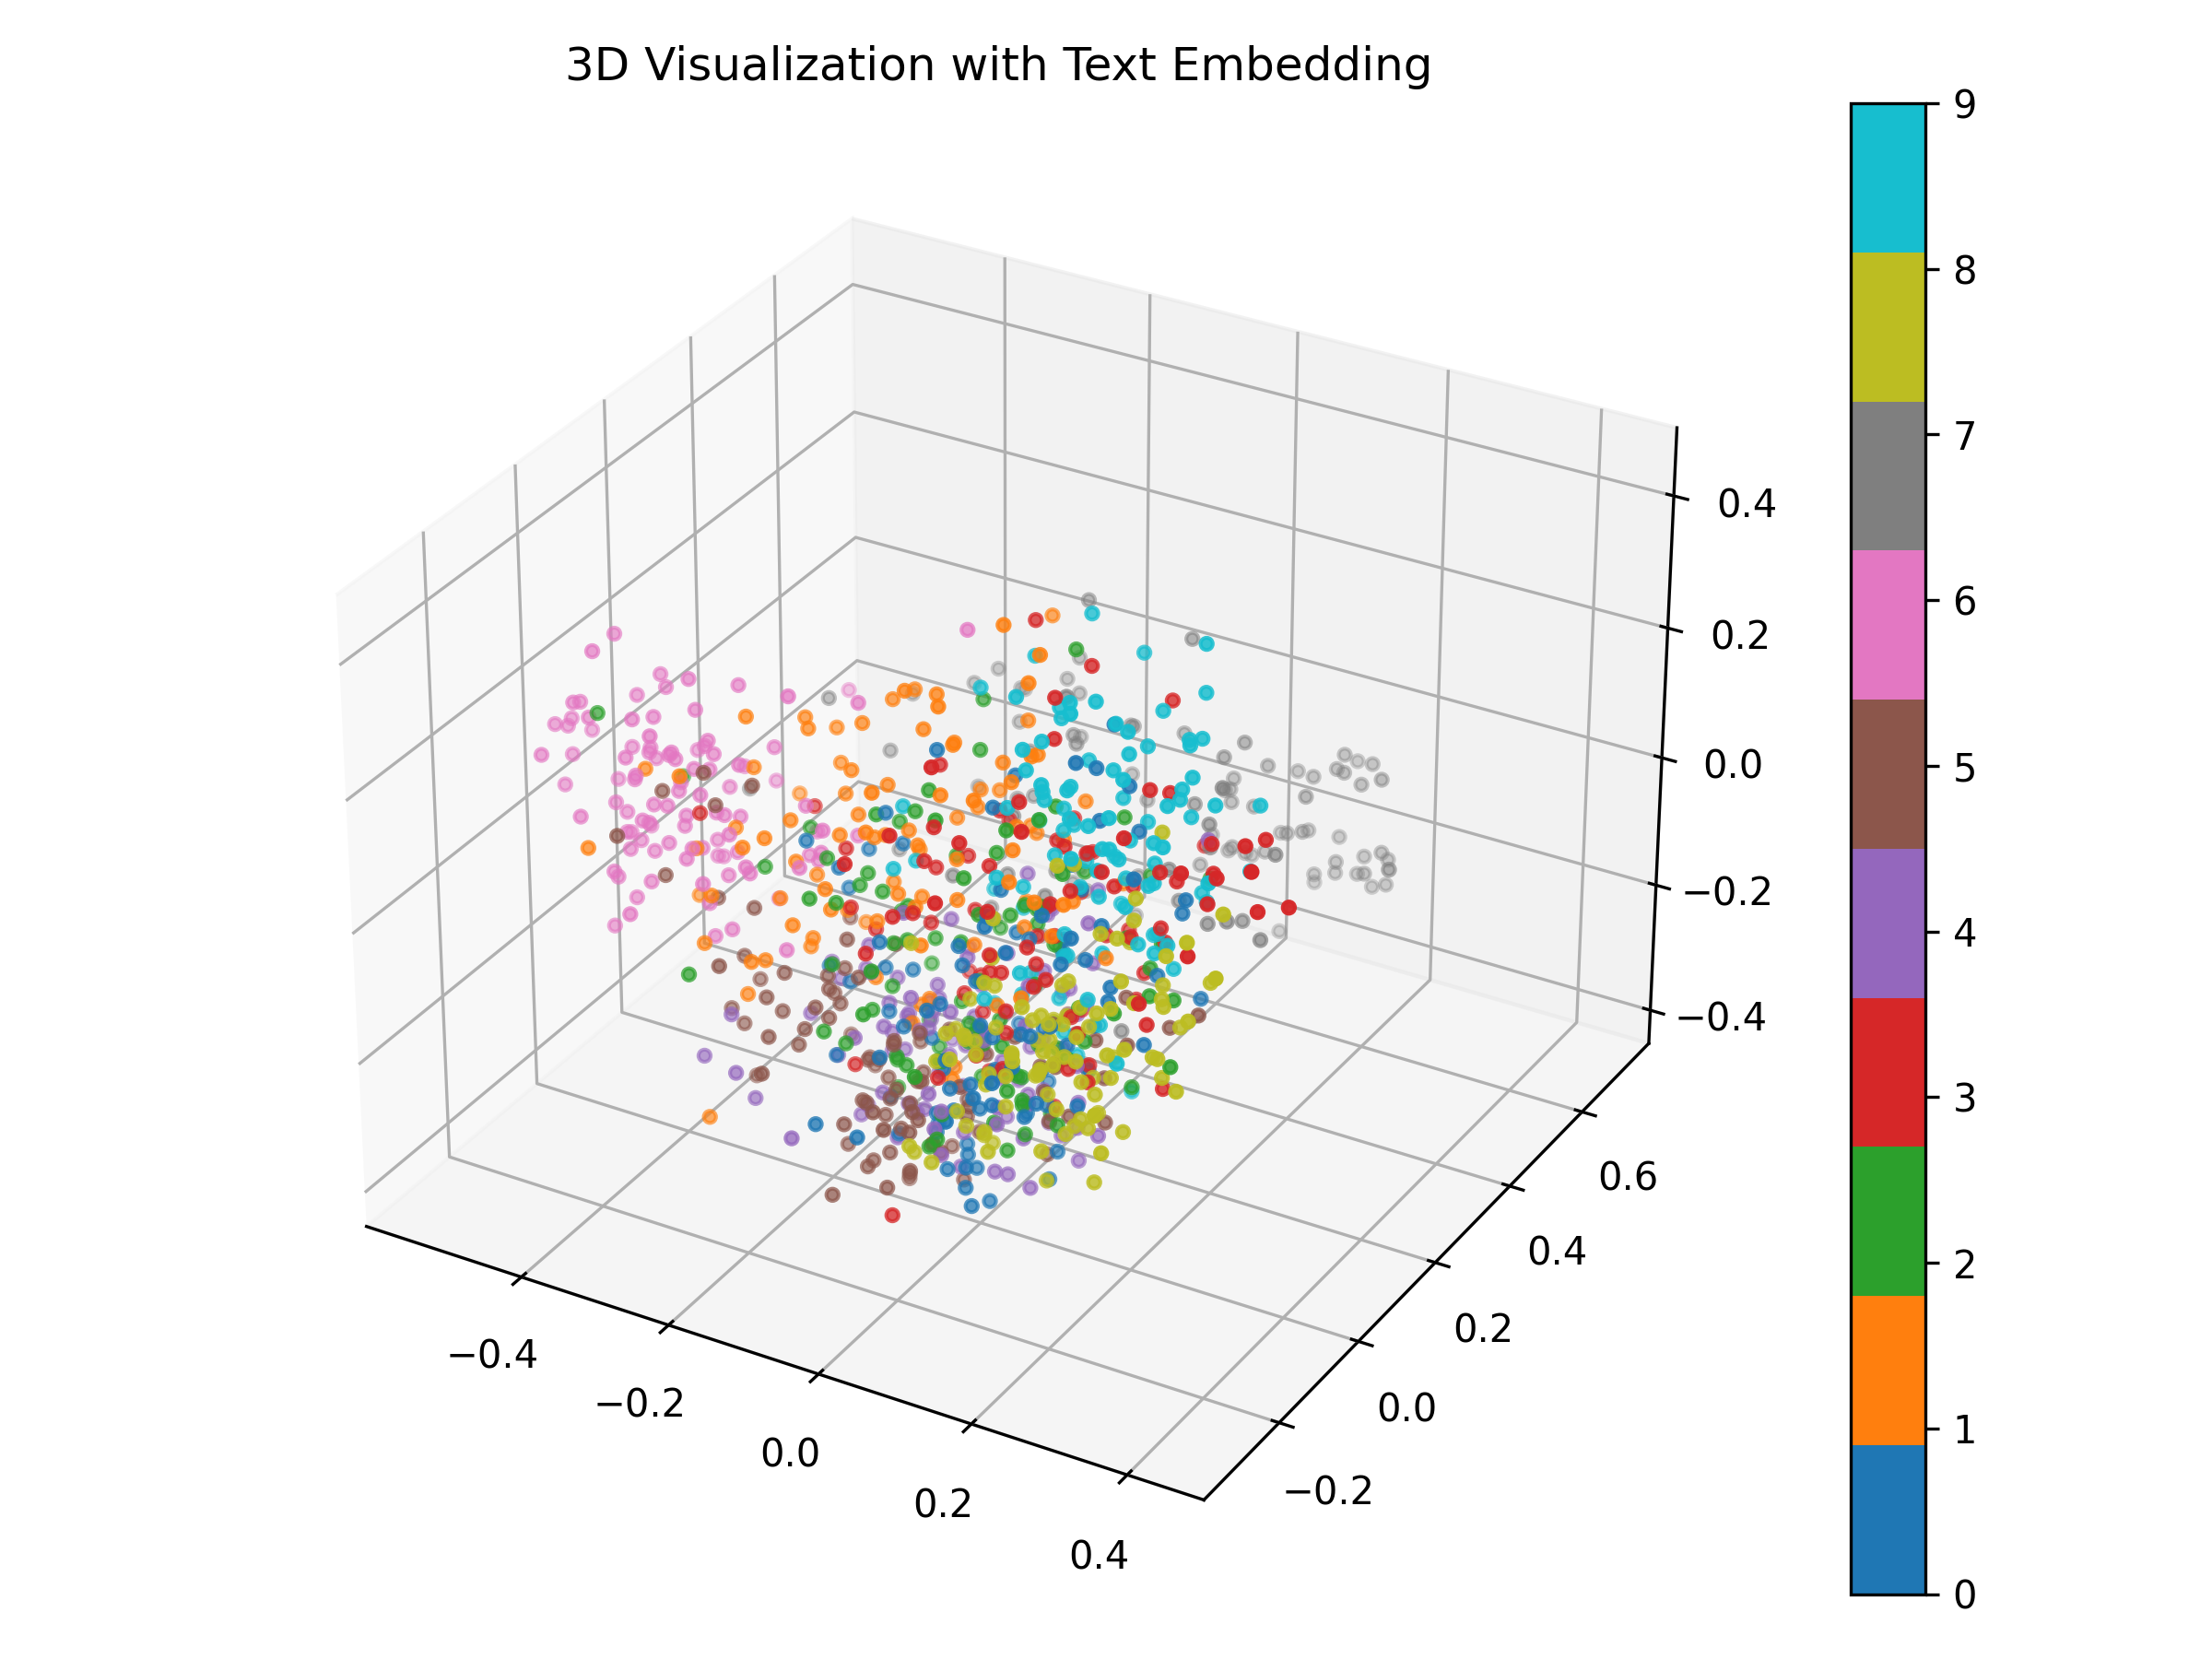
\includegraphics[width=0.3\textwidth]{
                fig/3d_visualization_embedding.png
            }
            % \subcaption{Clustering based on the sentence embedding. We visualize  100 samples in each cluster.} 
        \end{subfigure}
        \caption{(left). The number of clusters and accuracy (ACC) using Phi-3 3B. Cluster analysis. The number of clusters and accuracy (ACC) using Mistral 7B. Clustering based on the sentence embedding. We visualize  100 samples in each cluster.}
        \label{fig:cluster_performance}
    \end{figure}

    The Fig. \ref{fig:cluster_performance} shows the relationship between the
    number of clusters and accuracy (ACC) using two different model backbones: Phi-3
    3B (left) and Mistral 7B (right). For the Phi-3 3B backbone, accuracy increases
    from approximately 65.4\% at 1 cluster to a peak of 68.9\% at 10 clusters,
    stabilizing thereafter up to 15 clusters. In contrast, the Mistral 7B
    Backbone shows a more gradual improvement, rising from 63.1\% at 1 cluster
    to 64.9\% at 10 clusters. We think it is still a challenge to determine the
    ideal number of clusters. Further investigation with more sophisticated clustering
    techniques could provide deeper insights into the relationship between performance
    and the number of clusters.


\subsection{Zero-shot Results on Mistral 7B}
\label{sec:zero_shot_mistral}

For the Mistral (7B) model, the multi-task
version achieves a notable improvement, raising the accuracy from 59.5\% to
    63.1\%.
\begin{table*}[ht]
\small
\centering
\begin{adjustbox}
{width=1.0\textwidth}
\begin{tabular}{l|cccccccccc|c} 
\Xhline{1.6pt}
\multicolumn{1}{c|}{} & \multicolumn{3}{c}{\textbf{Common Sense}} & \multicolumn{4}{c}{\textbf{Question Answering}} & \multicolumn{2}{c}{\textbf{Coding}} & \multicolumn{1}{c}{\textbf{ Reasoning}} & \multicolumn{1}{c}{\textbf{AVG}} \\
\cmidrule(lr){2-4}  \cmidrule(lr){5-8} \cmidrule(lr){9-10}
\cmidrule(lr){11-11}
\multicolumn{1}{c|}{} & \textbf{Piqa} & \textbf{Wg} & \textbf{Hswag} & \textbf{Boolq} & \textbf{Obqa} & \textbf{ArcE} & \textbf{ArcC} & \textbf{HE} & \textbf{Mbpp} & \textbf{BBH} & \multicolumn{1}{c}{\textbf{AVG}} \\
\midrule

\rowcolor{lightgray}\multicolumn{12}{c}{\textbf{Mistral (7B) with LoRA library}  } \\
\textbf{BASE}  & 81.1  & 66.5  & 78.8  & 82.2 & 44.6 & 68.9 & 49.6 & 28.0 & 47.5 & 47.9 & \cellcolor[HTML]{FDE9E8}59.5\\ 
\textbf{Multi-task}  & 81.9 & 68.6 & 79.5 & 84.6 & \textbf{50.4} & 84.8 & 60.0 & 24.4 & 47.5 & 49.2 & \cellcolor[HTML]{FDE9E8}63.1 \\

\textbf{Uniform}& 82.1 & 67.2 & 79.6 & 82.7 & 45.2 & 78.7 & 54.8 & 29.9 & 49.4 & 49.0 &  \cellcolor[HTML]{FDE9E8}61.9 \\

\textbf{Ties-merging} & 82.4 & 70.6 & 79.9 & 87.6 & 44.2 & 81.1 & 57.3 & \textbf{31.7} & 47.9 & 46.2 & \cellcolor[HTML]{FDE9E8}62.9 \\
\textbf{Task Arithmetic} & 82.3 & 67.1 & 79.5 & 82.4 & 45.3 & 78.4 & 54.8 & 30.0 & 49.4 & 49.1 &  \cellcolor[HTML]{FDE9E8}61.8\\
\textbf{Ties w/DARE} & 82.3 & 70.3 & 79.8 & 87.4 & 44.3 & 81.3 & 57.2 & 31.6 & 47.6 & 46.3 & \cellcolor[HTML]{FDE9E8}62.8\\
\textbf{TA w/DARE} & 82.2 & 67.3 & 79.5 & 82.2 & 45.4 & 78.3 & 54.9 & 30.1 & 49.5 & 49.2 & \cellcolor[HTML]{FDE9E8}61.9\\
\textbf{TSV merging} & 81.6 & 70.3 & 78.9 & 82.8 & 42.8 & 84.0 & 58.3 & 28.7 & 49.7 & 49.5 & 62.7\cellcolor[HTML]{FDE9E8}\\

\midrule
\rowcolor{lightgray}\multicolumn{12}{c}{\textbf{Mistral (7B) with C-LoRA library }} \\
\textbf{Uniform}  & 82.4  & 71.4 & 81.2 & 87.6 & 49.2 & 86.0 & 60.5  & 29.3 & 50.0 & 50.0 & \cellcolor[HTML]{FDE9E8}64.9 \textcolor{red}{\scriptsize ↑2.2} \\ 
\textbf{CP-merging} & \textbf{82.6} & \textbf{71.7} & \textbf{81.6} & \textbf{87.8} & 49.3  & \textbf{86.0} & \textbf{60.6} & 29.3  & \textbf{50.2}  & \textbf{50.7} & \cellcolor[HTML]{FDE9E8}\textbf{65.0} \textcolor{red}{\scriptsize ↑2.3} \\ \hline

\Xhline{1.6pt}
\end{tabular}
\end{adjustbox}
\caption{10 downstream Zero-shot results based on Mistral 7B.}
\label{tab:zeroshot_mistral}
\end{table*}

\end{document}
